% Here is a sample format for dissertation in math.  You need to check
% University of Pennsylvania Doctoral Dissertation Manual to adjust
% any changes they made at the webpage:

% http://www.upenn.edu/grad/DissManual.html.  

% This style file was used in connection with printing from printer 3one.
% (Different printers could give you different margins.)

% This sample can also be used for masters thesis, but you need to make
% some slight changes.
    
\documentclass[12pt,letterpaper]{report}
% XXX: FORMATTING:
% http://tex.stackexchange.com/questions/132170/what-do-headheight-headsep-etc-do-in-the-vmargin-package
\setlength{\hoffset}{0.5in}
\setlength{\voffset}{0in}
\setlength{\oddsidemargin}{0in}
\setlength{\topmargin}{0in}
\setlength{\headheight}{0in}
\setlength{\headsep}{0in}
\setlength{\textheight}{9in}
\setlength{\textwidth}{6in}
\setlength{\marginparsep}{0in}
\setlength{\marginparwidth}{0in}
\setlength{\marginparpush}{0in}
%\setlength{\footskip}{30pt}
\addtolength{\textheight}{-1\footskip}
\pagestyle{plain}

% bindingoffset=0.2in,footskip=.25in
%\usepackage[letterpaper,left=1.5in,right=1in,top=1in,bottom=1in,footskip=30pt]{geometry}
%%\setlength{\topmargin}{0in}
%\setlength{\headheight}{0in}
%%\setlength{\headsep}{0in}
%\setlength{\textheight}{8.5in}
%\setlength{\oddsidemargin}{0.55in}
%%\setlength{\marginparwidth}{0in}
%%\setlength{\marginparsep}{0in}
%%\setlength{\footskip}{0.3in}
%%\setlength{\evensidemargin}{-0.25in}
%\setlength{\textwidth}{5.87in}
%\setlength{\headsep}{-.19in}

%\newcommand{\doublespaced}{\renewcommand{\baselinestretch}{2}\normalfont}
%\newcommand{\singlespaced}{\renewcommand{\baselinestretch}{1}\normalfont}
%\newcommand{\draftspaced}{\singlespaced} %for draft only 
%\newcommand{\draftspaced}{\doublespaced} %for final version
%\newcommand{\subsubsubsection}{\paragraph}


% XXX: PACKAGES:
\usepackage[comma]{natbib}
\setcitestyle{square}
\usepackage[normalem]{ulem}	                        % underlining!
\usepackage[table, usenames,dvipsnames]{xcolor}            % color
\usepackage{extarrows}                              % http://ctan.org/pkg/extarrows
\usepackage{setspace}                               % \doublespacing or \onehalfspacing
%\usepackage{showframe}
%\usepackage{enumitem}
\usepackage[tight,footnotesize]{subfigure}

% Math
\usepackage{amsmath,amssymb,amsfonts,amsthm,dsfont} % math
\usepackage{algorithm,algorithmicx,listings}        % algorithms
\usepackage[noend]{algpseudocode}			        % necessary for algorithmicx

% Figures
\usepackage{graphicx}
\usepackage{tabularx}
\usepackage{multirow,multicol,rotating,diagbox}
\usepackage{booktabs}
\usepackage{makecell}
\usepackage[font={small}]{caption}   %onehalfspacing
%\usepackage[font={small}]{subcaption}
\setlength{\belowcaptionskip}{-3.5pt}
\setlength{\abovecaptionskip}{3pt}
%\captionsetup[algorithm]{font=small}
%\usepackage[svgnames]{xcolor}
%\usepackage[breaklinks=true, colorlinks=true,linkcolor=Blue, bookmarks=true, citecolor=Mahogany, urlcolor=RoyalPurple,linktoc=all]{hyperref}
\usepackage[breaklinks=true, colorlinks=false,linkcolor=black, bookmarks=true, citecolor=black, urlcolor=black,linktoc=all]{hyperref}

\newcommand{\figref}[1]{Fig.~\ref{fig:#1}}
\newcommand{\Hao}[1]{$\clubsuit$\footnote{HAO: #1}}
% XXX: COMMANDS:
\def\liminf{\mathop{\lim\inf}\limits}	% EXAMPLE: \liminf_n A_n
\def\limsup{\mathop{\lim\sup}\limits}	%
\def\argmin{\mathop{\arg\min}\limits}	%
\def\argmax{\mathop{\arg\max}\limits}	%
% Write above and below equal sign
\newcommand{\longeq}[2]{\xlongequal[\!#2\!]{\!#1\!}}
% #1 = top; #2 = bottom; #3 = inequality (<,>,\leq,\geq)
\newcommand{\longineq}[3]{\overset{#1}{\underset{#2}{#3}}}
\newcommand{\indicator}{\mathds{1}}
\DeclareMathOperator{\tr}{tr}
\DeclareMathOperator{\per}{\mathbf{per}}
\def\deg{^{\circ}}
\def\negquad{\mkern-18mu}             % negative quad space
\def\negqquad{\mkern-36mu}            % negative qquad space
\newcommand{\txbx}[1]{\boxed{\text{#1}}}
\newcommand{\TODO}[1]{{\color{red}#1}}
\newcommand{\tcn}[1]{\cellcolor{Magenta!#1!TealBlue}#1}% table colored number
\newcommand{\tcnb}[1]{\cellcolor{Magenta!#1!TealBlue}}% table colored number
\def\negl{\scalebox{0.75}{$\boldsymbol{\ominus}$}}
\def\posl{\scalebox{0.75}{$\boldsymbol{\oplus}$}}

\makeatletter
\newcommand{\customlabel}[2]{%
   \protected@write \@auxout {}{\string \newlabel {#1}{{#2}{\thepage}{#2}{#1}{}} }%
   \hypertarget{#1}{#2}
}
\makeatother

%\newtheorem{theorem}{Theorem}
%\newtheorem{proposition}{Proposition}
%\newtheorem{corollary}{Corollary}
%\newtheorem{definition}{Definition}
\newtheorem{assumption}{Assumption}[chapter]
\newtheorem*{assumption*}{Assumption}
%\newtheorem{remark}{Remark}
\newtheorem*{problem*}{Problem}
\newtheorem{problem}{Problem}
%\newtheorem{lemma}{Lemma} 


\newtheorem{theorem}{Theorem}[chapter]
\newtheorem{corollary}[theorem]{Corollary}
%\newtheorem*{main}{Main~Theorem}
\newtheorem{lemma}[theorem]{Lemma}
\newtheorem{proposition}[theorem]{Proposition}

\theoremstyle{definition}
\newtheorem{definition}{Definition}[chapter]
\newtheorem{property}{Property}[chapter]

\theoremstyle{remark}
\newtheorem*{remark*}{Remark}
\newtheorem{example}{Example}[chapter]

\numberwithin{equation}{chapter}


% NAMED THEOREMS
% EXAMPLE:
%\begin{namedthm}{Zorn's Lemma}[Zermelo]
%All well-behaved ordered sets have maximal elements.
%\end{namedthm}
\theoremstyle{plain} % just in case the style had changed
%\swapnumbers % optional, of course
\newcommand{\thistheoremname}{}
\newtheorem{genericthm}[theorem]{\thistheoremname}
\newenvironment{namedthm}[1]
  {\renewcommand{\thistheoremname}{#1}%
   \begin{genericthm}}
  {\end{genericthm}}
  
\newtheorem*{genericthm*}{\thistheoremname}
\newenvironment{namedthm*}[1]
  {\renewcommand{\thistheoremname}{#1}%
   \begin{genericthm*}}
  {\end{genericthm*}}


\usepackage[per-mode=symbol]{siunitx}
\usepackage{paralist}

%\doublespaced
\def\thetitle{From Verified Models to Verified Code for Safe Medical Devices}
\def\theauthor{Zhihao Jiang}
\def\theyear{2016}




%====================================================================
\hypersetup{
  pdfauthor={\theauthor},%
  pdftitle={\thetitle},%
  pdfsubject={PhD dissertation},%
  pdfkeywords={cyber-physical systems,  }
  %pdfproducer={LaTeX},%
  %pdfcreator={pdfLaTeX}
}

%\addtocontents{toc}{\protect{\pdfbookmark[0]{\contentsname}{toc}}}



\begin{document}
\pagenumbering{roman}

%=================================================
%%% TITLE PAGE
\newpage
\phantomsection
\addcontentsline{toc}{chapter}{Title}
\thispagestyle{empty}
\vspace*{\fill}
\begin{center}
\thetitle

\vspace*{0.3in}
\theauthor

\vspace*{0.3in}
A DISSERTATION\\
$ $\\
in \\
$ $\\
Computer and Infomation Science\\
$ $\\
Presented to the Faculties of the University of Pennsylvania\\
in Partial Fulfillment of the Requirements for the\\
Degree of Doctor of Philosophy\\
$ $\\
\theyear
\end{center}

\vspace{0.6 in}
\noindent\makebox[0in][l]{\rule[2ex]{3in}{.3mm}}
Rahul Mangharam, Associate Professor of Electrical and Systems Engineering\\Supervisor of Dissertation

\vspace*{0.6 in}
\noindent\makebox[0in][l]{\rule[2ex]{3in}{.3mm}}
Rajeev Alur, Zisman Professor of Computer and Information Science\\Graduate Group Chairperson

\vspace*{0.2in}
\noindent Dissertation Committee:\\
Insup Lee, Cecilia Fitler Moore Professor of Computer and Information Science\\
Pieter J. Mosterman, Adjunct Professor at the School of Computer Science at McGill University\\
Richard Gray, Biomedical Engineer at FDA
\vspace*{\fill}
%=================================================




%=================================================
%%% COPYRIGHT PAGE
\newpage
\thispagestyle{empty}
\vspace*{\fill}
\begin{center}
From Verified Models to Verified Code for Safe Medical Devices

\vspace*{0.6 in}
COPYRIGHT

\vspace*{0.6 in}
\theyear

\vspace*{0.6 in}
\theauthor
\end{center}
\vspace*{\fill}
%=================================================


%=================================================
%%% DEDICATION
\newpage
\begin{center}
\vspace*{\fill}
\it{To the universe.}
\vspace*{\fill}
\end{center}
%=================================================


%=================================================
%%% ACKNOWLEDGEMENTS
\newpage
\phantomsection
\addcontentsline{toc}{chapter}{Acknowledgments}
\chapter*{Acknowledgments}
%\input{acknowledgements.tex}
Thank you, God bless you; and may God bless the United States of America
%=================================================




%=================================================
%%% ABSTRACT
\newpage
\phantomsection
\addcontentsline{toc}{chapter}{Abstract}
\begin{center}
ABSTRACT\\
$ $\\
\thetitle\\
$ $\\
Zhihao Jiang\\
Rahul Mangharam\\
\end{center}

\noindent 




 
%=================================================



%=================================================
%%% CONTENTS
\newpage
\phantomsection
%\setcounter{tocdepth}{2}
\addcontentsline{toc}{chapter}{Contents}
\tableofcontents
\clearpage
\phantomsection
\addcontentsline{toc}{chapter}{\listtablename}
\listoftables
\clearpage
\phantomsection
\addcontentsline{toc}{chapter}{\listfigurename}
%\addtocontents{toc}{\protect{\pdfbookmark[0]{\listfigurename}{lof}}}
\listoffigures
%=================================================




%=================================================
%%% MAIN
\newpage
\pagenumbering{arabic}
\setcitestyle{aysep={}} % no separation between author and year

\chapter{Medical Devices: Current State and Challenges}

The medical device market is worth \$289 billion, of which \$110 billion is from the US alone, with this number projected to reach \$133 billion in 2016.
Examples include everything from adhesive bandages, stents, artificial joints, drug infusion pumps to surgical robots, implantable cardiac pacemakers, and devices still undergoing basic research like the artificial pancreas.
To take one example of the societal impact of medical devices, an estimated 3 million people worldwide have implanted cardiac pacemakers (a heart rate adjustment device), with 600,000 added annually.
Clinical trials have presented evidence that patients implanted with cardiac defibrillators (another heart rate adjustment device) have a mortality rate reduced by up to 31\%.
% MADIT II trial
Implanted cardiac pacemakers and defibrillators have approximately 80,000-100,000 lines of software code which essentially makes all sensing, control and actuation decisions autonomously within the human body, over the 5-7 year device lifetime \footnote{Paul L. Jones. Senior Systems/Software Engineer, Office of Science and Engineering
Laboratories, U. S. FDA. Personal communication, 2010.}. With the increasing complexity of combining hardware and software in a large class of these life-saving technologies, there is an urgent need for approaches to rigorously validate the device and therapy to be safe and efficacious.
\begin{figure}[t]
		\centering
		\includegraphics[width=\textwidth]{figs/devices_new.pdf}
		\caption{\small Current medical devices across a range of diagnostic and therapeutic risk. Implantable software-controlled devices such as the pacemaker and defibrillator which operate in a closed-loop of sensing, control and actuation are amongst the highest risk}
		\label{fig:Cur}
\end{figure}

The US Food and Drug Administration defines a medical device as an instrument, apparatus, implement, machine, or implant which is:
\begin{itemize}
	\item intended for use in the diagnosis of disease or other conditions, or in the cure, mitigation, treatment, or prevention of disease, in humans or other animals, or
	\item intended to affect the structure or any function of the human body or other animals, and which does not achieve any of its primary intended purposes through chemical action and which is not dependent upon being metabolized for the achievement of any of its primary intended purposes."
\end{itemize}
\newpage
In general, medical devices are categorized according to their risk factors - Class I, Class II and Class III, corresponding to low-risk, medium-risk and high-risk devices (\cite{class}).  \figref{Cur} gives an intuitive description of medical devices examples across a range of diagnostic and therapeutic risk.


%%On similar lines, in the European Union there are five medical devices categories based on non-invasive vs. invasive, length of stay in body, contact with blood vessels or the central nervous system, active vs. non-active and implantable devices. (\cite{EU_classify}) 
%%Invasive devices with active interventions are subject to stringent regulations to ensure the patient's safety and efficacy of therapy.
\begin{figure}[t]
		\centering
		\includegraphics[width=\textwidth]{figs/closed-loop.pdf}
		\caption{\small Diagnostic-only and therapy-only devices do not interact with the patient in direct closed-loop. The physician is responsible for the diagnostic and/or therapeutic decisions. However in closed-loop medical devices, the devices interact with the patient in closed-loop and have to make therapeutic decisions based on their own diagnosis.}
		\label{fig:closed-loop}
\end{figure}
\section{Closing the Device-Patient Loop}
Medical devices operate across a range of invasiveness and intervention with the patient in the loop. For diagnostic-only devices, like an X-ray machine, the physician operates the device to obtain patient data. Upon interpretation of the data, the physician performs diagnosis followed by delivery of proper therapy to the patient (\figref{closed-loop}.(a)). For therapy-only devices, e.g. a drug infusion pump, the physician configures the device infrequently based on prior diagnosis of the patient so the device executes the therapy on the patient (\figref{closed-loop}.(b)). We denote these devices as \textbf{Open-loop Medical Devices} as there is no direct feedback loop between the patient and the device. For open-loop devices, the device operates under the supervision of professionally-trained physicians. The device's safety is mostly determined by how accurately it provides information to the physicians or how faithfully it operates as instructed by the physicians.

There is a class of devices with both diagnostic and therapeutic functions, i.e. implantable cardiac devices to treat cardiac arrhythmia, deep brain stimulation devices (\cite{Brain_sti}) to treat Parkinson's disease and artificial pancreas to treat Type-1 diabetes. These devices capture and diagnose the patient's physiological conditions from sensory data, \emph{and} deliver therapy in response (\figref{closed-loop}.(c)). These devices usually operate (semi-) autonomously with very little human intervention. 
The benefits of closed-loop medical devices are timely therapy and better life-style.
However, autonomy of these medical devices also arose safety concerns. 
Malfunctions or inappropriate therapies from these devices also cannot be corrected timely, which can cause serious adverse effects on patients' health. 
With open-loop medical devices, the diagnosis and therapy decisions are made by medical professionals, who have expert knowledge of human physiology. Therefore they are able to identify adverse health conditions and adjust the therapy accordingly. On the other hand, closed-loop medical devices have to make both the diagnosis and therapy decisions on their own. The domain expertise required to make those decisions has to be programmed into the device. It is impossible to encode all the knowledge of human physiology into the device. Therefore, for unanticipated physiological conditions, when the appropriate response has not been programmed into the device, the device may deliver inappropriate therapy which can have an adverse effect on patient's health. 
Therefore, these devices are usually classified into the highest risk category and undergo the most stringent regulation. We denote them as \textbf{Closed-loop Medical Devices}. 

There are multiple challenges to develop safe and effective closed-loop medical devices:

\subsection{Physiological Complexity:} Human physiology is complex and only partially understood. For instance, the functionality of the heart can be interpreted from \emph{multiple perspectives}: from its electrical activity, mechanical contractions of the heart muscles, and dynamics of blood flow. The physiology of the heart can also be analyzed with \emph{multiple scales}: from the molecular level to cellular level all the way to the organ and system level. It is impossible to encode all these contexts into the device, hence inappropriate diagnosis and therapy are observed due to the lack of physiological contexts~\cite{killedbycode, icd_recall}.
	\subsection{Physiological Variability:} Physiological conditions and parameters demonstrate different levels of variability both within the individual at different times, levels of exertion and under the influence of medication and also across individuals. For instance, a segment of the population may have additional conduction pathways within their heart, which makes them vulnerable to certain heart diseases. Consequently, autonomous medical devices should be able to safely operate under a large variety of physiological conditions. This is difficult to guarantee, as the device designer must consider all possible physiological conditions (including rare conditions) during the design of the device.
	%\hatodoin{last sentence: rather than say "always", say something like: "the designer will likely miss some rare conditions during the design of the device".}
	
	\subsection{Limited Observability:} Autonomous medical devices normally rely on minimally invasive measurement of the physiological parameters in order to allow the patients to live their normal life. For example, implantable pacemakers and defibrillators commonly have just two leads and therefore two points of observation for the whole heart. The limited observability inevitably leads to ambiguities as different physiological conditions can map to the same input sequence to the device, resulting in inaccurate diagnosis. 

\subsection{Software-related Medical Device Recalls}
Due to the complexity of the diagnostic and therapeutic functions of the closed-loop devices, these functions are mostly controlled by their software components. 
Software embedded in a medical device, unlike electrical and mechanical components, does not fail due to corrosion, fatigue or have statistical failures of subcomponents. Software failures are uniquely sourced in the design and development of the system. %Unlike other industries such as consumer electronics where product life cycles are measured in months, software engineering for medical devices often spans a decade and must prioritize safety and efficacy over time to market. 
%\begin{figure}[t]
		%\centering
		%\includegraphics[width=0.8\textwidth]{figs/recalls.jpg}
		%\caption{\small Medical device recalls have risen over the past decade}
		%\label{fig:recalls}
%\end{figure}
\begin{figure}[t]
		\centering
		\includegraphics[width=0.8\textwidth]{figs/recalls.pdf}
		\caption{\small Medical device recalls due to software issues have risen from 10\% in the 1990s to \~15\% in the past decade (\cite{recall_rep})}
		\label{fig:soft_recalls}
\end{figure}
%  Over the course of the past four decades, cardiac rhythm management devices such as pacemakers and implantable cardioverter defibrillators (ICD) have grown in complexity and now have more than 80,000 to 100,000 lines of code (\cite{pauljones}). 
According to the US Food and Drug Administration, in 1996, 10\% of all medical device recalls were caused by software-related issues (\cite{medstats}). This percentage rose to an average of 15\% of recalls from 2008 to 2012 (\figref{soft_recalls}). Malfunctions of closed-loop medical devices usually have severe consequences, which will be categorized as \emph{Class I}, meaning there is a ``reasonable probability that use of these products will cause serious adverse health consequences or death.'' (\cite{medstats2,pacemakerrecalls,killedbycode}). 
\looseness1
\section{Medical Device Regulation Efforts and Challenges}
The medical device industry is regulated to ensure the safety of the patients and the public. In the United States, the FDA is the primary regulatory authority responsible for assuring the safety, efficacy and security of patients using medical devices. 

%\begin{itemize}
	%\item Efficacy: The device is effective in achieving its intended and expected use.
	%\item Safety: The device does not expose the patient, user, or other bystanders to undue risk from its use;
	%\item Security: The device has been designed to protect patients, users, and bystanders from both unintentional and malicious misuse of the device
%\end{itemize}

Based on the rationale that 1) manufacturers know their devices better than the regulator, and 2) the variety of medical devices requires a variety of approaches, it is the device manufacturers' responsibility to demonstrate the safety and efficacy of the medical devices. Manufacturers are required to complete a pre-market submission before the devices can be released to the market. The level of requirements for the submission is determined by the safety classification of the devices. A set of general guidelines are recommended by the FDA (\cite{fda1, fda2, fda3}) which list the activities that need to be performed to ensure device safety. 

In safety-critical industries such as automotive electronics, avionics and nuclear systems, international standards are \textbf{enforced} for software system development, evaluation, manufacturing and post-market changes (\cite{autosar,avsi}). This awareness is only beginning to enter the medical device industry as compliance with international standards are "recommended" in the aforementioned guidelines (\cite{formal_fda}) but the burden of their interpretation and enforcement is on the device manufacturer. The basic rationale behind these standards is that: if all the risks/hazards of the device are identified and reasonably mitigated, and the device is developed with rigorous process, the device is \emph{reasonably safe}. 
\begin{figure}[t]
		\centering
		\includegraphics[width=0.6\textwidth]{figs/stardards.pdf}
		\caption{\small International standards for medical device safety. These standards define the required activities during the development process.}
		\label{fig:standards}
\end{figure}

\figref{standards} describes the primary standards to ensure medical device safety and their relationships. The IEC 60601 Medical Electrical Equipment - General requirements for basic safety and essential performance is a product safety standard that all electronic medical devices must comply to. IEC 60324 specifies the processes and activities needed to perform during the software development life cycle to ensure software safety. 

Risk management is a core activity throughout the software development life cycle. ISO 14971 is specified for the application of risk management to medical devices. In addition, for each risk management activity of ISO 14971, ISO 80002-1 provides additional guidelines for the software component, which highlights and explains approaches to assuring that software safety is adequately addressed.

%While the above standards and several others provide guidelines to ensuring software safety they do so in an informal or ad hoc manner with a focus on the rigorousness of the design process rather than on quantitative evaluation on the closed-loop system with the physiological system (or a model) and the feedback to and from the device. Furthermore, there is a separation of concerns where the \emph{regulatory perspective} is on the overall safety of the device meeting its diagnostic and therapeutic requirements within its environment (e.g. pacemaker inside the body and connected with the heart tissue), the \emph{software standards' perspective} is on the device meeting its specifications (e.g. if the pacemaker does not sense an event within a certain interval, then pace the heart). While the device may respond appropriately to the sensed input, we also need to establish that the device never drives the patient to an adverse condition. As the regulatory perspective requires closed-loop safety and the device software's specifications are largely evaluated with open-loop ``tape tests" of pre-recorded signals, with no physiological interaction, this introduces a safety gap.  So a device may meet its software specifications but that does not necessarily ensure it meets the physiological safety requirements. 


%The history of the FDA is a reactionary one, where each stage of evolution was in response to a major healthcare tragedy. 
%\begin{figure}[t]
		%\centering
		%\includegraphics[width=\textwidth]{figs/fta_new.pdf}
		%\caption{\small Fault Tree Analysis (FTA) Examples. (a) FTA for a hazard for a car; (b) FTA for a hazard in implantable pacemaker. The dashed line shows two mechanisms that were not identified during hazard analysis but discovered in post-market studies.}
		%\label{fig:risks}
%\end{figure}
%\subsection{Risk Management Challenges of Closed-loop Systems}
%While it is not normally possible to develop a device that is safe with a probability of 100\% under all physiological and operating conditions, approaching the problem along the lines of risk analysis, risk evaluation and risk control helps better address a ``designed-for-safety" mindset. Fault Tree Analysis (FTA) is a common tool in risk analysis in which hazards of the system are first identified and the possible causes of the hazards are analyzed until the initial faults are reached. \figref{risks}.(a) demonstrate an example fault tree for automobile. FTA is very good at showing how resistant a system is to single or multiple initiating faults. It is not good at finding all possible initiating faults since causes are conjectured and analyzed manually. 
%
%In closed-loop medical devices, there may exist interactions between the device and the patient that can cause certain hazard, but are unknown due to limits in physiological knowledge, behavior not captured in patient trials and the separation of the software development teams and the medical domain experts. \figref{risks}.(b) describes an example fault tree for a hazard for an implantable pacemaker. There are several causes for undesirable fast ventricular rate. The well-understood cause is the intrinsic ventricular tachycardia (solid line). However, with pacemaker implanted, new mechanisms to cause hazard are introduced into the closed-loop system, as illustrated by the two branches with dotted lines. These two branches were not identified during the initial fault tree analysis, and were only identified after the devices have been released into the market, causing unnecessary adverse effects to the patients \cite{ELT}. Risks identified at this late stage are also more costly to fix, increasing the cost for device development. 
%
%
%\begin{figure}[t]
		%\centering
		%\includegraphics[width=\textwidth]{figs/risk_analysis.pdf}
		%\caption{Top table: Risk index according to occurrence and severity. Bottom table: Risk control using risk index}
		%\label{fig:risk_ana}
%\end{figure}
%
%After the fault tree has been constructed, probabilities for the initial faults are analyzed bottom up to calculate the probability of each hazard. The technique is called Failure Mode and Effects Analysis (FMEA). Then the risks are evaluated by assigning risk index to each hazard according to their occurrence and severity (\figref{risk_ana}). After the risks are evaluated, different activities are required to mitigate the risks according to the risk index. The risks are then be re-evaluated to calculate the residual risk and analyze the risk/benefit. This is part of the risk control process. FMEA is good at exhaustively cataloging initiating faults, and identifying their local effects. It is not good at examining multiple failures or their effects at a system level.

\subsection{Pre-Market Evaluation with Clinical Trials}
Regardless of how rigorous the risk management and the device development process are, the devices have to be able to achieve their design goal on the real patient, which can only be evaluated within its physiological environment. Devices that have high risk factors, including the closed-loop medical devices, are required to submit clinical evidence for their safety and efficacy, often in form of clinical trials. In clinical trials, the devices are used on a preselected population of patients following carefully-designed protocols. The goal of a medical trial, in part, is  to obtain unambiguous results for the primary question of the trial which can support the safety and/or efficacy of the devices. However, conducting clinical trials is very time consuming and expensive, and risks found during clinical trials are very expensive to fix (\cite{trialcost}). 

To address this \textbf{safety gap} between ensuring the device satisfies its therapeutic requirements with the patient-in-the-loop and testing its software specifications, new approaches for closed-loop validation of the device software within the physiological context are needed - this is the primary focus of this article.
%Through the course of the 1980s, software began to play an increasing role in medical devices. Software, as it turns out, is one of those technologies not anticipated by prior regulation, and was waiting for its disaster to prompt regulatory action. It wasn't until the 1980s when a number of cancer patients received massive X-ray overdoses during radiation therapy with the Therac-25 linear accelerator. This lead to a number of investigations, perhaps the most thorough of which was that of \cite{therac}, which was rich with identified ways software could go wrong. Inadequate testing, dangerous code reuse, configuration management issues, inadequate manufacturer response, and failure to get to the root cause of the problem were among the leaders of the problems identified. The Therac-25 was an eye-opener for the FDA and legislators, and resulted in the Safe Medical Device Act of 1990. This finally required closer medical device tracking, post-market surveillance and recommendations on development, testing and validation of medical device software. \todo{Are these useful?}

%\subsection{Pre-market Submission Process}

%There are two processes through which a medical device can enter the market in U.S.: the Premarket Notification, also known as 510(k) \cite{510k}, and the Pre-Market Approval (PMA) \cite{PMA}. In a 510(k) submission the device manufacturers are only required to provide evidence that the device is \emph{substantial equivalent} to a \emph{predicate device}, which has been approved for the market. Therefore, the 510(k) submission does not directly require clinical evidence for the safety and effectiveness of the device, thus it is suitable for mostly low-risk devices like Class I and Class II devices.  The Pre-Market Approval (PMA) submission is a more stringent regulatory process in which direct clinical evidence is required to prove the safety and effectiveness of the device. However, not all Class III devices are subject to PMA submission. If a Class III device clears the 510(k) process and FDA has not requested PMA for that device, the device is still cleared for market release. A study shows that for Class III devices which PMA has been requested, the levels of evidence varies. Only 40\% of the PMA submissions are supported by controlled clinical trials, which provide the most rigorous clinical evidence \cite{cert_prob}. The lack of quality evidence is usually due to the high cost of the controlled clinical trials.

%\subsection{Safety and Efficacy Evidence}

%\todo[inline]{List of software standards}

%The FDA currently does not request or review the medical device software during pre-market submission. This is currently satisfied by the documentation of code inspections, static analysis, module-level testing and integration testing and their purpose is to establish ``reasonable assurance of safety and effectiveness''. These tests however fail to check for the correctness of the software and are largely open-loop tests that do not consider the context of the patient. Software is reviewed by the FDA only in the incident of a device recall. Software-related recalls are often issued in the form of \emph{Safety Alerts} by the %%%%%Food and Drug Administration (FDA) 
%FDA such as ``Safety alert - Pacemaker may revert to VVI mode at 70 beats/min if programmed to one of several specific ventricular pulse widths" (\cite{medstats}).


%\section{Challenges to Develop Safe Medical Device Software}
%\subsection{Safe Development Process vs. Safe Product}
%Conformance to the safety standards provides strong confidence on a safe development process. The belief is that a well-planned, systematic engineering process produces more reliable devices, especially if software is a component of the device (\cite{med-book}). However, there is no guarantee that safe process always yield safe devices. Recently there is growing interest on enforcing safety and efficacy evidence for the device itself. \cite{Wassyng} Due to the large variety of medical devices, there does not exist general safety and efficacy requirements that can be written into standard. As the result, evidence for product safety and efficacy varies in quality and organization. Assurance cases \cite{} have been proposed to help constructing safety arguments and organizing safety evidences. Assurance cases are currently "Recommanded" by FDA during regulation submission. (\cite{})


%\subsection{Multiple Stakeholders}
%For each medical device, there are 4 stakeholders: the regulator, the device manufacturer, the medical professional and the patient. All parties have the incentive to ensure the safety and efficacy of the device. With current regulation framework, the evidence for safety 
%\begin{figure}[t]
		%\centering
		%\includegraphics[width=0.8\textwidth]{figs/stakeholders.pdf}
		%\caption{\small Figure of current medical devices}
		%\label{fig:Cur}
%\end{figure}
%However, the medical domain presents its own unique set of challenges:\\
%\textbf{1. Closed-loop context:} Current evaluation of devices is open-loop and is unable to ensure the device never drives the patient into an unsafe state. Medical device testing and validation must thus be within the closed-loop context of the patient physiology. The context of the patient is a function of both the environment and the input from the device controller and must be captured by the device evaluation process.\\ 
%\textbf{2. Patient models:} There is a scarcity of patient models and clinically-relevant simulators for device design (\cite{pat-model}). High-fidelity models of interaction between the patient and device are needed to evaluate the safety and efficacy of device operation. Furthermore, these models must integrate the functional and formal aspects so that testing and verification are evaluated for the same patient states.\\
%\textbf{3. Adaptive patient-specific algorithms:} The therapy offered by the device must adapt to the environment and specific patient's condition. There is a need for validation algorithms to ensure that device control and optimization can cover large classes of patient conditions. 

%\section{The FDA and Medical Device Software}
%Before we delve into the current state of medical device software, it is useful to understand the evolution of the regulatory environment. 




%\section{Current Testing, Validation and Verification Approaches}
%In order to facilitate the early detection and correction of any software defects, the FDA has focused on infusion pumps due to the large number of recalls. In April 2010, the FDA began the ``Infusion Pump Improvement Initiative" which offers manufacturers ``the option of submitting the software code used in their infusion pumps for analysis by agency experts prior to premarket review of new or modified devices." 	\cite{}
%
%An effective software verification methodology is therefore needed for the risk analysis and certification of medical device software during the pre-market submission phase. While formal methods of verification are used for medical device software (\cite{challenge, challenge2, challenge3}), testing continues to be required because it can expose different kinds of problems (e.g. compiler bugs), can examine the program in its system context, and increases the diversity of evidence available. Testing for medical device software currently is ad hoc, error prone, and very expensive. Traditional methods of testing do not suffice as the test generation cannot be done independently of the current state of the patient and organ. The primary approach for system-level testing of medical devices is unit testing using a playback of pre-recorded electrogram and electrocardiogram signals (\cite{testing_imd, Vip}). This tests if the input signal triggers a particular response by the pacemaker, but has no means to evaluate if the response was appropriate for the patient condition. Furthermore, this approach of ``tape testing''\Hao{elaborate} is unable to check for safety violations due to inappropriate stimulus by the pacemaker. Pacemaker Mediated Tachycardia (PMT), a condition that is described later in this paper, is a strong example of why we need a model of the heart such as the one presented in this paper, which can be used for closed-loop system analysis. 
%PMT is a condition where the pacemaker inappropriately drives the heart-rate toward the upper rate limit. With a tape test, PMT would not occur and the response of the pacemaker could be classified as appropriate therapy.
%\begin{figure}[t]
		%\centering
		%\includegraphics[width=0.8\textwidth]{figs/heartmodel.pdf}
		%%\vspace{-5pt}
		%\caption{\small By extracting timing and electric conduction information we model the signal activation, refractoriness and propagation across the heart tissue as a set of node and path automata.}
		  %%\vspace{-15pt}
		%\label{fig:heartmodel}
%\end{figure}
%As the testing environment (i.e., patient condition) is not entirely under the control of the tester, the problem changes significantly as a degree of nondeterminism is introduced in the process. Implantable medical devices are a primary example of Medical Cyber-Physical Systems where the safety and efficacy of the device and device software must be evaluated within a closed-loop context of the patient. The key challenge is in the generation of physiologically relevant tests such that the device does not provide inappropriate therapy, and does not adversely affect the safety of the patient. In addition, test generation must be interactive and adaptive such that the previous test stimulus affects the current state of the patient. The test generator must consider the current state when generating the next input in a way that advances the purpose of the test. The problem becomes one of the controller synthesis problems and cannot be addressed by an off-the-shelf model checker~\cite{rushby}.  
   %
%Formal methods have traditionally been used for verification of time-critical and safety-critical embedded systems \cite{form-meth}. Until recently, these methods have not been used for medical device certification. \cite{med-form3} presented the use of Extended Finite State Machines for model checking of a resuscitation device. Formal techniques have also been applied to improve medical device protocols (\cite{med-form2}) and safety (\cite{med-form1}), but the authors either used a simplified patient model or did not model the patient at all. 
\section{Model-based design to improve medical device safety}
With the deluge of software-based closed-loop medical devices in the coming years, relying on clinical trials as the only closed-loop evaluation method to identify risks rooted in device software is not scalable. Model-based design and virtual integration have been proposed and applied in other industries like automotive and avionics (\cite{autosar, avsi}), and can potentially help during the development process and provide extra confidence to the device before conducting clinical trials. However, unlike man-made systems like automobiles and aircrafts, physiological systems are less understood with larger variations for the type and degree of patient conditions. The lack of faithful models of physiological environment of the closed-loop medical devices is one of the reason that model-based design is not well-adopted in the medical device industry. 
\begin{figure}[t]
		\centering
		\includegraphics[width=\textwidth]{figs/MDIC.pdf}
		\caption{\small Percentage of computer simulation is expected to increase as safety and effectiveness evidence of medical devices}
		\label{fig:MDIC}
\end{figure}

As computational models of human physiology are developed, they can be used to interact with closed-loop medical devices or their models. The FDA is starting to recognize in-silico modeling and simulation as regulatory-grade evidence for device safety and efficacy. For example, \cite{pancreas_paul} developed glucose-insulin models that can be used to evaluate control algorithms for artificial pancreas devices which can sense blood glucose and deliver insulin. Simulation results with the models have been recognized by FDA to replace animal trials, in part, which significantly reduced cost (\cite{pancreas}). With the increasing interest and recognition from the regulators, computer models and simulations are expected to play bigger role as as ``regulatory-grade evidence" evidence in the development of future closed-loop medical devices (\figref{MDIC}).

\section{Contributions}
In this thesis, I use implantable cardiac devices as working examples to demonstrate how model-based approaches can help improve the safety and efficacy of autonomous medical device. We demonstrate the application of model-based approaches in several design and pre-regulation activities, from the perspective of the manufacturer's design validation team. We assume availability of design artifacts including pacemaker design and physiological requirements. By demonstrating the process of developing verified models to generate verified code, the results of our model-based closed-loop validation should be able to support the device's safety and efficacy requirements during the regulation process.
\begin{figure}[t]
		\centering
		\includegraphics[width=0.9\textwidth]{figs/model_based_b.pdf}
		%\vspace{-5pt}
		\caption{\small Model-driven design for verified models to verified code for the closed-loop heart and pacemaker system}
		  %\vspace{-15pt}
		\label{fig:modeling_overview}
\end{figure}

In this thesis, I propose a model-based design framework for closed-loop validation of medical devices, and use implantable cardiac devices as case study.
Fig. \ref{fig:modeling_overview} demonstrates our model-based design framework for implantable pacemaker software.
The thesis can be broken down into 4 themes, which are illustrated in \figref{modeling_overview}. 

The remaining thesis is arranged as follow:
Chapter 2 discusses a dual chamber pacemaker desig n(\cite{compass}) as the motivating example to illustrate the safety hazards that the device may pose to the patients.
Chapter 3 discusses the physiological models that are necessary for closed-loop evaluation of medical devices, and how to use those models to represent complex physiology with large variability \cite{VHM_proc}.
Chapter 4 discusses the use of model-checking techniques to evaluate the safety and efficacy of device design early in the device design stage, with focus on the abstraction and refinement of the heart models to cover large variety of physiological conditions (\cite{STTT13}).
Chapter 5 discusses the rigorous translation from verified device model to device implementation which maintains the verified properties (\cite{RTAS12})..
Chapter 6 discusses the use of physiological models to generate a virtual patient population and the device can go through model-based clinical trials which can provide useful insights for planning a clinical trial on real patient.

%The contribution of this effort is three-fold: (a) We developed an integrated functional (i.e., clinically-relevant) and formal (i.e., timed automata based) Virtual Heart Model  (VHM) (see \figref{heartmodel}) and a pacemaker device model for interactive and clinically relevant test generation.  (b) We provide a set of general and patient condition-specific pacemaker software requirements to ensure the safety of the patient is met under all cases, and (c) We provide a means to test and verify the closed-loop system over a variety of basic operation tests where the heart rate must be maintained, the atrial-ventricle synchrony must be enforced and complex closed-loop tests, where the pacemaker must not initiate tachycardia or perform improperly during lead displacement. With this approach of model-based testing, an executable functional model of the pacemaker is created at an early stage in the development process. This model-based methodology is an early step in addressing the urgent need for pre-market evaluation of medical device design and certification.

\section{Useful terminologies for often misinterpreted terms}
Ensuring the safety of complex medical devices has drawn interest not only from stakeholders like regulators and industries, but also medical professionals and academia. Different communities have different interpretations over certain terminologies, often causing misunderstandings. In this paper we adopt the terminologies from the regulation perspective, so that the results we have fit into the regulation framework. Most of the definitions are referred from the FDA guideline document General Principles of Software Validation (\cite{fda2}). Below are several terminologies that we use throughout the paper which worth clarifying.
\subsection{Requirements vs. Specifications}
By the definition of FDA (\cite{fda3}), the requirements of a system describe \textbf{what} the system should achieve and the specifications of a system describe \textbf{how} the system is designed to satisfy the requirements. For example, a requirement for an autonomous car is "The car should not hit objects". The corresponding specification can be "brake if the speed of the car is greater than $x$ and the distance to the object is less than $y$". We can see that a car satisfying its specification may not satisfy the requirement (e.g. when the car is driving too fast or the obstacle pops up right in front of the car). In this paper, we use the word requirement in particular to denote the intended uses of the medical devices to improve physiological conditions.

\subsection{Validation vs. Verification vs. Testing}
As defined in \cite{fda2}, software validation is the confirmation by examination and provision of objective evidence that:
\begin{enumerate}
	\item software specifications conform to user needs and intended uses, and 
	\item the particular requirements implemented through software can be consistently fulfilled
\end{enumerate}
The first aspect ensures the device is safe and effective. The second aspect maintains the traceability of requirements throughout the development life cycle.
Software verification fulfills the second aspect of software validation by "providing objective evidence that the design outputs of a particular phase of the software development life cycle meet all of the specified requirements for that phase. "
\begin{figure}[t]
		\centering
		\includegraphics[width=\textwidth]{figs/validation.pdf}
		\caption{Validation activities during the software development life cycle (\cite{Vogel})}
		\label{fig:validation}
\end{figure}

Testing is the technique that can be used for validation and/or verification. \figref{validation} illustrates the relationship between validation, verification and testing, and different activities during the software development life cycle to ensure the safety and effectiveness of the software.
\subsection{Closed-loop vs. Open-loop Evaluation}
In open-loop evaluation, i.e. open-loop testing, input sequences are send to the system and system outputs are compared with expected outputs. In open-loop testing, the system outputs do not affect the inputs afterward. In closed-loop evaluation, the environment of the system is taken into account. System outputs affect the state of the environment and thus affect the input sequences. For closed-loop medical devices, clinical trials are currently the most common closed-loop evaluation method. Enable closed-loop evaluation at model level requires models of the environment, which is human physiology for closed-loop medical devices.

Closed-loop evaluation accomplishes two goals in model-based design: 1) It enforces environmental constraints so that the test space is smaller and the test cases have physiological relevance. 2) Execution traces can be better interpreted as the physiological models encode domain knowledge. 
%%Through each of the chapters to follow, we cover different aspects of modeling the physiological system and the device, validating the models, running model checking on the closed-loop system and testing the deterministic systems derived from the abstract models. With the goal of 

%%The US Food and Drug Administration defines medical device an instrument, apparatus, implement, machine, contrivance, implant, in vitro reagent, or other similar or related article, including a component part, or accessory which is:
%%\begin{itemize}
%%	\item recognized in the official National Formulary, or the United States Pharmacopoeia, or any supplement to them
%%	\item intended for use in the diagnosis of disease or other conditions, or in the cure, mitigation, treatment, or prevention of disease, in man or other animals, or
%%	\item intended to affect the structure or any function of the body of man or other animals, and which does not achieve any of its primary intended purposes through chemical action within or on the body of man or other animals and which is not dependent upon being metabolized for the achievement of any of its primary intended purposes."
%%\end{itemize}
\chapter{A Motivating Example: A Dual Chamber Pacemaker Design}
In this chapter we introduce a dual chamber pacemaker specification.
It is used throughout the thesis to demonstrate how different model-based techniques can be used to validate the safety and efficacy of the pacemaker.
\section{Physiology Basis of the Heart and the Pacemaker}
First, we use this small section to introduce the physiology basis of the heart and the application of implantable cardiac devices. Readers with knowledge of this subject can skip to the following sections.
\subsection{Blood Circulation System}
The heart is the "motor" for blood circulation within our body. The heart has two ventricles which pump the blood out of the heart, and two atria which gather blood from the body and pump them into the ventricles. (\figref{circulation}.(a)) There are two circulations through the heart: the \emph{Pulmonary circulation} and the \emph{Stemic circulation}. In the pulmonary circulation, the right atrium collects oxygen-depleted blood from all over the body and pumps it into the right ventricle. The right ventricle then pumps low-oxygen blood to the lungs. The blood gets oxygenated in the lungs and gathers into the left ventricle. In the stemic circulation, the oxygenated blood in the left atrium is pumped into the left ventricle. The left ventricle pumps the blood to the rest of the body and the heart itself. After the body extracts the oxygen from the blood and injects carbon dioxide, the oxygen-depleted blood then flows back to the right atrium.
\begin{figure}[!t]
\centering
		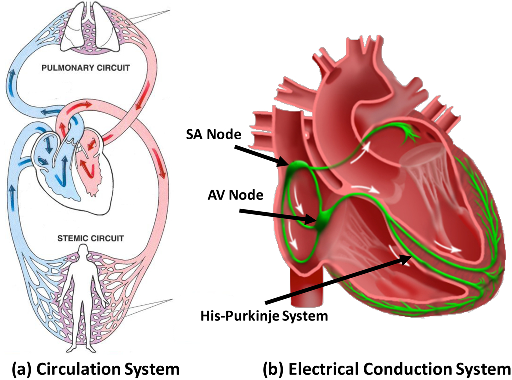
\includegraphics[width=0.9\textwidth]{figs/circulation.pdf}
		
%\vspace{-10pt}
\caption{\small (a) The circulation system. (b) Electrical Conduction system of the heart}
\label{fig:circulation}
%\vspace{-15pt}
\end{figure} 
\subsection{Electrical Conduction System of the Heart}
The oxygen demand of the body changes during different activities. For example, the demand is higher while running and lower while sleeping. To satisfy these demands, the heart muscles in the atria and the ventricles have to contract with certain frequency and in accordance to optimize the \emph{Cardiac Output}, which refers to the volume of blood pumped by the heart per minute (mL blood/min). The coordinated contractions of the heart muscles are governed by the electrical conduction system of the heart (\figref{circulation}.(b)) A \emph{Normal Sinus Rhythm (NSR)} is the healthy heart rhythm which provides efficient blood flow. During a NSR, electrical signals are periodically generated by the \emph{Sinoatrial (SA) node} in the upper right atrium, which acts as the intrinsic pacemaker of the heart. The signals conduct throughout both atria and trigger muscle contractions to push blood into the ventricles. After a long conduction delay at the \emph{AV node} so that both ventricles are fully filled, the signals conduct through fast-conducting \emph{His-Purkinje} system to trigger almost simultaneous contractions of the ventricles and pump blood out of the ventricles. 

Derangement from NSR can result in insufficient cardiac output and thus insufficient oxygen supply to the body and/or the heart itself, which are referred to as \emph{Arrythmia}. Arrhythmia impair the heart's ability to efficiently pump blood and compromise the patient's health. 
Arrhythmia are categorized into so-called \emph{Tachycardia} and \emph{Bradycardia}. Tachycardia features undesirable fast heart rate which can cause inefficient blood pumping. Bradycardia features slow heart rate which results in insufficient blood supply. Bradycardia are due to failure of impulse generation with anomalies in the SA node, or failure of impulse propagation where the conduction from atria to the ventricles is delayed or blocked. 
\subsection{Electrophysiology and Implantable Cardiac Devices}
\label{EP}
The electrical activities of the heart closely couple with the mechanical contractions thus the electrical activities of the heart can be monitored and used to diagnose arrhythmia. The most well-known method is Electrocardiogram (ECG), which measures the integration of electrical activities of the heart measured along different axis on the body surface. The electrical activities can also be directly measured by inserting electrodes through the vein into the heart. The electrodes are placed against the inside heart wall and localized electrical activities can be measured. Physicians can also deliver pacing sequence through the electrodes to explore the heart conditions. This procedure is referred to as Electrophysiological (EP) Testing  (\cite{josephson}) and the signals are referred to as electrograms (EGMs) (\figref{probes}.b). The timing and morphology of the  ECG and EGM signals together are used to diagnose arrhythmia.
\begin{figure}[!t]
\centering
		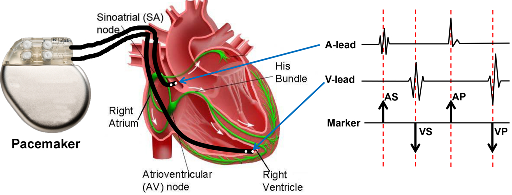
\includegraphics[width=0.9\textwidth]{figs/egm.pdf}
		
%\vspace{-10pt}
\caption{\small (a) Lead placement for a dual chamber pacemaker. (b) Electrogram (EGM) signals measured from pacemaker leads and corresponding internal pacemaker events}
\label{fig:probes}
%\vspace{-15pt}
\end{figure} 

%Implantable pacemakers follow the principle of EP testing. For a dual chamber pacemaker, two leads are inserted into the right atrium and right ventricle, respectively. The pacemaker senses the intrinsic generation and conduction of the electrical signals in the two chambers and deliver electrical pacing when the heart rate and/or atria-to-ventricles conduction interval are abnormal.
The implantable cardiac pacemakers are rhythm management devices designed to treat bradycardia. A typical dual chamber pacemaker has two leads inserted into the heart through the veins which can measure the local electrical activity of the right atrium and right ventricle respectively (\figref{probes}.a). According to the timing between sensed impulses, the pacemaker may deliver electrical pacing to the corresponding chamber to maintain proper heart rhythm.

\section{A Dual Chamber Pacemaker Specification}
In our study, we focus on the implantable pacemaker, which is one of the simpler implantable cardiac devices.
The functionality of a pacemaker is based on the timing of local electrical events, which can be intuitively modeled with timed automata. 
The specifications are based on the algorithm descriptions from Boston Scientific manuals (\cite{compass}) and the functional description released as part of the Pacemaker Challenge (\cite{challenge}). 


The pacemaker is designed for patients with bradycardia (i.e. slow heart rate). Two leads, one in the right atrium and one in the right ventricle, are inserted into the heart and fixed onto the inner wall of the heart. These two leads monitors the local activation of the atria and the ventricles, and generate corresponding sensed events \textsf{(AS, VS)} to its software. The software determines the heart condition by measuring time difference between events and delivers pacing events \textsf{(AP, VP)} to the analog circuit when necessary. The analog circuit then delivers pacing signals to the heart to maintain heart rate and A-V synchrony. In order to deal with different heart condition, pacemakers are able to operate in different modes. The modes are labeled using a three character system (e.g. $xyz$). The first position describes the pacing locations, the second location describes the sensing locations, and the third position describes how the pacemaker software responds to sensing. Here we introduce the widely used DDD mode pacemaker which is a dual chamber mode with sensing and pacing in both atrium and ventricle. 

\begin{figure}[!b]
\center
%\vspace{-10pt}
\includegraphics[width=0.85\textwidth]{figs/PM_timers.pdf}
%\vspace{-10pt}
\caption{Basic 5 timing cycles for a dual chamber pacemaker which include the Lower Rate Interval (LRI),  Atrio-Ventricular Interval (AVI), and Upper Rate Interval (URI). Also included are the blanking intervals, Post Ventricular Atrial Refractory Period (PVARP) and Ventricular Refractory Period (VRP), to inhabit action by the pacemaker.}
\label{fig:PMtimers}
%\vspace{-10pt}t

\end{figure} 
A DDD pacemaker has five basic timing cycles triggered by external and internal events, as shown in \figref{PMtimers}. We decomposed our pacemaker model into five components which correspond to the five timers. $P=LRI\| AVI\| URI\| PVARP\| VRP$. These components synchronize with each other using broadcast channels and shared variables (as shown in \figref{PMdesign}). 

\subsection{Lower Rate Interval (LRI)}
%\vspace{-5pt}
The Lower Rate Interval (LRI) component is shown in \figref{PMdesign}(a). This component defines the longest interval allowed between two ventricular events, thus keeping the heart rate above a minimum value. In DDD mode, the LRI interval is divided into a V-A interval (TLRI-TAVI) and a A-V interval (TAVI). The LRI component maintains a maximum V-A delay while the AVI component maintains a maximum A-V delay so together they maintain the maximum V-V delay. In the LRI component, the clock is reset when a ventricular event \textsf{(VS, VP)} is received. If no atrial event has been sensed \textsf{(AS)}, the component will deliver atrial pacing \textsf{(AP)} after TLRI-TAVI. 

%\vspace{-5pt}
\subsection{Atrio-Ventricular Interval (AVI) and Upper Rate Interval (URI)}
%\vspace{-5pt}
The function of the AVI component defines the longest interval between an atrial event and a ventricular event. If there is no ventricular event \textsf{(VS)}  within TAVI after an atrial event \textsf{(AS, AP)}, and the time since the last ventricular event \textsf{(VS, VP)} is longer than TURI, the component will deliver ventricular pacing \textsf{(VP)}. The URI limits the ventricular pacing rate by enforcing a lower bound on the times between consecutive ventricle events. The UPPAAL design of AVI and URI component is shown in \figref{PMdesign}(b) and (c).%The UPPAAL design of AVI component is shown in 

%\vspace{-10pt}
\subsection{Post Ventricular Atrial Refractory Period (PVARP) and Post Ventricular Atrial Blanking (PVAB)}
%\vspace{-5pt}
Ventricular events, especially Ventricular Pace \textsf{(VP)} are sometimes so strong that the atrial lead can sense the activation as well. This signal may be falsely recognized as an atrial event and disrupt normal pacemaker function. This scenario is called crosstalk and was discussed in our previous work (\cite{vhm_embc11}). In order to prevent this undesired behavior, and filter potential noises, there is a blanking period (PVAB) followed by a refractory period (PVARP) for the atrial events after each ventricular event \textsf{(VS, VP)}. Atrial events during PVAB are ignored and atrial events during PVARP trigger \textsf{AR!} events which can be used in some advanced diagnostic algorithms. The UPPAAL design of PVARP component is shown in \figref{PMdesign}(d).

%\vspace{-10pt}
\subsection{Ventricular Refractory Period (VRP)}
%\vspace{-5pt}
The VRP follows each ventricular event \textsf{(VP, VS)} to filter noise and early events in the ventricular channel which could otherwise cause undesired pacemaker behavior. 

\section{Identify Safety Hazards in the Dual Chamber Pacemaker}
Implantable pacemakers are designed to treat bradycardia by increasing the heart rate with external pacing. Therefore the heart rate should not only be increased to the minimum physiological need, but also should not be increased beyond physiological need. \figref{risk_req} demonstrates two Fault Tree Analysis (FTA) for these two top level hazards. In the remaining chapter we first specify hazards as properties, and use model checking to evaluate whether these hazards have been mitigated by the pacemaker. Then for one of the mitigation algorithm, we examine the mitigation effectiveness and the residue hazard.
\begin{figure}[!t]
		\centering
		\includegraphics[width=0.8\textwidth]{figs/risk_requirements.pdf}
		\caption{\small Sample Fault Tree Analysis of the physiological conditions leading to the lower rate limit and upper rate limits}
		  %\vspace{-15pt}
		\label{fig:risk_req}
\end{figure}

\section{Known Safety Hazards of Dual Chamber Pacemakers}
In this section we introduce two well-studied safety hazards in a basic dual chamber pacemaker design.
Device manufacturers have developed algorithms to mitigate the hazards.
In the following chapters, I will use model-based techniques to identified these safety hazards in the early design stage, and evaluate the effectiveness of the mitigation algorithms developed by device manufacturers.

\subsection{Endless-Loop Tachycardia}
\begin{figure*}
\centering
%		\vspace{-10pt}
		\subfigure [Virtual circuit formed by the pacemaker and the heart] {
				\includegraphics[width=0.4\textwidth]{figs/ELT_str.pdf}
				\label{fig:ELT_demo}
		} 
		\subfigure [Pacemaker trace for ELT initialized by a early ventricular signal]{	
			\includegraphics[width=0.4\textwidth]{figs/ELT.pdf}
			\label{fig:ELT}
		}
%		\vspace{-10pt}
	\caption{Endless Loop Tachycardia case study demonstrating the situation when the pacemaker drives the heart into an unsafe state \cite{vhm_iccps11}}
%\vspace{-15pt}
\end{figure*}


The AVI component of a dual-chamber pacemaker introduces a virtual A-V conduction pathway. This forms a timing loop with the intrinsic (physiological) A-V conduction pathway (see \figref{ELT_demo}). A Premature Ventricular Contraction (PVC), i.e. an early extra beat in the ventricles, may trigger another ventricular event (VS) and initiate a V-A conduction through the intrinsic pathway (Marker 1 in \figref{ELT}). The pacemaker registers this signal as an Atrial Sense (AS) (Marker 2 in \figref{ELT}). This event triggers a VP after TAVI, as if the signal conducts through the ``virtual" A-V pathway (Marker 3 in \figref{ELT}). We call it ``virtual" pathway as the ``conduction" delay is fulfilled by a timer in the pacemaker instead of a physical signal propagation along the heart tissue. The VP will trigger another V-A conduction and this VP-AS-VP-AS looping behavior will continue (see \figref{ELT}). The interval between atrial events is TAVI plus the V-A conduction delay, which is normally shorter than the delay between intrinsic heart beats, thus driving the ventricular rate as high as the Upper Rate Limit. During ELT, the heart rate is not only high, but also fixed, which is an unsafe scenario.

\subsection{Atrial Tachycardia Response}

Supraventricular Tachycardia (SVT) is an arrhythmia with an abnormally fast atrial rate. %\figref{SVT} is a series of simulation results for closed-loop interaction between a heart model with SVT and the pacemaker model. The atrial and ventricular channels show electrogram inputs to the pacemaker and the pacemaker channel shows the corresponding events received and generated by the pacemaker software, \cite{vhm_embc11}.
Typically, in a heart without pacemaker, the AV node, which has a long refractory period, can filter most of the fast atrial activations during SVT, thus the ventricular rate remains relatively normal. \figref{SVT_none} demonstrates a pacemaker event trace during SVT, with a pacemaker in ODO mode, which just sensing in both channels. 
As there is no pacing in ODO mode, the heart is in open-loop with the pacemaker. In this particular case, every 3 atrial events (AS) correspond to 1 ventricular event (VS) during SVT. 
As an arrhythmia, SVT is still considered a safe heart condition since the ventricles operate under normal rate and still maintain adequate cardiac output. 

However, in the closed loop case with the DDD pacemaker, the AVI component of a dual chamber pacemaker is equivalent to a virtual pathway in parallel to the intrinsic conduction pathway between the atria and the ventricles. The pacemaker tries to maintain 1:1 A-V conduction and thus increases the ventricular rate inappropriately to match the atrial rate.  This is known as Pacemaker Mediated Tachycardia (PMT) as the heart would have been safe without the pacemaker and its virtual pathway. \figref{SVT_DDD} shows the pacemaker trace of the same SVT case with DDD pacemaker. Although half of the fast atrial events are filtered by the PVARP period ([AR]s), the DDD pacemaker still drives the closed-loop system into 2:1 A-V conduction with faster ventricular rate. Maintaining A-V delay is less important than maintaining an appropriate ventricular rate. The DDD pacemaker violates a higher priority requirement in order to satisfy a lower priority requirement, which is inappropriate.
\begin{figure*}[!t]
\centering
		\subfigure [\small]{			
		\includegraphics[width=0.5  \textwidth]{figs/SVT_none.pdf}
		\label{fig:SVT_none}
		} 
%	\hspace{.1in}%
		
		\subfigure [\small] 
		{
		\includegraphics[width=0.5\textwidth]{figs/SVT_DDD.pdf}
		\label{fig:SVT_DDD}
		} 
\caption{\small Benign open loop case: SVT without a pacemaker or with a pacemaker in sense-only mode (ODO) (b) Dangerous closed-loop-case SVT with DDD pacemaker which tries to match the fast atrial rate with a corresponding (and dangerous) fast ventricular rate.}
\end{figure*} 

\section{Discussion}
Implantable cardiac devices such as implantable pacemakers are typical autonomous medical devices.
Although the functionality is relatively simple, pacemakers illustrate the three challenges discussed in the introduction very well.
In the following chapters, I will demonstrate the use of different model-based techniques to provide safety and efficacy confidence to the pacemaker design.



\chapter{Theme 1: Modeling the Physiological Environment}

Closed-loop medical devices such as the implantable cardiac pacemaker and defibrillator are designed to operate autonomously and interact with the human body to maintain and improve the physiological conditions of the patients. To evaluate the device within the closed-loop context of the human body, the knowledge of the physiological contexts (e.g. patient arrhythmia, physical activity) and the signals by which the device interacts with the organ(s) to manage the condition is essential. By constructing physiological models and encoding physiological requirements, our goal is to evaluate the safety and efficacy of the device therapy across a range of physiological conditions. 

Consequently, it is important to model the physiological environment of the device such that details unrelated to the interaction between the device and the human are abstracted away, while essential information required to differentiate different patient conditions are maintained. As we will see, to validate the device operation across a range of physiological conditions and for a set of safety and efficacy properties, a family of models are needed which refine the closed-loop context to appropriately express the condition to be verified.

%\newpage
%\begin{itemize}
%\vspace{-5pt}
%\item How does the device interact with the physiological environment?
%\vspace{-5pt}
%\item What details must the physiological environment models capture?
%\vspace{-5pt}
%\item What are the different modeling philosophies when developing environment models for testing and for model checking?
%\end{itemize}

Models, especially models of the human physiology, which span a large spectrum of scale and complexity, should be designed in accordance with their respective applications. Each application of the environment model has a different focus and has distinct modeling requirements which influence the model complexity and model identifiability.

\textbf{Model complexity:} How much detail should the physiological models have, in order to unambiguously describe a physiological behavior? In particular, if the model checker returns an execution trace as counter-example, how much details should the physiological model have so that the execution traces can be interpreted by domain experts? 	

\textbf{Model Identifiability} is a metric for the feasibility of identifying model parameters from data. There are two methods for model construction: non-parametric modeling in which no prior knowledge is assumed and the model construction is purely data-driven; and parametric modeling in which domain knowledge of the physiological conditions is taken into account. For example, to model the electrophysiological activity of the heart, there is abundant literature describing the phenomena of individual arrhythmia, which makes parametric modeling of the environment favorable.

%%It affects the validity of the model which is a key element for closed-loop verification. Model identifiability is generally affected by the model complexity and the availability and quality of clinical data. 

%%The complexity requirements of an environment model is usually determined by 1) The complexity of the interactions between the environment model and the system model and 2) The complexity of the environment condition specified in the physiological requirements.

In the following sections, we introduce the physiological contexts within which the implantable pacemaker operates, and proceed to construct a heart model structure for closed-loop validation of the pacemaker. Note that for two different applications, i.e. model checking of the device model in the loop and functional testing of the actual device in the loop, models are constructed differently as we address their respective requirements for environment models. 



\begin{figure}[!t]
\centering
		\includegraphics[width=0.9\textwidth]{figs/models.pdf}
		
%\vspace{-10pt}
\caption{\small Physiological models of the heart from different perspectives}
\label{fig:models}
%\vspace{-15pt}
\end{figure} 
\section{Physiological Models of the Heart}
To study the mechanisms of heart diseases and their effects on cardiac output, different physiological models of the heart have been developed. \figref{models} illustrates several aspects that these models capture. With the development of the imaging techniques like MRI, detailed anatomical structures of the heart can be modeled and studied (\cite{geometric}). These models are fundamental in other modeling aspects as well, as the anatomy of the heart dictates the electrical and mechanical behaviors of the heart. \figref{models}.(a) shows models for heart muscle fiber orientations by \cite{fiber}. With anatomy models the electrical and/ or mechanical properties of the heart can be studied. \figref{models}.(b) illustrate a model of blood flow within the ventricles (\cite{bloodflow}). Electrical properties of the heart at cellular level has been modeled (\cite{cellular}) and by combining these cellular models with the structural models, the electrical activities of the whole heart are studied, especially the mechanism of different arrhythmia (\cite{natalia},~\cite{Grosu_MHA},~\cite{Grosu_wave}). Intrinsic heart rate variability has been modeled to synthesize optimal control of pacemaker pacing. (\cite{Bogdan}) Abstraction of the electrical cellular model has also been attempted by \cite{Grosu_abstract} to reduce model complexity without sacrificing accuracy. The electrical properties and the mechanical properties of the heart are closely coupled. Models combining both of these aspects are also developed to study the effects of different arrhythmia on cardiac outputs (\cite{natalia},~\cite{eletro_mechanical}).

\section{EP Heart Model Structure for Closed-loop Validation of Implant-able Cardiac Devices}
Models should be developed according to their applications. The aforementioned models of the heart are mostly used for understanding the mechanisms of different heart diseases. Physiological models developed for closed-loop evaluation of medical devices should have the following considerations:\\
\textbf{C1. Interfacing with the device: }The model should be able to generate physiological signals that the device sense from the real physiological entities. And the model should be able to take device output as input and change its states accordingly. Model complexity should also be adjusted according to the device interface to hide unnecessary details.\\
\textbf{C2. Differentiate different physiological conditions: }To evaluate the safety and effectiveness of the device, the device has to be evaluated under certain physiological conditions specified by the requirements. For example, the pacemaker is supposed to maintain proper heart rate during Bradycardia. The model should be expressive enough to be able to differentiate the physiological condition (Bradycardia in the example) from other conditions. Failing to do so may result in false-positives or false-negatives in the evaluation result. \\
\textbf{C3. Physiological/logical interpretation of model states: } In closed-loop evaluation we are checking the device safety and effectiveness against the physiological requirements. However, due to the limited interface (e..g two leads for a dual chamber pacemaker) it is always difficult to determine only from an execution trace that the therapy is safe and effective. Therefore, being able to provide physiological meanings to the states of the model also allows us to interpret the closed-loop execution more accurately, thus reducing the number of physiologically impossible executions during the evaluation. To satisfy these requirements, the model structure of these physiological models should base on physiological or clinical first principles so that states and state transitions of the closed-loop executions can be explained with physiological language. \\%One advantage of closed-loop evaluation over open-loop evaluation is the capability to provide physiological/logical interpretation of an execution trace. With this advantage we are able to identify and reduce the number of physiological-impossible executions by examining the state of the model, so that the evaluation can focus on physiological-possible executions. This requires the model first-principle\\
\textbf{C4. Available patient data: } In closed-loop evaluation, physiological models are developed to represent certain physiological condition across a population of patients or even a particular patient. The model parameters must be identified so that the behaviors of the models match the behaviors of the patients (groups).  Due to the limited sensing capability of closed-loop medical devices, the obtained data is sparse. i.e. we can not put a sensor on every tissue region of the heart. Therefore the complexity of the model should be in accordance with the available data to avoid \emph{over-fitting}, which occurs when a model has too many parameters relative to the number of observations, and this can introduce errors during prediction. 

The electrophysiological models mentioned in the last section (\cite{natalia,Grosu_MHA}) satisfy C1-C3. However, the parameter space of these models are too large (10+ parameters for each cellular model multiplied by $10^5$ of elements) which not only increase simulation complexity, but also impossible to identify due to lack of data. As introduced in Section \ref{EP}, the pacemaker has only two leads at fixed locations and only use timing between local activation events for diagnosis. These models with high spatial fidelity possess details that can be abstracted without sacrificing the three considerations.

Electrophysiology testing (EP testing) has been an active clinical field to diagnose and treat arrhythmia with minimal-invasive procedures. During an EP testing procedure, the physicians diagnose heart conditions by examining the patterns and intervals of local electrical activations (temporal) measured from electrodes placed into different locations of the heart (spatial). EP testing is the perfect modeling level for closed-loop evaluation of implantable cardiac devices because: 1) it is the basis of implantable cardiac devices (C1), 2) physicians can use EP testing to diagnose most arrhythmia thus distinguish them (C2,C3), 3) there are abundant patient data available (C4). 

In the remaining chapter we will introduce our heart modeling efforts based on EP testing, and model adaptation for two different applications of closed-loop evaluation of implantable cardiac devices.
%\section{Heart Models for Pacemaker Interaction}
%The heart generates electrical impulses to maintain the heart rate appropriate for the physiological needs. These impulses conduct through the heart, triggering coordinated muscle contractions which pumps blood to the rest of the body. The underlying pattern and timing of these impulses determines the heart's rhythm and is key to proper heart function. Derangements in this rhythm are referred to as \emph{arrhythmia}, which 



%\subsection{Electrical conduction system of the heart}
%Heart tissue with different timing parameters form the electrical conduction system to ensure coordinated contraction of the heart. First, specialized tissue at the Sinoatrial (SA) node periodically and spontaneously self-depolarizes. This is controlled by the nervous system and the SA node is the primary and natural pacemaker of the heart. The activation signal then travels through both atria, causing contraction and pushes blood into the ventricles. Then the activation is delayed at the Atrioventricular (AV) node which allows the ventricles to fill fully. The fast-conducting His-Purkinje system then spreads the activation signal within both the ventricles. The simultaneous contraction of the ventricle muscles will push the blood out of the heart.
%\begin{figure*}[!t]
%\centering
		%\subfigure [\small]{			
		%\includegraphics[width=0.3  \textwidth]{figs/probes.png}
		%\label{fig:probes}
		%} 
%
		%\subfigure [\small] 
		%{
		%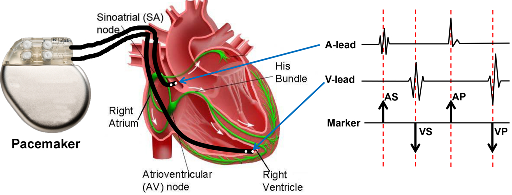
\includegraphics[width=0.2\textwidth]{figs/egm.png}
		%\label{fig:egm}
		%} 
%%\vspace{-10pt}
%\caption{\small (a) Node automaton. Dotted transition is only valid for pacemaker tissue like SA node; (b) Path automaton; (c) Model of the electrical conduction system of the heart using a network of node \& path automata~\cite{vhm_ecrts10}.}
%%\vspace{-15pt}
%\end{figure*} 

%\section{Electrophysiological Testing}
%\Hao{A figure for heart and pacemaker}

%\chapter{Modeling the Physiological Environment}
%\begin{itemize}
	%\item How to encode domain knowledge of the physiological environment into models?
    %\item What are the applications that the models will be used?
    %\item What are the differences in terms of environment models between model checking and simulation?
    %\item How to balance complexity and expressiveness of the model?
%\end{itemize}

%In the following sections, we demonstrate how to construct heart models for closed-loop verification of implantable pacemaker. Note that for two different applications the models are constructed differently as we address their respective requirements for environment models. 


%\begin{itemize}
	%\item Why the models at this level have to be deterministic? Where can they be used?
    %\item How electrophysiology reflects the functions of the heart?
    %\item How to encode these knowledge into models?
    %\item Why VHM has the right level of details for pacemaker verification?
    %\item How VHM interacts with pacemaker?
    %
%\end{itemize}
%During closed-loop testing, the devices interact with the environment (or its models) under different environmental conditions. The closed-loop executions are monitored and violations of safety and efficacy requirements are reported. In model-based closed-loop testing, the environment models are expected to mimic the behaviors of actual environment and its interaction with the device. Thus, the environment models are in general deterministic so that the execution traces are reproducible and are able to mimic different arrhythmia. Complex dynamics during state transitions also need to be captured to validate violations within longer executions traces. 

\subsection{Modeling Philosophy}
As the pacemaker can only sense and actuate from two locations within the heart, only structures and parameters that affect inputs to the pacemaker are needed. Since the two leads are fixed, the accurate spatial locations of different heart anatomical structures are not necessary. Instead, the topology of the electrical conduction system of the heart is more important. 


\begin{figure}[!t]
\center
%\vspace{-10pt}
\includegraphics[width=0.7\textwidth]{figs/refractory.png}
%\vspace{-10pt}
\caption{(a) The generation of Action potential; (b) Action potential; (c1) The second activation arrived during ERP; (c2) Arrived during RRP; (c3) Arrived after refractory.}
\label{fig:refractory}
%\vspace{-10pt}
\end{figure} 
\subsection{Timing Behaviors of Cellular Electrophysiology}
The contraction of heart muscles is triggered by external voltage applied to the tissue. After the activation, a transmembrane voltage change over time can be sensed due to ion channel activities, which is referred to as an Action Potential (\figref{refractory}(a)). The upstroke of the action potential is called depolarization, during which the muscle will contract. The voltage change caused by the depolarization will depolarize the tissue nearby, which causes an activation wave across the heart. After the depolarization there is a refractory period during which the tissue recovers to the pre-excitation state and the voltage drops down to the resting potential. The refractory period can be divided into \emph{Effective Refractory Period (ERP)} and \emph{Relative Refractory Period (RRP)} (\figref{refractory}(b)). During ERP, the tissue cannot be depolarized due to the lack of charge. As a result, the activation wave will be "blocked" at the tissue during ERP (\figref{refractory}(c1)). During RRP, the tissue is partially recovered and the tissue can be depolarized. However, the new action potential generated by the depolarization will have different morphology (e.g. attenuated in magnitude and duration), thus affecting the refractory periods of the tissue and conduction delay of the activation wave (\figref{refractory}(c2)). \figref{refractory}(c1)-(c3) show the action potential shape change and corresponding timing change in refractory periods when the tissue is activated at time stamp $t1$, $t2$, $t3$ after the initial activation $t0$. 

\subsection{Heart Model Components}
We introduce the model components that can be used to configure heart models corresponding to different heart conditions. As discussed earlier, the action potential of a heart tissue has 3 timing periods during which the tissue responds to external electrical stimuli differently. We use an extended timed-automata formulation (\cite{timed_automata}) to model the timing behaviors of a heart tissue during each cycle. 

\textbf{Node Automata:} We refer to the tissue model as \emph{node automaton} and \figref{automata}.(a) shows the structure of a node automaton $i$. 3 states correspond to the timing periods of the action potential. From \textsf{Rest} state, the node can either self-activate or get activated by external stimuli (Act\_node) and go to \textsf{ERP} state. During \textsf{ERP} state the node does not respond to external stimuli (blocked). During \textsf{RRP} state, the node can still be activated and go to \textsf{ERP} state, however the ERP period and the conduction delay of the tissue are affected by the "earliness" of the activation arrived during the RRP period, which is tracked by a shared variable $C(i)$. The new ERP period is determined by a function over clock value $g(f(t))$ which mimics the beat-to-beat dynamics described in \cite{josephson}. The function $g$ and $f$ are given by:
\begin{equation} \label{factor}
						f(t) = 1-t/Trrp
						\end{equation}
and
%  The AV node has a different profile than the other tissue. The ERP period increases rather than decreases when activated during its RRP (~\cite{josephson}).
\begin{equation} \label{earliness_noAV}
						g(x) = \left\{
						\begin{array}{lr}
						
						T_{min}+(1-(1-x)^3)\cdot (T_{max}-T_{min}), i=AV\\
						T_{min}+(1-x^3)\cdot (T_{max}-T_{min}),i\neq AV
			
						
						\end{array}
						\right.
						\end{equation}  
where $T_{min}$ and $T_{max}$ are the minimum and maximum value for \emph{Terp} of the tissue.
\begin{figure}[!t]
%\centering
		%\subfigure [\small]{			
		\includegraphics[width=\textwidth]{figs/automata.pdf}
		%\label{fig:node_automata}
		%} 
%%	\hspace{.1in}%
		%\subfigure [\small] 
		%{
		%\includegraphics[width=0.32\textwidth]{figs/path.pdf}
		%\label{fig:path_automata}
		%} 
		%\subfigure [\small] 
		%{
		%\includegraphics[width=0.25\textwidth]{figs/gen_setup.png}
		%\label{fig:general_setup}
		%} 

%\vspace{-10pt}
\caption{\small (a) Node automaton: The dotted transition is only valid for tissue (like SA node) that can be activated by an external trigger; (b) Path automaton modeling the electric conduction and propagation between two node automata; (c) Electrical conduction system of the heart; (d) Model of the electrical conduction system of the heart using a network of node \& path automata ~\cite{VHM_proc}.}\label{fig:automata}
%\vspace{-15pt}
\end{figure} 

Due to the limited number of observable points within the heart, modeling the electrophysiological behavior of every tissue of the heart and its full anatomy is unnecessary and unfeasible. In our heart models, only self-activating tissue and key hubs of the electrical conduction system are modeled as node automata. 

\textbf{Path Automata:} The electrical conduction through the tissue between nodes are abstracted using \emph{path automata}. The path automata can be used to represent structural or topological (functional) electrical connections between nodes. \figref{automata}.(b) shows a path automaton connecting node a and b.

The initial state of a path automaton is \emph{Idle}, which corresponds to no conduction. The states corresponding to the two conduction directions are named after the physiological terms: Antegrade (Ante) and Retrograde (Retro). These states can be intuitively described as forward and backward conductions. If path actuation \emph{Act\_path} event is received from one of the nodes connected to it, there is a transition to \emph{Ante} or \emph{Retro} state based on the activation source in the path automaton. At the same time, the clock invariant of the state is modified according to the shared variable \emph{C(a/b)}. This corresponds to the change of the conduction delay that is caused by the early activation. Similar to node automaton, the changing trend is extracted from clinical data and the function $h$ is defined as:
\begin{equation} 
						h(c) = \left\{
						\begin{array}{lr}
						
						path\_len/v\cdot (1+3c), i=AV\\
						path\_len/v\cdot (1+3c^2), i\neq AV
						\end{array}
						\right.
						\end{equation}
where $path\_len$ denotes the length of the path and $v$ is the conduction velocity.

After \emph{Tante} or \emph{Tretro} time expires, the path automaton sends out \emph{Act\_node(b)} or \emph{Act\_node(a)} respectively. A transition to \emph{Conflict} state occurs followed by the transition to \emph{Idle} state. The intermediate state \emph{Conflict} is designed to prevent back-flow, where the path is activated by the node \emph{b} it has just activated. If during \emph{Ante} or \emph{Retro} state another \emph{Act\_path} event is received from the other node connected to the path automaton, a transition to \emph{Double} state will occur, corresponding to the two-way conduction. In this case, the activation signals eventually cancel each other and the transition to \emph{Idle} state is taken.

\subsection{Modeling the Heart's Electrical Conduction System}
The node and path automata are the basic building blocks for EP heart modeling. Hearts with different conditions are modeled by using different conduction topologies with appropriate timing parameters for each node and path automata. \figref{automata}.(d) shows one such topology of a network of node and path automata.
\begin{figure}[!t]
\center
%\vspace{-15pt}
		\includegraphics[width=0.7\textwidth]{figs/fig7.png}
%\vspace{-10pt}
\caption{The influence of conduction velocity and probe configuration on the EGM morphology. The left columns show the placement of probes in relation to the path; the right columns show the functional EGM.}
\label{fig:egm_s}
%\vspace{-15pt}
\end{figure}
\section{Interaction with the Heart Model}
In this section, we first introduce a probe model we developed to generate synthetic EGM signals from the EP heart model.
We then use two case study to demonstrate that the probe model enables the EP heart model to evaluate device malfunctions due to sensing errors.
\subsection{Probe Model for Synthetic EGM Generation}
In EP testing and during pacemaker implantation, the local electrical activities, measured as electrogram (EGM) signals, are used to diagnose heart conditions. During heart model construction, we can assign a node automaton at electrode locations and the transitions to the ERP state can be used to represent the local activation events. In a more general setup where electrodes are assigned anywhere within the heart model, a probe model is designed to generate synthetic EGM signals using spatio-temporal information from the proximity to the network of node and path automata. 
According to \cite{recording}, a potential difference is generated when the activation wavefront passes by the electrode. 
The locations of the activation wavefronts are calculated from the locations of the path automata and their current timer values. 
The amplitude of EGM decreases when the activation wavefront moves away from the probe. 
We assume the decrease factor is a function related to the distance between the activation wavefront and the probe. 
The potential difference caused by an activation wavefront to a probe is the signal strength of the path multiplied by the decrease factor. 
The amplitude of EGM from a probe is the sum of potential differences caused by all activation wavefronts. The bipolar EGM is the subtraction between two unipolar EGMs. 
\figref{egm_s} shows that this probe model captures timing properties of EGM and the functional shape of the EGM impulses. The probes can be placed anywhere within the heart model and generate clinically-relevant EGMs. 

\begin{figure}[!t]
\center
%\vspace{-15pt}
		\includegraphics[width=0.98\textwidth]{figs/modeling_heart.pdf}
%\vspace{-10pt}
\caption{The heart model was developed in Matlab/Simulink and code was automatically generated to operate on an FPGA platform for platform-level testing.}
\label{fig:modeling_heart}
%\vspace{-15pt}
\end{figure}

\begin{figure}[t]
\center
\vspace{-10pt}
		\includegraphics[width=0.6\textwidth]{figs/crosstalk_all.pdf}
%\vspace{-20pt}
\caption{Crosstalk between pacemaker leads with high sensitivity in the ventricle, adjusted sensitivity and ventricular safety pacing}
\label{fig:crosstalk}
%\vspace{-15pt}
\end{figure}
With the sensing model, the heart model structure can be used to identify safety hazards caused by sensing errors.
\subsection{Pacemaker Oversensing and Crosstalk}
Oversensing is a general term for inappropriate sensing caused by noise or far-field signals. It's very common among pacemaker malfunctions and it may result in failure to pace (\cite{med2, leads}), competitive pacing and inappropriate therapy. Crosstalk is a special case for oversensing which occurs when the pacemaker stimulus in one chamber is sensed in the other chamber. It happens when two leads are close to each other or pacing signal in the other chamber is too strong. It is common that the ventricular lead is placed in the right ventricle outflow tract, which is close to the atrium (\cite{icd}). \figref{crosstalk}(a) shows simulated EGMs from a patient with bradycardia and complete heart block. During atrial pacing (AP), the pacing signal is sensed by the ventricular lead 53 ms after the AP. (Marker 1) It is treated as ventricular sense (VS) signal and thus inhibits the subsequent ventricular pacing (VP). This is indicated by no QRS-wave in the ECG channel. (Marker 2) For a patient with complete heart block this will cause dangerous ventricular asystole, meaning a long time without ventricular events.  

Increasing the sensing threshold of the ventricular channel can prevent false sensing. In \figref{crosstalk}(b), the small signals in ventricular EGM are ignored and ventricular pacing are successfully delivered. 


%%%%%%%%%%%%%%%%%%%%%%%%%%%%%%%%%%%%%%%%%%%%%%
\begin{figure}[t]
\centering
\vspace{-10pt}
		%\subfigure [\small]{
		\includegraphics[width=\textwidth]{figs/dislodge_all.pdf}
		%} 
		%\subfigure [\small]{
		%\includegraphics[width=0.36\textwidth]{figs/dislodge_norm.pdf}
		%\label{fig:dislodge_norm}
		%} 
		%\subfigure [\small] 
		%{
		%\includegraphics[width=0.36\textwidth]{figs/dislodge_new.pdf}
		%\label{fig:dislodge}
		%} 
%\vspace{-5pt}
\caption{\small (a) Dotted line shows the location where the atrial lead should be (b) Pacemaker function before lead dislodge. (b) Pacemaker function after lead dislodge}
		\label{fig:dislodge_all}

%\vspace{-15pt}
\end{figure} 
%%%%%%%%%%%%%%%%%%%%%%%%%%%%%%%%%%%%%%%%%%%%%%


\subsection{Lead Displacement}
Lead displacement affects many patients and can result in inappropriate or ineffective therapy. \figref{dislodge_all}. (b) shows the simulation result for the pacemaker function when the leads are in their designated location. From the figure we can observe: 1) Each P-wave is initialized by an Atrial Pace signal. 2) Each QRS complex is initiated by a ventricular pacing signal. 3) The interval between AP and VP is 150 ms, which matches the programed AVI period.

%%%%%%%%%%%%%%%%%%%%%%%%%%%%%%%%%%%%%%%%%%%%%%
 %\begin{figure}
%\center
%\includegraphics[width=0.7\textwidth]{figs/race_cond.pdf}
%\caption{Dotted line shows the location where the atrial lead should be}
%%\vspace{-15pt}
%\label{fig:race_cond}
%\end{figure}
%%%%%%%%%%%%%%%%%%%%%%%%%%%%%%%%%%%%%%%%%%%%%%

One common case for lead dislodge is shown in \figref{dislodge_all}.(a), where the atrial lead has fallen into the right ventricle outflow tract. In this case the atrial lead senses from the ventricle rather than atrium and atrial pacing will initiate a ventricular event. \figref{dislodge_all}.(c) shows the simulated EGMs in this case. The figure reveals several facts: 1) No P wave is sensed or tracked (Marker 1). 2) Atrial Pace initiates an abnormal, wide QRS which is then sensed by the ventricle lead (Marker 2). 3) Intermittent appearance of VP on QRS 110 ms after the AP. The ventricular lead can receive signal from: 1) pacing signal sent from the atrial lead, 2) the intrinsic A-V conduction path. The two paths are shown in \figref{dislodge_all}.(a) and form a timing race condition. When the signal from the atrial lead arrives the ventricular lead first, it will trigger VS. If the intrinsic signal arrives the ventricular lead during the VSP sensing window (defined in previous section), it will trigger VSP. Although the pacing is 'safe' because the pacing is early enough to avoid the vulnerable refractory period, the damage caused by pacing on depolarized tissue is currently a matter of much investigation.\\



\section{Heart-on-a-Chip Platform}
Platform testing remains the primary means to verify and validate device software. Currently testing is performed by feeding recorded open-loop heart signals to the device and evaluating the device output. Consequently, the change in the state of the heart condition, in response to device output, is not taken into account. Thus, device malfunctions involving state changes due to multiple closed-loop interactions will not be captured during open-loop testing. 

To this effect, the heart model described above is also implemented on hardware platform (\figref{modeling_heart}) for closed-loop testing. Since each heart model is a network of node and path automata running concurrently, we implemented the heart model on an FPGA, so that increasing in the number of nodes and paths would not affect real-time constraints. The second generation heart model implementation has been implemented on a lower cost fast micro-controller platform. The fast clock ensures that executions of all nodes and paths can be finished within 1ms. The Heart-on-a-Chip platform includes a heart model implementation which is able to represent common heart conditions such as bradycardia, tachycardia, heart block, etc (for mode details refer to \cite{VHM_proc}). The parameters of the heart model can be changed at run-time by either switching among pre-defined parameter sets, or sending values directly to the model through a user interface in Matlab. A monitoring system observes logical interactions between heart model and the pacemaker and checks them against safety invariants at run-time. 

As shown in (\figref{HOC}), with an analog interface the heart model can interact with a commercial pacemaker in real time. Our analog interface uses an optical isolation circuit to separate the pacemaker circuit and the heart implementation. Signals generated from the heart are attenuated to the appropriate level to interact with a Boston Scientific pacemaker and analog pacing signals are converted to pacing events received by the heart model. 

\begin{figure}[!b]
\center
%\vspace{-15pt}
		\includegraphics[width=0.8\textwidth]{figs/PVS.pdf}
%\vspace{-10pt}
\caption{Heart-on-a-Chip testbed for real-time closed-loop testing of the pacemaker or model of the pacemaker with the heart model on the hardware platform}
\label{fig:HOC}
%\vspace{-15pt}
\end{figure}

% \subsubsection{Abstracting Beat-to-beat Dynamics}
% \subsubsection{Abstracting Conduction Delays with Path}
% \subsubsection{Merging Activation-generating Nodes}
% \subsubsection{Replace ERP Blocking With Non-deterministic Conduction}
% \subsubsection{Replace }





\include{C}



%%%%%%%%%%%%%%%%%%%%%%%%%%%%%%%%%%%%%%%%%%%%
%%%%%%%%%%%%%%%%%%%%%%%%%%%%%%%%%%%%%%%%%%%%

\chapter{Theme 2: Closed-loop Model Checking for Implantable Pacemaker}
\label{ModelChecking}
%There are two categories of device bugs: 
%1) the device may fail to conform to its \emph{specifications}, that is, the prescription of how it should react to certain inputs.  
%2) the device may fail to improve the conditions of the patient as promised, even if it conforms to its specifications. 
%The desired physiological conditions that the closed-loop system should achieve are captured in the \emph{physiological requirements}; for example, for a pacemaker, the heart rate should always be maintained above a certain threshold. 
%
%Bugs in the first category (non-conformance to specification) can be detected via systematic and extensive open-loop testing in which a set of input sequences is fed to the device, and its output is compared with the expected output.
%Bugs in the second category (violation of physiological requirements), on the other hand, require the interaction within the \emph{closed-loop system}, which consists of the device and its environment.
%For instance, the pacemaker and the heart as its environment. 
%In the medical device industry, closed-loop verification of the physiological requirements is mostly performed in terms of clinical trials, in which the actual devices are implanted in human subjects over an extended duration.
%Unfortunately, because of the extremely high cost of clinical trials (several million dollars and spanning several years,~\cite{trialcost}), the amount and variety of human subjects during the clinical trials are limited, which reduces the opportunity to find bugs. 
%Moreover, clinical trials are often conducted at the final design stage. Fixing bugs at this stage is very costly.

Model checking is a technique in which the state space of the model under investigation is automatically and exhaustively explored to identify executions or states that violate specified properties. 
Violations of the properties are returned by the model checkers as \emph{counter-examples}, which can be used by designers to revise the design. 
In this chapter, model checking is used to evaluate an early design of a dual chamber pacemaker. 
More specifically, model checking is used to identify known and unknown physiological hazards induced by implantable pacemakers (e.g. when the pacemaker provides inappropriate therapy which drives the heart to an unsafe state).  

The chapter is organized as follow: first the basis for timed-automata formalism is introduced.
The dual chamber pacemaker specification introduced in Chapter 2 is implemented in model checker UPPAAL.
The heart model structure in Chapter 3 is adjusted for closed-loop model checking of the pacemaker model.
An abstraction tree of heart models is constructed to capture heart behaviors for different heart conditions and provide physiological contexts to counter-examples.
Finally the abstraction tree is used to check safety and efficacy properties of the pacemaker model, as well as the effectiveness of additional algorithms developed to mitigate two known safety hazards. 
We demonstrated that with appropriate models of the physiological environment, closed-loop model checking is capable of finding safety and/or efficacy violations within autonomous medical devices during device development.

\section{Related Work}
Jee et. al present a safety assured development approach of real-time software using pacemaker as their case study in \cite{Jee}. They formally model and verify a single chamber VVI pacemaker using UPPAAL and then implement it and check the preservation of properties transferred from model to implementation code. 

Chen et. al \cite{Marta} extended our verification work \cite{TACAS12}. They developed a hybrid heart model which is able to simulate action potential at tissue level. The model is a more refined model than our Virtual Heart Model \cite{VHM_proc}, with linear dynamics on each state of the heart tissue. They also developed a probability model to simulate natural pacemaker function. They then used the combined heart model for quantitative verification of the pacemaker. However, since the pacemaker only sense the timing of the heart tissue activation, their hybrid extension for action potential does not bring much benefit but increased model complexity dramatically. As a result, they have to use bounded model checking thus sacrificed accuracy.

Tuan et. al propose an RTS formal model for pacemaker and its environment and verified it against number of safety properties and timed constraints using the PAT model checker \cite{Tuan}. They have modeled the pacemaker for all 18 operating modes as described in Boston scientific, but their work lacks specification and analysis of complex behaviors of the pacemaker, such as mode-switch.

Wiggelinkhuizen uses mCRL2 and UPPAAL to formally model the pacemaker from the firmware design of Vitatron's DA+ pacemaker \cite{Wigg}. Two main approaches have been used to investigate the feasibility of applying formal model checking to the design of device firmware. The main approach consists of verifying the firmware model in context of a formal heart model and a formal model of a hardware module which fails for high heart rates because of the state explosion. Another approach is to verify a part of firmware design which was feasible and was able to detect a known deadlock rather soon.

Macedo et. al have developed a concurrent and distributed real-time model for a cardiac pacemaker through a pragmatic incremental approach \cite{Macedo}. The models are expressed using the VDM and are validated primarily by scenario-based test, where test scenarios are defined to model interesting situations such as the absence of input pulses. The models cover 8 modes of pacemaker operation.

Gomes et. al present a formal specification of pacemaker system using the Z notation in \cite{Gomes}. They have also tried to validate that the formal specification satisfies the informal requirements of Boston Scientific by using a theorem prover, ProofPower-Z. They have partially checked the consistency of their specification through reasoning. No validation experiment regarding safety conditions were performed yet.

Mery et. al in \cite{Mery}, formally model all operational modes of a single electrode pacemaker system using event-B and prove them. They use an incremental proof-based approach to refine the basic abstract model of the system and add more functional and timing properties. They use the ProB tool to validate their models in different situations such as absence of input pulses. \\



%Due to the curse of dimensionality as models get more complex, and hence the large computational cost, there are usually restrictions on the formalism and the complexity of the models under investigation. Using abstract models of the actual system adds the responsibility of proving the conformance between the abstract model and the real system. Assumptions made during abstractions may also introduce false-positives and/or false-negatives into the model checking results. Back in Chapter 2, we introduced a set of heart models with different abstraction levels, that can be used to cover behaviors of physiological conditions using non-determinism. In Chapter 4, we then modeled a dual chamber pacemaker algorithm using timed-automata without doing abstractions. In this chapter, we use model checker UPPAAL to evaluate the pacemaker model against safety properties under different heart conditions captured by the heart models. Techniques to eliminate false-positives by refining the heart models are also discussed. We will try to answer the following questions:


%            \item What are the effects of adding new features to the software? Can they disrupt the safety properties that the previous device hold?

%In closed-loop model checking, there is only one device model. 
%However there can be a large number of environmental conditions which require different models to represent them. For instance, a heart with atrial flutter has an additional conduction pathway, causing fast atrial rate, that is not present in a healthy heart. The timing and structural differences of different heart conditions should be distinguished in corresponding heart models.
%%\todo[inline]{should we give an example of a heart condition?}
%A set of initial models of the environment can be constructed, but the set is inherently incomplete because of the large number of environment conditions and their combinations. 
%As a result, performing model checking using every model in the set cannot ensure full coverage of the environmental conditions. In the following sections, we will investigate how as we go from basic to more complex requirements, we require more sophisticated approaches to generate and navigate through a variety of environment models. We introduce the concept of an \emph{Abstraction Tree} to systematically encode requirements and choose the appropriate heart models for the requirement. By analyzing the concrete counter-examples we are able to distinguish if the problem is a bug within the device or due to the lack of expressiveness in the environment model. 
%\begin{itemize}	
%\vspace{-5pt}
	%\item How do model checking results fit into the regulation framework?
	%\vspace{-5pt}
	%\item How do we find the appropriate abstraction level of the environment model for each physiological requirement?
        %\vspace{-5pt}
        %\item How do we interpret abstract counter-examples returned by model checker?
%\end{itemize}
%\section{Testing vs Verification}
%
%\newcommand{\ub}{\bar{u}}
%\newcommand{\yb}{\bar{y}}
%
%\emph{\textbf{Testing}} is a method for checking that a system does indeed obey its specification. 
%In testing, an algorithm will do the following:
%\begin{itemize}
	%\item Initialize the system to some initial state $x_0$ in $X_0$.
	%E.g., for a pacemaker device, this would describe the initial values for the various refractory periods, among other things.
	%\item Generate sequences of input strings $\bar{u}_k$ from some set $A$, in reaction to which the system will produce output strings $\bar{y}_k$,
	%\item A \emph{monitor} logs the output strings and determines whether the pair $(\bar{u}_k,\bar{y}_k)$ satisfies the specification or not.	
%\end{itemize}
%
%Because the set of valid initial states $X_0$ and the set of valid input strings $A$ may be infinite (or simply too large), the test bench must decide on how to intelligently choose a \emph{finite} number of $(x_0,\ub)$.
%They must be chosen such that if the system does not produce wrong behavior with these pairs, then it is unlikely to produce errors under the \emph{full} valid set of pairs, namely, $X_0 \times A$.
%This is the main challenge of testing: how to sample an infinite or large set of behaviors such that it is representative (in the above sense) of the full set of behaviors that $S$ is capable of?
%Another important issue in testing is for how long to test the system: i.e. what should be the length of the $k^{th}$ string $\ub_k$? 
%E.g., if $\ub_k$ has length 1000, the bug might manifest itself on $y_1\ldots y_{1001}$, but not $y_1\ldots y_{1000}$.
%
%Regardless of the testing algorithm, testing remains incomplete, in the sense that short of testing every possible behavior, bugs may lie hidden in the behavior that we did not witness.
%
%\emph{\textbf{Verification}} refers to formal verification.
%It is applicable to finite state systems\footnote{Some infinite-state systems can be formally verified after an abstraction process which essentially produces an equivalent system that has finitely many states.}, 
%and requires formal semantics for the system's operation. 
%Roughly, this means we must have a mathematical unambiguous definition of how the system produces its output.
%A verification algorithm, or \emph{model checker}, will explore the \emph{entire finite state-space} of the system in a systematic manner. 
%Intuitively, if the entire state-space has been explored in all possible ways, and no incorrect behavior has been displayed, then the system is correct. 
%Thus, verification is inherently \emph{complete}: if the model checker determines that the system is correct (under the conditions $A$ and $X_0$), then we can rest assured that is indeed the case.
%Unlike testing, there is no question of whether we missed (didn't run) an initial condition that can display a bug.
%There is also no question of test duration.
%However in practice, some bound on the duration of the verification must be placed to avoid excessively long runs. 
%If the model checker can't determine correctness in that time bound, then the verification is inconclusive.
%
%Verification is computationally expensive and usually more burdensome to setup, but comes with a guarantee on the answer. 
%Testing is computationally cheaper and less burdensome to setup, but the guarantees it provides are significantly weaker.
%Testing, on the other hand, may be the only option for some complex systems that are beyond the capacity of today's model checkers, or which do not possess formal semantics.
%
%In this chapter we cover formal verification of the closed-loop system and address testing in the following chapter.
\section{Model of A Dual Chamber pacemaker}
During development of a dual chamber pacemaker, the specification can be translated into a model so that it can be analyzed by model checkers.
The pacemaker specification discussed in Chapter 2 utilizes the timing and patterns of electrical events in the heart, which can be intuitively modeled by timed-automata (\cite{timed_automata}) and evaluated using model checker UPPAAL \cite{uppaal}.
\subsection{Timed Automata}
Timed automata (\cite{timed_automata}) is an extension of a finite automaton with a finite set of real-valued clocks. 
It has been used for modeling and verifying systems which are triggered by events and have timing constraints between events. 
UPPAAL is a standard tool for modeling and verification of real-time systems, based on networks of timed automata. 
The graphical and text-based interface makes modeling more intuitive. 
Safety and efficacy requirements can be specified using Computational Tree Logic (CTL), as described in \cite{Clarke}, and violations can be visualized in the simulation environment.

\subsubsection{Syntax of Timed Automata}
A timed automaton \textbf{G} is a tuple $\left\langle S,S_0,\Sigma,X,inv,E\right\rangle$, where

\begin{itemize}
	\item $S$ is a finite set of locations.
	\item $S_0\in S$ is the set of initial locations.
	\item $\Sigma$ is the set of events.
	\item $X$ is the set of clocks.
	\item $inv$ is the set of invariants for clock constraints at each location.
	\item $E$ is the set of edges. Each edge is a tuple $\left\langle s,\sigma,\Psi,\lambda,s'\right\rangle$ which consists of a source location $s$, an event $\sigma\in\Sigma$, clock constraints $\Psi$, $\lambda$ as a set of clocks to be reset and the target location $s'$.   
\end{itemize}

For the clock variables $X$, the clock constraints $\Psi\in\Psi^X$ can be inductively defined by $\Psi:=x\bot c\|\Psi_1\wedge\Psi_2$, where $\bot\in\{\leq,=,\geq\}$, and $c\in\mathbb{N}$.
\subsubsection{Semantics of Timed Automata}
A state of a timed automaton is a pair $\left\langle s,v\right\rangle$ which contains the location $s\in S$ and the valuation $v$ for all clocks. The set of all states is $\Omega$. For all $\lambda\in X$, $v[\lambda :=0]$ denotes the valuation which sets all clocks $x\in\lambda$ as zero and the rest of the clocks unchanged. For all $t\in \textbf{R}$, $v+t$ denotes the valuation which increase all the clock value by $t$. There are two kinds of transitions between states. The \textsf{discrete transition} happens when the condition of an edge has been met. So we have:
$$\left\langle s,\sigma,\Psi,\lambda,s'\right\rangle\in E,v\models \Psi,v[\lambda :=0]\models inv(s')$$\looseness-1
$$\Rightarrow (s,v)\xrightarrow{\sigma}(s',v[\lambda :=0])$$
The \textsf{timed transition} happens when the timed automaton can stay in the same location for certain amount of time. We have:
$$\delta\in \textsl{R},\forall \delta'\leq\delta, v+\delta'\models inv(s)$$
$$\Rightarrow (s,v)\xrightarrow{\delta}(s,v+\delta)$$


\subsection{UPPAAL Model of a Dual Chamber Pacemaker}
%A pacemaker diagnoses the heart condition using the timing and patterns of electrical events, which can be intuitively modeled using timed automata.
The five timing cycles introduced in Chapter 2 can be modeled as timed automata in UPPAAL (\figref{PMdesign}).
Different components communicate with each other using broadcast channels in UPPAAL.
The pacemaker model takes $Aget$ and $Vget$ events as inputs from the heart model, and outputs $AP$ and $VP$ as pacing signals to the heart.
\begin{figure}[!t]
\center
%\vspace{-10pt}
\includegraphics[width=0.9\textwidth]{figs/pacemaker.pdf}
%\vspace{-10pt}
\caption{Five basic timing cycles for a dual chamber pacemaker, which include the Lower Rate Interval (LRI), Atrio-Ventricular Interval (AVI), and Upper Rate Interval (URI). Also included are the blanking intervals, Post Ventricular Atrial Refractory Period (PVARP) and Ventricular Refractory Period (VRP), to inhabit action by the pacemaker.}
\label{fig:PMdesign}
%\vspace{-10pt}
\end{figure} 

\section{Heart Models for Closed-loop Model Checking}
%\begin{itemize}
	%\item What does nondeterminism do? Where can these model be used?
    %\item How to replace complex dynamics of the deterministic models with nondeterminism?
    %\item What are the abstraction rules that can be applied to the heart models and what are their physiological basis?
    %\item How to encode the information loss during each abstraction steps?
%\end{itemize}
During closed-loop model checking, the device model is verified against safety and efficacy properties under physiological conditions covered by the human physiology. 
%The ideal physiological model should be: (1) general enough to cover possible physiological behaviors, and (2) expressive enough to distinguish specific physiological conditions from other conditions. 
%It is obvious that no single model can achieve both properties.
 %A rigorous framework should be adapted so that models with the appropriate level of details are selected.
It is challenging to develop physiological models for closed-loop model checking of autonomous medical devices.
The following aspects need to be taken into account:
\begin{itemize}
\item \textbf{Model Interpretability: } How much detail should the physiological models have in order to unambiguously describe a physiological behavior? In particular, if the model checker returns an execution trace as counter-example, how much detail should the physiological model have so that the execution traces can be interpreted by medical domain experts? 	
	\item \textbf{Behavior Coverage:} What approach must we use for physiological models to cover the large variability of human physiology? How can these models cover rare physiological cases and those that are unknown to us?

	%\hatodoin{what are intermediate states? sentence not clear. }
	\item \textbf{Model Ambiguity: } Multiple physiological conditions can map to the same event trace due to the limited observability of the device. How can we eliminate only the healthy execution from the model so that it would not cause a false-positive?
	\end{itemize}
	The heart model structure proposed in Chapter 3 can be used to model various heart conditions.
	The model structure provides interpretability for closed-loop interaction between the heart and the pacemaker and is capable of solving ambiguities between heart conditions that can map to the same pacemaker execution.
	However, physiological conditions cannot be exhaustively enumerated and model checking on all possible heart models is infeasible.
In the remaining section, over-approximation is first proposed to increase behavior coverage of heart models. 
However, over-approximation inevitably introduces invalid behaviors into the model, which can cause false-positives.
Moreover, due to the loss of details during over-approximation, the interpretability of the model decreases which prevents the model to distinguish between different heart conditions.
At the end of this section, an abstraction tree framework is proposed to balance model abstraction and refinement for closed-loop model checking.
\subsection{Covering More Behaviors With Over-approximation}
Over-approximation \cite{CEGAR} has originally been proposed to reduce model complexity during model checking.
For timed-automata, timed-simulation is a form of over-approximation.
%The most challenging aspect during closed-loop model checking is the abstraction and refinement of the environment model. 
%In \cite{STTT13} we developed a series of heart model abstractions at various abstraction levels. 
%The models are abstracted using abstraction rules derived from physiological knowledge, thus ensuring that each abstraction step covers more physiological conditions. 
%The models in adjacent abstraction levels also satisfy \textsf{timed-simulation} relationship (\cite{simulation}) to ensure complete coverage in the more abstract model. In the remainder of this section, we briefly discuss this multi-scale modeling process and the domain knowledge used. 

For two timed automata $T^1=\left\langle S^1,S_0^1,\Sigma^1,X^1,inv^1,E^1\right\rangle$ and $T^2=\left\langle S^2,S_0^2,\Sigma^2,X^2,inv^2,E^2\right\rangle$, a timed simulation relation is a binary relation $\textsf{sim}\subseteq \Omega^1\times \Omega^2$ where $\Omega^1$ and $\Omega^2$ are sets of states of $T^1$ and $T^2$. We say $T^2$ \textsf{time simulates} $T^1$ ($T^1 \preceq_t T^2$) if the following conditions holds:
\begin{itemize}
	\item Initial states correspondence: $(\left\langle s_0^1,\textbf{0}\right\rangle,\left\langle s_0^2,\textbf{0}\right\rangle)\in \textsf{sim}$
	\item Timed transition: For every $(\left\langle s_1,v_1\right\rangle,\left\langle s_2,v_2\right\rangle)\in\textsf{sim}$, if $\left\langle s_1,v_1\right\rangle\xrightarrow{\delta}\left\langle s_1,v_1+\delta\right\rangle$, there exists $\left\langle s_2,v_2+\delta\right\rangle$ such that $\left\langle s_2,v_2\right\rangle\xrightarrow{\delta}\left\langle s_2,v_2+\delta\right\rangle$ and \\$(\left\langle s_1,v_1+\delta\right\rangle,\left\langle s_2,v_2+\delta\right\rangle)\in\textsf{sim}$.
	\item Discrete transition: For every $(\left\langle s_1,v_1\right\rangle,\left\langle s_2,v_2\right\rangle)\in\textsf{sim}$, if $\left\langle s_1,v_1\right\rangle\xrightarrow{\sigma}\left\langle s_1',v_1'\right\rangle$, there exists $\left\langle s_2',v_2'\right\rangle$ such that $\left\langle s_2,v_2\right\rangle\xrightarrow{\sigma}\left\langle s_2',v_2'\right\rangle$ and $(\left\langle s_1',v_1'\right\rangle,\left\langle s_2',v_2'\right\rangle)\in\textsf{sim}$.
\end{itemize}

Certain properties are preserved for timed simulation relation. 
For $\varphi\in ATCTL$, if $M\preceq_t M'$, we have $M'\models \varphi\Rightarrow M\models\varphi$ \cite{simulation}. 
However, $M'\not\models \varphi\Rightarrow M\not\models\varphi$ does not hold. 
Violations of $ATCTL$ yield \textsf{counter-examples} and the validity of which need to be checked.

In this work, the property of introducing additional behaviors is used as our advantage to cover more behaviors into a more abstract heart model.
By applying physiological abstraction rules to heart models, we creates over-approximation of the heart models that not only covers all behaviors of the original heart model, but also covers additional behaviors that belong to other heart conditions.

It is known that timed simulation relation is also closed under composition \cite{simulation}. 
So when we have two heart models $H_1\preceq_t H_2$ we will have $H_1\| P\preceq_t H_2\| P$ where $P$ is the timed-automata model of the pacemaker. 
For $\varphi\in ATCTL$, we have $H_2\| P\models\varphi\Rightarrow H_1\| P\models\varphi$. 
%With this property we can verify the pacemaker model with abstract heart model. 
%In the rest of the section, we will describe how we develop our initial heart model from the physiological perspective and abstract the model step by step so that the complexity of the model is reduced for verification. 
%Given two heart models $H_1$, $H_2$ and a timed simulation mapping \textsf{sim}=$\Omega_1\times\Omega_2$, there are no automated methods to check $H_1\preceq_t H_2$. In the Appendix, we show the manual proof for the timed simulation relation between two heart models $H_2$ and $H_3$. Other timed simulation relations can be proved similarly.

\subsection{Counter-Example-Guided Abstraction Refinement}
%In closed-loop model checking, there is only one device model. 
%However there can be a large number of environmental conditions which require different models to represent them. For instance, a heart with atrial flutter has an additional conduction pathway that is not present in a healthy heart, causing fast atrial rate. The timing and structural differences of different heart conditions should be distinguished in corresponding heart models.
%%\todo[inline]{should we give an example of a heart condition?}
%A set of initial models of the environment can be constructed but the set is inherently incomplete because of the large number of environment conditions and their combinations. 
%As a result, performing model checking using every model in the set cannot ensure full coverage of the environmental conditions. 
%
%In this paper, domain-specific over-approximation rules are developed that produce abstract models that not only cover explicitly modeled environment conditions, but also cover timing behaviors and conditions not modeled in the set of initial models. 
The abstract heart models obtained by over-approximation can be used for closed-loop model checking of the device model. 
If the closed-loop system satisfies a requirement, the device under verification satisfies the requirement under environment conditions covered by the abstract models. 
However, if the requirement is not satisfied, the model checker returns a counter-example. 
In device modeling, the counter-example is considered \emph{spurious} if it can not be produced by the device (as shown in (\figref{distinction}(a)).
However in environment modeling, even if the counter-example can not be produced by any of the initial environment models, it might still be a physiologically valid behavior.
Thus the validity of a counter-example cannot be determined by refining the environment model, but can ultimately only be determined by domain experts. 

Counter-examples returned from abstract models can be difficult to interpret by domain experts.
One abstract counter-example could be produced by multiple physiologically valid conditions, which causes ambiguity.
Thus, a rigorous framework is necessary to balance the need to cover a wide range of environmental conditions and the need to provide counter-examples to the physicians within their physiological context.

Another challenge for closed-loop model checking of medical devices is the amount of domain expertise needed during: 1) physiological modeling, 2) model abstraction and refinement, and 3) checking the validity of counter-examples.
Thus the framework must also allow non-domain experts to perform verification (item 2 above),
and establish `hand-off' points where the results of verification can be handed back 
to the experts for interpretation.

\begin{figure}[!t]
		\centering
		\includegraphics[width=\textwidth]{figs/distinction.pdf}
		%\vspace{-5pt}
		\caption{\small (a) Device modeling with CEGAR framework (b) Closed-loop model checking with environment abstraction tree.}% The initial set of heart conditions are first abstracted and/or merged using abstraction rules $h_1,h_2$ (Marker 1). The abstract model is first used for closed-loop model checking. When a property violation happens, refined models in the abstraction tree are used for model checking. The most concrete counter-examples may be available in the initial model(s) (Marker 2). In the scenario where counter-examples do not exist in explicitly modeled Heart condition 2 and 3, the counter-example in Abstraction 1.2 may correspond to a valid heart condition introduced during abstraction $h_1$. The physician decides the validity of the counter-examples.}
		\label{fig:distinction}
\end{figure}

\subsection{Abstraction Tree for Heart Model Abstraction Refinement}
The ideal heart model for closed-loop model checking of an implantable pacemaker not only covers all possible inputs to the pacemaker, but also has physiological explanations to all known heart conditions.
However, no \textbf{single} heart model can satisfy both requirements.
Therefore, a set of heart models must be employed where the different abstraction levels of the models strike a balance between coverage and expressiveness.
More importantly, the heart models should have rigorous relationships among each other to provide formal guarantees.

In this section we present the abstraction tree framework that maintains formal \emph{Timed Simulation} relationships between heart models and enables automated closed-loop model checking of implantable pacemaker. %\todo{this sentence need revise}
\begin{figure}[!t]
	\centering
	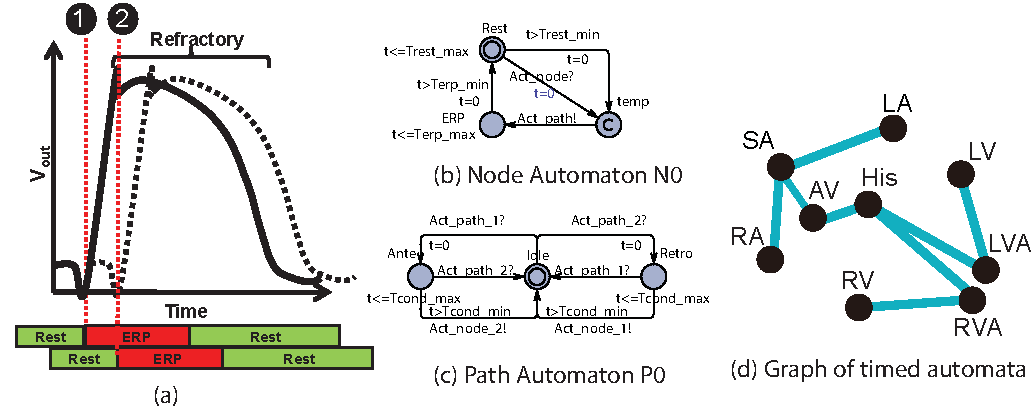
\includegraphics[width=0.9\textwidth]{figs/init_abs.pdf}
	\caption{\small Node and Path Automata which models the timing properties of the heart tissue. A network of node and path automata models the generation and conduction of electrical activities of a heart}
	\label{fig:nodepathTA}
\end{figure}
\subsubsection{Initial Set of Heart Models}
The heart model structure discussed in Chapter 3 is implemented in UPPAAL as shown in \figref{nodepathTA}.
Dynamic changes of the ERP periods and conduction delays are abstracted as ranges using \emph{non-determinism} in timed-automata.
This enables the heart model structure to capture behaviors of the heart models with timing variability.
This heart model structure is based on clinical electrophysiology, with state variables and parameters directly corresponding to physiological parameters.
Therefore, domain experts from clinical electrophysiology can construct models of different heart conditions with their domain expertise and literature.

An example set of initial heart models is shown in \figref{init}.
The different topologies of node and path automata represent the mechanism of different heart diseases.
These heart models represent the current knowledge for heart condition variability, thus the set is inherintly incomplete, meaning there is no guarantee for 100\% safety even if a property is satisfied in all of these models.
These models are mostly used for providing physiological contexts for counter-examples returned by the model checker.
Domain experts can always expand the set with knowledge of new heart conditions.
\begin{figure}[!h]
	\centering
	\includegraphics[width=0.8\textwidth]{figs/init.pdf}
	\caption{\small Examples of the initial set of heart models. The models are different in node and path topology and/or timing parameters.}
	\label{fig:init}
\end{figure}
\subsubsection{Interaction With the Pacemaker}
The interactions between the heart and the pacemaker are modeled by using binary event channels. For the atrial lead, we have:
\textsf{$N_A.Act\_path!\rightarrow$Aget!},
and for ventricular lead we have
\textsf{$N_V.Act\_path!\rightarrow$Vget!}.\\
The pacemaker accordingly generates atrial or ventricular pacing actions \textsf{AP!$\rightarrow N_A.Act\_node!$} and \textsf{VP!$\rightarrow N_V.Act\_node!$}.
\subsubsection{Physiological Abstraction Rules}
The initial set of heart models only represents a subset of all possible conditions.
There always exists conditions that beyond our knowledge or that are combinations of known conditions.
By using \emph{over-approximation}, heart models can be created that cover the observable behaviors of the initial set and that introduce behaviors that were not captured in the initial set.
Inevitably, some of the introduced behaviors will be physiologically invalid.
This problem can be alleviated by carefully designing the abstraction rules so that behaviors introduced are mostly physiologically valid.
The physiologically invalid behaviors can be eliminated during a validity check in the abstraction tree.

Physiological abstraction rules are developed to cover observable behaviors of heart models.
Applying one abstraction rule to heart model(s) $H_1,H_i\dots H_n, n\geq 1$ yields an abstract heart model $H'$ such that all observable behaviors of $H_i$ are covered by $H'$.
For each heart model $H_i$, $H'$ is a \emph{timed simulation} of $H_i$.
To illustrate, a subset of abstraction rules is described intuitively.
The complete set of abstraction rules and the proofs of timed simulation relationship can be found in the tech report \cite{regar_tech}.
%Domain-specific abstraction rules are developed that can introduce new behaviors to a given heart model or a set of models. 
%These new behaviors are physiologically meaningful and might be manifested by a heart condition not explicitly modeled in the initial set of models.
%The physician (or domain expert) remains the ultimate arbiter of what is physiologically meaningful.
%This is a peculiarity of environment modeling, borne out of the fact that the initial set of models is necessarily incomplete, and does not represent all valid behaviors.

%\begin{figure*}[!t]
	%\centering
	%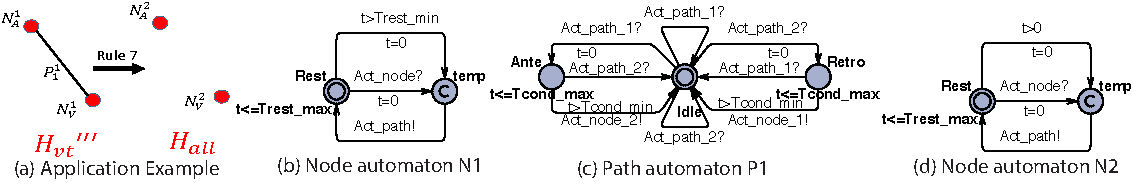
\includegraphics[width=1.05\textwidth]{figs/rule5.pdf}
	%%\vspace{-5pt}
	%\caption{\small (a) Rule 7 application example; (b)(c) Node and path automata used in $H_{vt}'''$; (d) Node automata used in $H_{all}$ }
	%\vspace{-15pt}
	%\label{fig:rule5}
%\end{figure*}
\subsubsection{Rule R1: Convert Reentry Circuits to Activation Nodes}
Within the conduction network of the heart, there can be multiple pathways between two locations, forming conduction loops. If the timing parameters of the tissue along the loop satisfy certain properties, there can be scenarios in which a depolarization wave circling along the circuit. 
The circuits are referred to as \emph{Reentry Circuits}. 
Since the time interval for an activation wave to circle a reentry circuit is usually less than the intrinsic heart cycle length, the heart rate will be "`hijacked"' by the reentry circuit once the cycling is triggered, causing tachycardia. 
Reentry is the most common mechanism for tachycardia, which can be captured by our heart models that are used in \cite{vhm_embc10}. 

The effect of reentry tachycardia is that activation signals coming out of the circuit with a given cycle length equal the sum of conduction delays along the circuit.
It is therefore reasonable to model a reentry circuit as a self-activation node with the self-activation range equal to the sum of conduction delays. \\
\textbf{Applicable Condition: } The rule only affects the topology of the model, and therefore can be applied without preliminaries.\\
\textbf{Output model: }The "essential structure" of a heart model is the shortest paths (in terms of conduction delay) connecting self-activation nodes and/or sensing nodes. 
First detect all circles in the input graph. For each circle with nodes $N_i,i\in[1\dots n]$ and paths $P_j,j\in[1\dots m]$, remove all "non-essential" nodes and paths, create a node automaton $N_s$ and connect to the nearest sensing node with a path automaton $P_s$.\\
\textbf{Effect on parameters: }For the new node automaton $N_s$, the minimum of the Trest parameter is set to the minimum of the sum of the conduction delays within the reentry circuit, and the maximum is set to infinity\\
\textbf{Effect on behaviors: }The new model captures the behavior of the original model when the reentry circuit is active and inactive. Additionally, the new model captures the behaviors of other heart conditions in which the rate of the reentry circuit is lower.
%we have :
%$$N_s.TERP\_min=min(N_i.TERP\_min), N_s.TERP\_max=max(N_i.TERP\_max)$$
%$$N_s.Trest\_min=\sum P_j.Tcond\_min,N_s.Trest\_max=\sum P_j.Tcond\_max$$
%For the new path automaton $P_s$, assume the shortest path from $N_s$ to the nearest sensing node has paths $P_k,k\in[1\dots p]$, we have:
%$$P_s.Tcond\_min=\sum P_k.Tcond\_min,P_s.Tcond\_max=\sum P_k.Tcond\_max$$

\figref{rule1} shows an example in which a circle is replaced by a self-activation node.
\begin{figure}[!h]
	\centering
	\includegraphics[width=0.4\textwidth]{figs/rule1.pdf}
	\caption{\small Rule 1: Remove reentry circuits from the model}
	\label{fig:rule1}
\end{figure}
\subsubsection{Rule R2: Remove Non-essential Structures}
After the circles within the topology are removed, the topology of the heart model is in the form of a tree. Since the "non-essential" structures do not affect the activation signals from and/or to the sensing nodes, all the "non-essential" structures can be removed.\\
\textbf{Applicable Conditions: }The rule can only be applied after Rule 1 has been applied.\\
\textbf{Output model: } Trimmed topology with only the essential structure remaining.\\
\textbf{Effects on parameters: } There are no effects on parameters of the node and path automata.\\
\textbf{Effects on behaviors: } Applying this rule does not affect the observable behaviors of the model.

\figref{rule2} shows an example in which non-essential structures are removed.
\begin{figure}[!h]
	\centering
	\includegraphics[width=0.4\textwidth]{figs/rule2.pdf}
	\caption{\small Rule 2: Remove non-essential structures}
	\label{fig:rule2}
\end{figure}
\subsubsection{Rule 3: Removing Unnecessary Non-self-activation Nodes}
The effect of non-self-activation nodes is blocking electrical events with interval shorter than its ERP period. If the self-activation nodes at both ends of a core path have self-activation interval longer than the maximum ERP period of nodes along the core path, the nodes can be removed.

For a core path from a self-activation node $N_1$ to another core node $N_2$, for any structure $P_1-N_n-P_2$ which $N_n$ is a non-self-activation node, if $N_n.ERP_{max}<min(N_1.Rest_{min},N_2.Rest_{min})$, replace $P_1-N_n-P_2$ with $P_3$ so that:
$$P_3.cond_{min}=P_1.cond_{min}+P_2.cond_{min}$$
$$P_3.cond_{max}=P_1.cond_{max}+P_2.cond_{max}$$

\subsubsection{Rule R4: Merge Parameter Ranges}
Timing periods of heart tissue, such as Rest and ERP, are modeled as locations in the node and path automata. 
The minimum and maximum time an automaton can remain in a location is governed by the parameters in the guards and invariants. 
By merging and expanding these periods, new behaviors are introduced where a heart model may remain longer in Rest, activate or self-activate a node faster, andsoforth.
\\
\textbf{Applicable Conditions: }
This rule applies to heart models with the same node and path topology but possibly with different parameters.\\
\textbf{Output Model: }The abstract model has the same topology as the original models.\\
\textbf{Effects on parameters:} The parameter ranges in the new model are a super-set of the parameter ranges in the old models.\\
\textbf{Effects on behaviors: }The abstract model captures all behaviors of the original models. In addition, heart conditions with parameters outside of the ranges of the original models are covered.
\begin{figure}[!h]
	\centering
	\includegraphics[width=0.7\textwidth]{figs/rule4.pdf}
	\caption{\small Rule 4: Merging parameter ranges}
	\label{fig:rule4}
\end{figure}
\subsubsection{Rule 5: Merge Self-activation Nodes with Interaction Nodes}
%\todo[inline]{not clear}
The effect of self-activation nodes on the interaction of the pacemaker is triggering sensing events within certain delay. In this rule we merge all the self-activation nodes to their neariest interaction nodes. If there exists multiple self-activation nodes merging to the same interaction node, the parameters of the new model are determined following Rule 3.

\subsubsection{Rule R6: Replace Blocking With Non-deterministic Conduction}
%\todo[inline]{in modeling section mention self-activating and passive nodes}
%If a node automaton is in its \textsf{ERP} state, a \textsf{Act\_node} event is "blocked" and will not trigger corresponding path conduction. If we add non-deterministic transitions to the path automata such that a \textsf{Act\_path} event do not trigger state transitions to \textsf{ante} or \textsf{retro} (\figref{rule5}), the blocking behavior of the node is covered. We can then merge the \textsf{ERP} state with the \text{Rest} state in the node automata, and all passive nodes can be removed. An application of Rule 6 is shown in \figref{abs_exam}.\\
Consider the structure $N_1 P_1 N_2 P_2 N_3$ with three nodes and two paths, where $N_2$ is a passive node (i.e. not self-activating).
If $N_2$ blocks an activation signal from $N_1$ to $N_3$, this is equivalent to the paths $P_1$ or $P_2$ not conducting.
In this rule, the structure $P_1 N_2 P_2$ is replaced by a path $P$ whose automaton can take a self loop when it receives an activation signal, thus effectively stopping the conduction. 
This is shown in Fig.~\ref{fig:rule5}: the extra transitions are marked Act\_path\_1? and Act\_path\_2?.
Because the blocking effect of nodes is now incorporated into the paths, the node automata of self-activating nodes can be modified to the one shown in Fig.~\ref{fig:rule5}, which doesn't have the (now useless) ERP period.
\\
\textbf{Subgraph to which it applies}.
Line graphs with 3 vertices $N_1 P_1 N_2 P_2 N_3$, and self-activating nodes.\\
\textbf{Applicability conditions}.
$N_2$ is a passive node.\\
\textbf{Output subgraph}.
$N'_1 P' N'_3$
A path $P'$ whose path automaton is as shown in Fig.~\ref{fig:rule5}.b.
The self-activating nodes $N$ are replaced by nodes $N'$ with automata shown in Fig.~\ref{fig:rule5}.a.\\
\textbf{Effect on parameters}
For the new path, $P.cond_{min}=P_1.cond_{min}+P_2.cond_{min}$ and 
$P.cond_{max}=P_1.cond_{max}+P_2.cond_{max}$
For the new nodes, $N'.Trest_{min}=N.Terp_{min}+N.Trest_{min}$ and 
$N'.Trest_{max}=N.Terp_{max}+N.Trest_{max}$.\\


\begin{figure}[!t]
	\centering
	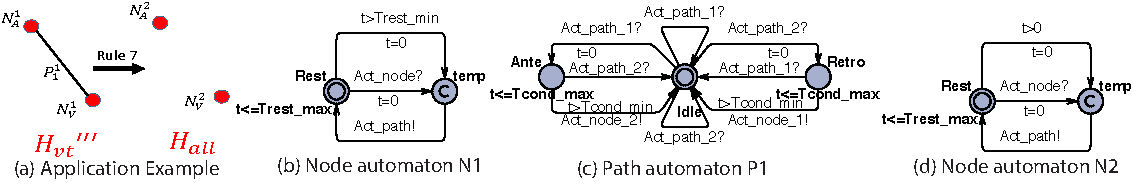
\includegraphics[width=1.05\textwidth]{figs/rule5.pdf}
	%\vspace{-5pt}
	\caption{\small (a) Rule 7 application example; (b)(c) Node and path automata used in $H_{vt}'''$; (d) Node automata used in $H_{all}$ }
	\label{fig:rule5}
\end{figure}

\subsubsection{Rule R7: Replace Conduction With Self-activation}
We describe Rule R7 as it illustrates both effects of an abstraction rule: structure change and modifications to the automata.
The effect of a conduction path is to conduct electrical activity from a node. Since the pacemaker cannot distinguish self-activation of the node and activation triggered by path conduction, we can use self-activation to replace path conduction.
If all self-activation nodes are allowed at any time by setting their minimum Rest period to 0, all the conduction paths can be removed, while preserving the original behaviors (where the Rest period was constrained to a finite interval).\\
\textbf{Applicability conditions}.
This rule can only be applied after Rule 5 and Rule 6 have been applied.\\
\textbf{Output graph}.
All edges are deleted: $G' = (V(G), \emptyset)$. The node automata are replaced with the one shown in \figref{rule5}.d.\\
\textbf{Effect on parameters}
For every node automaton $N$ in $G'$, $N.Trest_{min}=0$.\\

Now we use R7 as example to demonstrate the timed-simulation relationship between heart models before and after the application of R7.
Consider \figref{rule5}.(a) showing an application of R7, $H_{vt}'''=N^1_AP^1N^1_V$ is abstracted to $H_{all}=N^2_AN^2_V$. Here we prove that $H_{vt}'''\preceq_t H_{all}$ with observable events $\Sigma_o=\{N_A.Act\_path,N_V.act\_path\}$. The state of $H_{vt}'''$ is represented by $(N^1_A.loc,P^1_1.loc,N^1_V.loc,N^1_A.t,P^1_1.t,N^1_V.t)$ and the state of $H_{all}$ is represented by $(N^2_A.loc,N^2_V.loc,N^2_A.t,N^2_V.t)$. Due to space limit, only one transition from each category is presented:\\
\textbf{Initial state: }First for the initial state we have:
$$\left\langle (Rest,Idle,Rest,0,0,0),(Rest,Rest,0,0)\right\rangle\in sim_o$$ 
\textbf{Timed transitions: }Consider a timed transition in $H_{vt}'''$
$$(Rest,Idle,Rest,t_1,t_2,t_3)\xrightarrow[]{\tau}(Rest,Idle,Rest,t_1+\tau,t_2+\tau,t_3+\tau)$$
in which $(\tau\in\mathbb{R})\wedge (t_1+\tau\leq N^1_A.Trest\_max)\wedge( t_3+\tau\leq N^1_V.Trest\_max)$. For a state in $H_{all}$ such that $\left\langle (Rest,Idle,Rest,t_1,t_2,t_3),(Rest,Rest,t_1,t_3)\right\rangle\in sim_o$,  there is a timed transition:
$$(Rest,Rest,t_1,t_3)\xrightarrow[]{\tau}(Rest,Rest,t_1+\tau,t_3+\tau)$$
and $\left\langle (Rest,Idle,Rest,t_1+\tau,t_2+\tau,t_3+\tau),(Rest,Rest,t_1+\tau,t_3+\tau)\right\rangle\in sim_o$.\\
%The state of $H_{vt}'''$ is given by the locations of the three automata.
%$$(Rest,Idle,Rest,[Trest\_min, Trest\_max]$$
%$$(Rest,Idle,Rest)\xrightarrow[]{N^1_A.t<N^1_A.Trest\_min \wedge N^1_V.t<N^1_V.Trest\_min}(Rest,Idle,Rest)$$
%are mapped to the following transition in $H_{all}$:
%$$(Rest,Rest)\xrightarrow[]{N^2_A.t<N^2_A.Trest\_min \wedge N^2_V.t<N^2_V.Trest\_min}(Rest,Rest)$$
%
%Self-activations of the atrial node:
%$$(Rest,Idle,Rest,t_1,t_2,t_3)\xrightarrow[\textcolor{red}{N^1_A.Act\_path!}]{t_1\in [N^1_A.Trest\_min, N^1_A.Trest\_max] }(Rest,Ante,0,0,t_3)$$
%are mapped to the following transition in $H_{all}$:
%$$(Rest,Rest,t_1,t_3)\xrightarrow[\textcolor{red}{N^2_A.Act\_path!}]{t_1\in [0, N^2_A.Trest\_max]}(Rest,Rest,0,t_3)$$
%Self-activations of the ventricular node:
%$$(Rest,Idle,Rest,t_1,t_2,t_3)\xrightarrow[\textcolor{red}{N^1_V.Act\_path!}]{t_3\in [N^1_V.Trest\_min, N^1_V.Trest\_max] }(Rest,Retro,Rest,t_1,0,0)$$
%are mapped to the following transition in $H_{all}$:
%$$(Rest,Rest,t_1,t_3)\xrightarrow[\textcolor{red}{N^2_V.Act\_path!}]{t_3\in [0, N^2_V.Trest\_max]}(Rest,Rest,t_1,0)$$
\textbf{Discrete transitions: }Consider a discrete transition in $H_{vt}'''$
$$(Rest,Ante,Rest,t_1,t_2,t_3)\xrightarrow[t_2\in [P^1_1.Tcond\_min, P^1_1.Tcond\_max) ]{\textcolor{red}{N^1_V.Act\_path!}}(Rest,Idle,Rest,t_1,t_2,0)$$
in which $N^1_V.Act\_path!\in\Sigma_o$. \\
For a state in $H_{all}$ such that $\left\langle (Rest,Idle,Rest,t_1,t_2,t_3) ,(Rest,Rest,t_1,t_3)\right\rangle\in sim_o$,  there is a discrete transition:
$$(Rest,Rest,t_1,t_3)\xrightarrow[t_3\in [0, N^2_V.Trest\_max)]{\textcolor{red}{N^2_V.Act\_path!}}(Rest,Rest,t_1,0)$$
and $\left\langle ((Rest,Idle,Rest,t_1,t_2,0)),(Rest,Rest,t_1,0)\right\rangle\in sim_o$. Basically activation due to conduction is replaced by self-activation of the corresponding node automata.\\
\textbf{Additional behaviors: }The timed-simulation also allows additional behaviors into $H_{all}$. Consider a discrete transition in $H_{all}$
$$(Rest,Rest,t_1,t_3)\xrightarrow[t_3\in [0, N^2_V.Trest\_min)]{\textcolor{red}{N^2_V.Act\_path!}}(Rest,Rest,t_1,0)$$
However, for a state in $H_{vt}'''$ such that $\left\langle (Rest,Idle,Rest,t_1,t_2,t_3),(Rest,Rest,t_1,t_3)\right\rangle\in sim_o$, when $t_3\in [0, N^1_V.Trest\_min]$ there is no available discrete transitions. Physiologically, these implicitly included behaviors correspond to fast heart rate, premature heart events and even noise.



\subsubsection{Abstraction Tree}
By applying the abstraction rules to the initial set of heart models, an abstraction tree is created.
\figref{HM_abs} shows an example of an abstraction tree with the root model capturing all possible input sequences to the pacemaker.
Self-activating nodes are marked as red and the Trest parameters are specified next to them.
Note that this abstraction tree is not unique.
With a different initial set of heart models and/or different rule application orders the abstraction tree can be very different.
The abstraction tree can also be extended at any time if new heart conditions are specified.
The following section demonstrates the use of this abstraction tree during the closed-loop model checking of the pacemaker design.

 \begin{figure*}[!t]
	\centering
	\includegraphics[width=0.95\textwidth]{figs/abs_tree.pdf}
	%\vspace{-5pt}
	\caption{\small One example of abstraction tree of heart models}
	\label{fig:HM_abs}
\end{figure*}


\section{Efficacy Validation for Implantable Pacemaker}
The most essential function for the pacemaker is to treat bradycardia by maintaining the ventricular rate above a certain threshold. We define the region where the ventricular rate is slow, as \textsf{unsafe}. The monitor \textsf{PLRI\_test} is designed to measure intervals between ventricular events and is shown in \figref{safety1}. For property
\begin{center}
\textsf{$\varphi_{LRI}=$A[] (PLRI\_test.secV imply PLRI\_test.t$\leq$TLRI)}
\end{center}
we have a closed-loop system with heart model $H_0$ : 
$$H_0\| P\| PLRI\_test\models\varphi_{LRI}$$

\begin{figure*}[b]
\centering
%\vspace{-10pt}
		\subfigure[Monitor \textsf{PLRI\_test}] {
				\includegraphics[width=0.4\textwidth]{figs/LRI_test.pdf}
				\label{fig:safety1}
		} 
		\subfigure[Monitor \textsf{PURI\_test}] {	
			\includegraphics[width=0.3\textwidth]{figs/uri_test.pdf}
			\label{fig:uri_test}
		}
		%\vspace{-10pt}
	\caption{(a) Monitor for LRL: Interval between two ventricular events should be less than TLRI, (b) Monitor for URL: Interval between a ventricular event and a VP should be longer than TURI}
\end{figure*} 

The pacemaker is not designed to treat tachycardia so it can only pace the heart to increase its rate and cannot slow it down. To mitigate the hazard that the pacemaker may increase the heart rate above physiological need, an Upper Rate Interval (URI) is specified such that the pacemaker can increase the ventricular rate up to this limit. 
  
We require that a ventricle pace (VP) can only occur at least $TURI$ after a ventricle event (VS, VP). The monitor \textsf{PURI\_test} is shown in \figref{uri_test}. For the property
\begin{center}
$\varphi_{URI}=$\textsf{A[] (PURI\_test.secV imply PURI\_test.t$\geq$TURI)}
\end{center}
we have: $$H_0\| P\| PURI\_test\models \varphi_{URI}$$

As we saw in the above examples, the efficacy requirements are satisfied with the most abstract heart model.
Therefore no heart model refinements are necessary and the requirements are satisfied under all possible heart conditions.

%\section{Evaluate the Mitigation}
%As described in Chapter \ref{Mode_switch}, the mode switch algorithm has been designed to mitigate the hazard that the A-V synchrony function of DDD pacemaker extends fast
%atrial rate to the ventricle. It is important to ensure the effectiveness of the algorithm without inducing other top-level hazards. In this section we first show the existence of the hazard in a pacemaker without the mode-switch algorithm. If the algorithm if effective the hazard will not exist after introducing the algorithm.
%
%\subsection{Existence of Pacemaker Mediated Tachycardia during SVT}
%The monitor \textsf{Pv\_v} is designed to show existence of PMT during SVT. It goes to the error state if the ventricular rate drops below the Upper Rate Limit (\figref{vv}).  
%
%
%We specify 
%$\varphi_{MS}=E[] (not Pv\_v.err)$\\
%which verifies the existence of PMT. The heart model $H_e$ in Fig. \ref{fig:HM_abs} is not suitable for this property since the non-deterministic conduction of component $P_3$ does not capture the blocking property of the AV node, which is the key in PMT. We use a more refined model $H_d$ which has AV node modeled. To identify the PMT scenario, we first set $H_d.N^1.Trest\_min<100$ so that the atrial rate can be high and $H_d.N^2.Trest\_min>TURI$ so that the intrinsic heart rate is less than TURI. The property is first verified on pacemaker without the mode-switch algorithm. We have $H_d\|P\|Pv\_v\models\varphi_{MS}$ and the evidence returned by the model checker illustrates the PMT scenario.
%
%% There are two separate AVI and LRI components for each mode and switches to the corresponding ones when synchronization signals are received. The clock values are kept so that essential intervals are kept. 
%\subsection{Verification against fundamental safety properties}
%For a pacemaker with the mode switch algorithm: 
%
%$P_2$=\textsf{LRI'$\|$AVI'$\|$URI$\|$PVARP$\|$VRP$\|$INT$\|$CNT$\|$DUR}, 
%
%we verify the same fundamental safety properties on the pacemaker model with mode-switch algorithm. We have:
%$$H_d\|P_2\|PURI\_test\models\varphi_{URI}$$
%$$H_d\|P_2\|PLRI\_test\not\models\varphi_{LRI}$$


\section{Safety Validation for Implantable Pacemaker}
A dual chamber pacemaker is designed to increase the heart rate during bradycardia, but it should also not increase the heart rate inappropriately.
Inappropriate increase of heart rate by the pacemaker is referred to as \emph{Pacemaker Mediated Tachycardia (PMT)}.
Previous work \cite{STTT13} used model checking to identify two known PMT conditions.
However, in order to avoid ambiguities in the counter-examples, the properties for the two PMTs were specified very specifically, which abandoned the advantage of model checking to find unknown safety violations.

With the abstraction tree approach, the ambiguities can potentially be resolved since the abstraction tree considers all known heart conditions.
Therefore the property for PMTs can be specified more generally.
In this paper, we specify a property such that\\
$\varphi_{PMT}$: \emph{The interval between ventricular events (Vget, VP) should not be shorter than TURI for 30 consecutive beats}\\
which means that the ventricular rate should not be faster than the upper rate interval (TURI) for too long, either intrinsically or because of pacemaker interaction.
Counter-example because of intrinsic fast ventricular rates can be removed from results after analysis from the abstraction tree.

A UPPAAL monitor $M_{con}$ for the property is shown in Fig. \ref{fig:monitor}, and the TCTL property is specified as:\\
\begin{center}
\emph{A[] not $M_{con}$.err}
\end{center}

\begin{figure}[!t]
	\centering
	\includegraphics[width=0.4\textwidth]{figs/monitor.png}
	\caption{\small UPPAAL monitor for Property 1}
	\label{fig:monitor}
\end{figure}

The model checker UPPAAL was used to check Property $\varphi_{PMT}$ on the pacemaker model using the abstraction tree of heart models.
The property is violated in $H0 || PM$, thus thus the abstraction tree is followed to select pair $H1$ with the pacemaker model and Property 1 is verified again.
The process continues till either the leaves of the tree are reached of the property is satisfied.
The result is shown in \figref{CE}, which demonstrates 5 different scenarios that can happen when using the abstraction tree.
The shaded area marks the heart models with counter-examples.
\begin{figure*}[!t]
	\centering
	\includegraphics[width=0.8\textwidth]{figs/tree.pdf}
	%\vspace{-5pt}
	\caption{\small Four different physiological conditions in which Property 1 is violated. In $CE_{af}$ the pacemaker extends a fast atrial rate to a dangerously fast ventricular rate; in $CE_{vt}$ the ventricular rate is intrinsically fast; in $CE_{st}$ the pacemaker appropriately maintained A-V conduction delay; in $CE_{pvc}$ the pacemaker inappropriately increased the ventricular rate, causing Endless Loop Tachycardia}
	\label{fig:CE}
\end{figure*}

\textbf{Case 1:} Property 1 is violated in $H2\_1 || PM$ but is satisfied in its children $H3\_1 || PM$.
Careful examination of the counterexample finds it to be spurious and so it is successfully eliminated by model refinement.

\textbf{Case 2:} $CE_{af}$ is returned by $H3\_2 || PM$ and corresponds to intrinsic atrial tachycardia with fast atrial rate, which is a sub-optimal but non-lethal condition.
The AV node of the heart will block a subset of the electrical events and maintain a normal ventricular rate.
However, despite the filters in the pacemaker, the pacemaker still paces the ventricle for every 3 atrial activations, which extends fast atrial rate to more dangerous fast ventricular rate. 
The condition is referred to as Atrial Tachycardia Response in which the ventricular rate is increased inappropriately, thus requires revision of the pacemaker design.

\textbf{Case 3:} $CE_{vt}$ is returned by $H3\_3 || PM$ and corresponds to intrinsic ventricular tachycardia with fast ventricular rate.
The counter-example is physiologically valid but the fast ventricular rate is due to the heart itself and is beyond pacemaker functionality.
Therefore this scenario demands no revision of the pacemaker design.

\textbf{Case 4:}  $CE_{st}$ is returned by $H3\_5 || PM$ and corresponds to sinus tachycardia, for instance, when the patient is exercising.
The pacemaker improved the open-loop heart condition by pacing the ventricles $AVI$ after each atrial event, which is a correct operation of the pacemaker despite the requirement violation. 

\textbf{Case 5:} $CE_{pvc}$ is returned by $H4\_4 || PM$ and has a very similar input-output relationship to $CE_{n}$. 
However, the activations of the atrial node are triggered by retrograde conduction from ventricular paces (marker \textsf{cond}). 
The atrial activations trigger another ventricular pace after $AVI$, which will trigger another retrograde conduction. In this case the heart rate is inappropriately high, which corresponds to a dangerous closed-loop behavior referred to as \emph{Endless Loop Tachycardia}.

From the above result, it can be seen that abstraction tree is able to 1) refine a heart model to eliminate spurious counter-examples as in Case 1; 2) provide (multiple) physiological explanations to a counter-example as in Case 2-5; and 3) resolve ambiguities caused by abstraction as in Case 4 and 5.

Device manufacturers have developed algorithms aiming to eliminate behaviors showed in Case 2 and Case 5.
In the following section we demonstrate the use of abstraction tree to evaluate the effectiveness of these algorithms.

\subsection{Terminating Endless Loop Tachycardia}


%\begin{figure*}
		%\centering
		%%\vspace{-20pt}
		%\includegraphics[width=0.7\textwidth]{figs/pelt_det.pdf}
		%%\vspace{-15pt}
		%\caption{\small (a) Any pattern other than VP-AS will result in error state (b) If the ventricular rate is slower than the Upper Rate Limit will go to error state}
		 %% \vspace{-15pt}
		%\label{fig:elt_det}
%\end{figure*}

Due to the limited information the pacemaker has about the heart, the pacemaker cannot distinguish a retrograde atrial event from an intrinsic atrial event which is triggered by the SA node. From the pacemaker's point of view, the pacemaker paces the ventricles as specified for every AS. That is why open-loop testing is unable to detect this closed-loop behavior. 

Modern pacemakers are equipped with anti-ELT algorithms to identify and terminate potential ELT. One common algorithm identifies ELT by the ELT pattern and terminates ELT by increasing TPVARP time once to block the AS caused by the V-A conduction. By increasing the blocking interval after a ventricular event, the pacemaker effectively ignores the early atrial signal detected due to the PVC.
\begin{figure*}
		\centering
		%\vspace{-10pt}
		\includegraphics[width=0.7\textwidth]{figs/ELT_count.pdf}
		%\vspace{-20pt}
		\caption{\small (1) The component \textsf{PVAS} sends \textsf{VP\_AS!} event when a VP-AS pattern with delay between [150,200] is detected; (2) Component \textsf{ELTct}. After 8 VP-AS pattern, the algorithm increase TPVARP to 500ms. (3) Modified \textsf{PVARP'} component. TPVARP can only be set to 500 for one timing cycle.}
		 % \vspace{-15pt}
		\label{fig:ELT_count}
\end{figure*}
%\subsection{Existence of ELT}
%Two monitors were designed to show the existence of ELT. One monitor, \textsf{PELT\_det}, shows the persistence of the VP-AS pattern and the other monitor, \textsf{Pvv}, shows that the ventricular rate is always no slower than the upper rate limit (\figref{elt_det}). The property \\
%\textsf{$\varphi_{ELT}=$E[] ((not PELT\_det.err) $\&\&$ (not Pvv.err))}\\
%checks the existence of ELT behavior. After our initial verification we have:\\
%$H_4\|P\|PELT\_det\|Pvv\models\varphi_{ELT}$
%
%The evidence trace shows the behavior of the system. For simplicity we only show the state of the heart:\\
%$RE\|RE\xrightarrow[VP!\rightarrow Act\_node\_2!]{AVI.t\geq TAVI \wedge URI.t\geq TURI}$\\
%$RE\|RE\xrightarrow[Act\_path\_1!\rightarrow AS!]{N^1.t\geq 0}$\\
%$RE\|RE\xrightarrow[VP!\rightarrow Act\_node\_2!]{AVI.t\geq TAVI \wedge URI.t\geq TURI}$\\
%$RE\|RE\xrightarrow[Act\_path\_1!\rightarrow AS!]{N^1.t\geq 0}$\\
%$RE\|RE$
%
%\subsection{Trace Validation and Heart Model Refinement}
%We check this trace on more refined $H_3\| P$ and discovered that the trace above can correspond to two different scenarios:\\
%$RE\|AN\|RE\xrightarrow[VP!\rightarrow Act\_node\_2!]{AVI.t\geq TAVI \wedge URI.t\geq TURI}$\\
%$RE\|ID\|RE\xrightarrow[Act\_path\_1!\rightarrow AS!]{N^1.t\geq N^1.Trest\_min}$\\
%$RE\|AN\|RE\xrightarrow[VP!\rightarrow Act\_node\_2!]{AVI.t\geq TAVI \wedge URI.t\geq TURI}$\\
%$RE\|ID\|RE\xrightarrow[Act\_path\_1!\rightarrow AS!]{N^1.t\geq N^1.Trest\_min}$
%$RE\|AN\|RE$\\
%and\\
%$RE\|ID\|RE\xrightarrow[VP!\rightarrow Act\_node\_2!]{AVI.t\geq TAVI \wedge URI.t\geq TURI}$\\
%$RE\|RT\|RE\xrightarrow[Act\_node\_1!\rightarrow Act\_path\_1!\rightarrow AS!]{P.t\geq P.Tcond\_min}$\\
%$RE\|ID\|RE\xrightarrow[VP!\rightarrow Act\_node\_2!]{AVI.t\geq TAVI \wedge URI.t\geq TURI}$\\
%$RE\|RT\|RE\xrightarrow[Act\_node\_1!\rightarrow Act\_path\_1!\rightarrow AS!]{P.t\geq P.Tcond\_min}$\\
%$RE\|ID\|RE$
%
%Both traces correspond to actual clinical scenarios. However, the second trace corresponds to the ELT behavior which inappropriately increased the heart rate. By setting $N^1.Trest\_min\geq TURI$ in $H_3$ we can model the healthy heart and the first scenario will be eliminated. However, in $H_4$ the $Trest\_min$ is set to 0 so the two cases cannot be distinguished. So we use the refined heart model $H_3$ with $N^1.Trest\_min\geq TURI$.
%With the new heart model we have:\\
%$H_3\|P\|PELT\_det\|Pvv\models\varphi_{ELT}$\\
%The evidence trace, which is exactly the second trace above, shows exactly the ELT scenario.
%%\subsection{Heart Model Refinement 1}
%The property failed because the RHM cannot distinguish an intrinsic atrial event and a retrograde atrial event and we cannot set their parameters separately to represent a more complex heart condition. In order to deal with this problem, we refine our RHM by adding a non-deterministic A-V conduction \textsf{Cond\_n} (\figref{cond}) between the atrial channel and the ventricular channel. Events from \textsf{RHM\_A} can trigger ventricular event \textsf{V\_act!} with delay, which mimics the intrinsic A-V conduction. Ventricular events can trigger retrograde conduction to the atria, causing event \textsf{A\_retro!}. Since the intrinsic ventricular events are modeled by \textsf{Cond\_n}, \textsf{RHM\_V} is replaced with a PVC component (\figref{PXC}). The refined heart model \textsf{Refinement 1} is shown in \figref{refine}.
%\begin{figure}
%		\centering
%		%\vspace{-15pt}
%		\includegraphics[width=0.45\textwidth]{figs/cond.pdf}
%%		%\vspace{-20pt}
%		\caption{\small \textsf{Aget!} event can either trigger \textsf{V\_act!} event after delay or do nothing. \textsf{PVC!} event can either trigger \textsf{A\_retro!} event after delay or do nothing}
%		 %\vspace{-15pt}
%		\label{fig:cond}
%\end{figure}
%
%Since $\mathbb{T}(PVC)=\mathbb{R}$, we have $\mathbb{T}(PVC)\bigcup\mathbb{T}(V\_act)=\mathbb{R}$. We also have $\mathbb{T}(A\_retro)=\mathbb{T}(PVC)\bigcup\mathbb{T}(V\_act)$+ $[Tretromin, Tretromax]=\mathbb{R}$ and $\mathbb{T}(A\_retro)\bigcup\mathbb{T}(Aget)=\mathbb{R}$ thus the refinement is proper abstraction of the VHM. With the refined heart model we can adjust $\mathbb{T}(Aget)$ without changing $\mathbb{T}(A\_retro)$. The existence property holds and the evidence returned by UPPAAL shows an ELT execution trace.
%\begin{figure*}
%\centering
%%\vspace{-10pt}
		%\subfigure []{
				%\includegraphics[width=0.4\textwidth]{figs/SVT_none.pdf}
				%\label{fig:SVT_none}
		%} 
		%\subfigure []{	
			%\includegraphics[width=0.4\textwidth]{figs/SVT_DDD.pdf}
			%\label{fig:SVT_DDD}
		%}
		%%\vspace{-10pt}
	%\caption{(a) Open-loop: 3:1 A-V conduction during SVT and low ventricular rate without SVT; (b) With DDD pacemaker: the pacemaker paces the ventricle for every atrial sense (AS), thus increase the ventricular rate inappropriately}
%\vspace{-10pt}
%\end{figure*} 
\subsubsection{ELT termination algorithm} 
The ELT persists without intervention and the patient's heart is forced to beat at a fast rate approaching the Upper Rate Limit. Thus, device manufacturers require a way to identify ELT and terminate it despite the limited information the pacemaker can get. The ELT detection algorithm by Boston Scientific \cite{challenge} utilizes these three features:
\begin{itemize}
  \item Ventricular rate at Upper Rate Limit
	\item VP-AS pattern
	\item Fixed V-A conduction delay
\end{itemize}
The pacemaker first monitors VP-AS pattern with ventricular rate at upper rate limit. Then it compares the VP-AS interval with previous intervals. ELT is confirmed if the difference between the current VP-AS interval and the first VP-AS interval is within $\pm$32ms for 8 consecutive times. Then the pacemaker increases the PVARP period to 500ms once so that the next AS will be blocked and will not trigger a VP, terminating ELT.
As the V-A conduction delays are patient-specific, the algorithm compares the VP-AS interval to a previously sensed value instead of an absolute value. Since we can not store past clock values in UPPAAL, we can not explicitly model this ELT detection algorithm. However, since the conduction delay in our heart model is within a known range, we can compare the VP-AS interval with this range. The VP-AS pattern detection module $VPAS$ for our anti-ELT algorithm is shown in \figref{ELT_count} (1). It detects the VP-AS pattern with ventricular rate at the Upper Rate Limit and sends out a \emph{VP\_AS} event if the interval qualifies. 

A counter $ELTct$ counts the number of qualified VP-AS patterns. It increases the PVARP period to 500ms if eight consecutive VP-AS patterns are detected. (\figref{ELT_count} (2)) The PVARP component is also modified so that the PVARP period can only be changed once by the anti-ELT algorithm. (\figref{ELT_count} (3))

\subsubsection{Verification of the algorithm}
With the new pacemaker model\\ 
$P_1=LRI\|AVI\|URI\|PVARP'\|VRP\|ELTct\|VPAS$\\
we first check whether the two efficacy properties still hold when the anti-ELT algorithm is introduced. We have 
$$H_0\|P_1\|PLRI\_test\models\varphi_{LRI}$$
$$H_0\|P_1\|PURI\_test\models\varphi_{URI}$$
Indicating the efficacy properties still hold after introducing the anti-ELT algorithm.

Then property $\varphi_{PMT}$ is checked, we have
$$H2\_4\|P_1\|PELT\_det\|Pvv\not\models\varphi_{PMT}$$
which indicates the algorithm successfully eliminated all ELT executions.

\subsection{Mode Switch Operation: Atrial Tachycardia Response}
\label{Mode_switch}

Pacemaker manufacturers have designed algorithms to detect and terminate behaviors as in $CE_{af}$. Intuitively, the mode-switch algorithm first detects SVT. After confirmed detection, it switches the pacemaker from a dual-chamber mode to a single-chamber mode. During the single-chamber mode, the A-V synchrony function of the pacemaker is deactivated thus the ventricular rate is decoupled from the fast atrial rate. After the algorithm determines the end of SVT, it will switch the pacemaker back to the dual chamber mode. 
\begin{figure*}
		\centering
		%\vspace{-19pt}
		\includegraphics[width=0.8\textwidth]{figs/AVI_ms.pdf}
		%\vspace{-10pt}
		\caption{\small (a) After switching to \textsf{VDI} mode, the new LRI component \textsf{LRI'} maintains a minimum V-V interval; (b) After switching to \textsf{VDI} mode, the new AVI component \textsf{AVI'} keeps track of the time after each atrial events.}
		%  \vspace{-20pt}
		\label{fig:avi_ms}
\end{figure*}
The mode-switch algorithm (also known as atrial tachycardia response) specification we use is similar to the one described in the Boston Scientific pacemakers' manual (\cite{compass}). The algorithm first measures the interval between atrial events outside the blanking period (AS, AR). The interval is considered as \emph{fast} if it is above a threshold (\emph{Trigger Rate}) and \emph{slow} otherwise. In our UPPAAL model we model it as $INT$ (see \figref{dur_count} (1)). A counter $CNT$ increments for \emph{fast} events and decrements for \emph{slow} events (see \figref{dur_count} (2)). After the counter value reaches the \emph{Entry Count}, the algorithm will start a \emph{Duration} ($DUR$) ,which is a time interval used to confirm the detection of SVT (see \figref{dur_count} (3)). In the \emph{Duration}, the counter keeps counting. If the counter value is still positive after the \emph{Duration}, the pacemaker will switch to the VDI mode (\emph{Fallback mode}). In the VDI mode, the pacemaker only senses and paces the ventricle. At any time if the counter reaches zero, the \emph{Duration} will terminate and the pacemaker is switched back to DDD mode.
% to show some interesting findings. The basic idea of this simplified model is explained in detail. \\
%\mySubSubSection{UPPAAL model for mode-switch algorithm}
In our UPPAAL model of the mode-switch algorithm, we use nominal parameter values from the clinical setting. We define \emph{trigger rate} at 170bpm (350ms), \emph{entry count} at 8, \emph{duration} for 8 ventricular events and \emph{fallback mode} as VDI. 
\begin{figure*}
		\centering
				%\vspace{-15pt}
		\includegraphics[width=0.9\textwidth]{figs/duration.pdf}
		%\vspace{-10pt}
		\caption{\small (1) Component \textsf{INT}: An atrial event (\textsf{AS,AR}) arrives before \textsf{thresh} after the previous atrial event is regarded as a \textsf{fast} event. Atrial event arrives after \textsf{thresh} and \textsf{AP} are regarded as \textsf{slow} event; (2) Component \textsf{CNT}: After 8 \textsf{fast} event the algorithm will start a duration by sending \textsf{du\_beg} and will switch to \textsf{VDI} mode when the duration ends (\textsf{du\_end}); (3) Component \textsf{DUR} :The duration length is 8 ventricular events (\textsf{VS,VP})}
		  %\vspace{-15pt}
		\label{fig:dur_count}
\end{figure*} 

In order to model both DDD and VDI modes and the switching between them, we made modifications to the AVI and LRI components.
In each component two copies for both modes are modeled, and switch between each other when switching events (DDD, VDI) are received. During VDI mode, \textsf{VP} is delivered by the LRI component instead of the AVI component. The clock values are shared between both copies in order to preserve essential intervals even after switching. The modified AVI ($AVI'$) and LRI ($LRI'$)components are shown in \figref{avi_ms}. 

\subsubsection{Verification of the Mode-Switch Algorithm}
With the new pacemaker model\\ 
$P_2=LRI'\|AVI'\|URI\|PVARP'\|VRP\|INT\|CNT\|DUR$\\
we first check whether the two efficacy properties still hold when the anti-ELT algorithm is introduced. We have 
$$H_0\|P_2\|PLRI\_test\not\models\varphi_{LRI}$$
$$H_0\|P_2\|PURI\_test\models\varphi_{URI}$$
By analyzing the counter-example we found that when the pacemaker is switching from VDI mode to DDD mode, the responsibility to deliver VP switched from LRI component to AVI component. Since the clock reference is different (Ventricular events in LRI component and Atrial events in AVI component), the clock value for delivering the next VP is not preserved. As a result, if an atrial event which triggered the mode-switch from VDI to DDD happens within [TLRI-TAVI, TLRI) after the last ventricular event, the next ventricular pacing will be delayed by at most TAVI time, which violates the Lower Rate Limit property (\figref{safety}). 
%%\begin{figure}
%%		\centering
%%		\includegraphics[width=0.4\textwidth]{figs/vv.pdf}
%%		\caption{\small Monitor \textsf{Pv\_v} for SVT: There exists an endless sequence in which interval between ventricular events is at most TURI}
%%		  %\vspace{-15pt}
%%		\label{fig:vv}
%%\end{figure}
Then property $\varphi_{PMT}$ is checked, we have
$$H3\_2\|P_1\|PELT\_det\|Pvv\not\models\varphi_{PMT}$$
Indicating the mode-switch algorithm failed to eliminate the PMT scenario. The counter-example trace returned by UPPAAL shows that a subset of atrial events fall into the blanking period after a ventricular event (see \figref{liveness}). As a result, two fast events are reduced to one slow event and mode switch may never happen. Therefore the mode-switch algorithm in our pacemaker model can not terminate all PMT behaviors as specified as certain mild PMT events are admissible.
\begin{figure}
\centering
%\vspace{-20pt}
		\subfigure []{
				\includegraphics[width=0.4\textwidth]{figs/safety.pdf}
				\label{fig:safety}
		} 
		\subfigure []{	
			\includegraphics[width=0.4\textwidth]{figs/liveness.pdf}
			\label{fig:liveness}
		}
	\caption{(a) Safety Violation: VP is delayed due to the reset of timer during mode-switch, (b) Efficacy Violation: The blocking period may block some atrial events, turning two \emph{Fast} events to one \emph{Slow} event (\cite{TACAS12}})
\end{figure} 

\section{Discussion}
Model checking is not widely use in industry, in part, due to scalability issues and also because domain expertise must be a skill possessed by the verification engineer. 
However, with rigorous abstraction of the system and its environment, model checking can be used to identify 
known and even unknown mechanisms to induce hazards. 
In this chapter, we used a model of a dual chamber pacemaker as an example to demonstrate the use of model checking during risk analysis. 
During the process we identified the need to refine the heart models to eliminate false-positives introduced during the abstraction, and demonstrated the difficulty to do so manually. 
The abstraction tree approach is then proposed to reduce the effort needed for both the developers and the domain experts, which makes model checking a viable approach for providing safety and effectiveness evidence. 
With the abstraction tree of heart models, safety and efficacy violations are identified within the pacemaker specification, which demonstrates the capability of model checking to identify issues during the early development of autonomous medical devices.

\chapter{Theme 3: Verified Model to Verified Code}
Model checking is performed on abstract models of the system, which is at an early stage in the development process. The verified system model during model checking is then translated into a Stateflow model, which is a step towards simulation-based testing and subsequently to code generation. Closed-loop simulation/testing are performed on more refined deterministic models, and on the actual system, complement model checking in terms of resolving ambiguities within abstract counterexamples. We aim to answer the following questions here:

\begin{itemize}
	\vspace{-5pt}
	\item How are abstract models translated to deterministic models for simulation-based testing?
	\vspace{-5pt}
	\item What system level issues are best tested at the platform level?
\end{itemize}

In this chapter, we first describe an approach to automatically translate formal models that are verified in UPPAAL to Stateflow charts for simulation-based testing, and then code generated to run on an embedded platform. Following this, we demonstrate two examples that cannot be explicitly modeled using abstract semantics and must be tested.

\section{UPPAAL to Stateflow Automated Model Translation}
%%%%%%%%%%%%%%%%%%%%%%%%%%%%%%%%%%%%%%%%%%%%
\begin{figure*}[!b]
\centering
		\subfigure 
		{			
		\includegraphics[width=0.45\textwidth]{figs/method_new1.png}		
		\label{fig:method}
		}
		\hspace{.2in} 
		\subfigure 
		{	
			\includegraphics[width=0.45\textwidth]{figs/chart_GlobalClocks_rev1.png}
			\label{fig:chart}
		}
\caption{(a)~Model Driven Design framework: From UPPAAL to Stateflow to generated code -- covering model verification, simulation-based testing and platform testing.~(b) Structure of Stateflow charts of the pacemaker's five basic timing cycles (from Fig. \ref{fig:PMdesign}) derived by the UPP2SF model translator. Parent states $P_1,...,P_n$ are derived from automata, while the \textit{clock} states $Gc\_{x_1},..., Gc\_{x_m}$ model all global clocks $x_1,...,x_m$ from the UPPAAL model. The state $Eng$ is used to control execution of the chart.}
\label{fig:upp2sftool}
\end{figure*} 
%%%%%%%%%%%%%%%%%%%%%%%%%%%%%%%%%%%%%%%%%%%%

A model translation tool, UPP2SF (\cite{TECS}) was developed to translate UPPAAL models to Stateflow (see \figref{method}). Consider an UPPAAL model with automata $P_1,...,P_n$.  After UPP2SF translation, a two-level Stateflow chart is generated as in \figref{chart}. The chart consists of parallel states $P_1,...,P_n$ (referred to as the \textit{parent} states) derived from the automata, parallel states $Gc\_{x_1},..., Gc\_{x_m}$ (referred to as \textit{clock states}) that model all global clocks $x_1,...,x_m$ from the UPPAAL model, and the state $Eng$ that is used as the chart's control execution engine.
Moreover, the chart has predefined global data variables (and constants) with appropriate ranges and initial values derived from the UPPAAL model. 
Since all automata in UPPAAL are active simultaneously, the obtained Stateflow chart is a collection of parallel states with unique execution orders. Also, in every UPPAAL automaton exactly one location is active at a time. Thus, each of the parent states is a collection of exclusive states, extracted from locations in the corresponding UPPAAL automaton. 

In \cite{TECS}, we showed that for a large class of UPPAAL models, the generated Stateflow models generated by UPP2SF preserve behaviors of the initial UPPAAL models. The translation tool can be used to estimate the worst case execution time (WCET) during modeling and model checking stage in UPPAAL, and facilitates development of modular code from timed-automata based models. 

%%\begin{figure} [!t]
%%\center
%%\includegraphics[width=0.48\textwidth]{figs/chart_GlobalClocks_rev1.png} 
%%\caption{}
%%\label{fig:chart}
%%\end{figure}

\figref{PM_sf} demonstrates the Stateflow chart generated from the UPPAAL model of the DDD pacemaker model in \figref{PMdesign} using the UPP2SF tool.
\begin{figure*} [!t]
\center
\includegraphics[width=0.77\textwidth]{figs/PM_SF_buffer_newC1.png} 
\caption{Pacemaker Stateflow chart converted from the UPPAAL model in~\figref{PMdesign} using UPP2SF; the heart and buffer models are highlighted.} 
\label{fig:PM_sf}
\end{figure*}
We generated C code from the pacemaker Stateflow chart using the Simulink Coder. The code structure is shown in \figref{pm_code}.
The code was generated for the general embedded real-time target and as a result we obtained the main procedure, \texttt{rt\_OneStep}, which processes the three input events, $VinB$, $AinB$ and $clk$. To ensure that the model semantics are preserved (modulo the execution time), $clk$ input events should be created every 1ms, followed by the procedure's activation. This makes it suitable for implementation on top of a real-time operating system (RTOS).

\begin{figure*} [!t]
\center
\includegraphics[width=\textwidth]{figs/CodeListingFinal.png}
\caption{Structure of the pacemaker code obtained from the Stateflow chart shown in \figref{PM_sf}.}
\label{fig:pm_code}
\end{figure*}


The pacemaker code generated by the Simulink Real-Time Workshop's Embedded Coder was executed on nanoRK (\cite{nanork}), a fixed-priority preemptive RTOS that runs on a variety of resource constrained platforms. We tested the implementation on the TI MSP-EXP430F5438 Experimenter Board interfaced with a signal generator that provides inputs for the pacemaker code (\figref{setup}). More details regarding UPP2SF translation and platform testing can be found in \cite{TECS}.

%%%%%%%%%%%%%%%%%%%%%%%%%%%%%%%%%%%%%%%%%%%%
\begin{figure*}[!t]
\centering
		\subfigure 
		{			
		\includegraphics[width=0.46\textwidth]{figs/HM_PM_newMon.png}
		\label{fig:hm_pm}
		}
		\subfigure 
		{	
			\includegraphics[width=0.48\textwidth]{figs/HW_setup1.png}
			\label{fig:PM_timer}
		} 
\caption{(a)~Structure of the pacemaker model in UPPAAL and Stateflow, including the interaction between the pacemaker and heart, and the monitors used for verification. (b) Hardware setup with MSP430F5438 experimenters board.}
\label{fig:setup}
\end{figure*} 
%%%%%%%%%%%%%%%%%%%%%%%%%%%%%%%%%%%%%%%%%%%%



\subsection{Summary:}
In this chapter, we first introduced a model translation method from UPPAAL timed automata models to Stateflow charts. Combined with Simulink coder, the tool chain provides rigorous evidence of traceability from physiological requirements to the C code implementation. Oversensing, crosstalk and lead displacement are three examples in which the cause of the problem is not modeled in the abstract interface in the timed-automata model. In such cases, closed-loop testing with the more refined heart models and EGM interface can be used to provide safety evidence.


%\subsection{Acknowledgements}
%\begin{acknowledgements}
%\addcontentsline{toc}{chapter}{Acknowledgements} 
%The authors would like to thank Houssam Abbas, Rajeev Alur, George M. Chen, Allison Connolly, Sanjay Dixit, Insup Lee, Pieter Mosterman, Miroslav Pajic, Oleg Sokolsky and Larisa G. Tereshchenko for fruitful discussions during the preparation of this manuscript. This research was supported in part by NSF CNS-0720518, NSF CNS-1035715, NSF MRI-0923518, NSF CPS Frontier 1446664 and NSF CAREER-1253842 grants. This work was also supported in part by STARnet - a Semiconductor Research Corporation program sponsored by MARCO and DARPA.
%\end{acknowledgements}
%%\chapter{Certification}
%%\begin{itemize}
%%          	\item What is the current practice for medical device certification? What are the limitations?
%%          	\item Can model-based closed-loop verification provide more safety guarantee to complement current practice? By how much?
%%          \end{itemize}
%%          
%%\section{Current Practice}
%%%In United States, medical devices have to be approved by FDA to be released into the market. 
%%According to their potential risks the devices are categorized into 3 classes, Class I, Class II and Class III, corresponding to low-risk, medium-risk and high-risk devices \cite{class}. Life-sustaining devices like implantable pacemakers are classified as Class III and in general are subject to the most strict regulations.
%%
%%There are two processes that a medical device can enter the market in U.S.: the Premarket Notification, also known as 510(k) \cite{510k}, and the Pre-Market Approval (PMA) \cite{PMA}. In a 510(k) submission the device manufacturers are only required to provide evidence that the device is \emph{substantial equivalent} to a \emph{predicate device}, which has been approved for the market. Therefore, the 510(k) submission does not directly require clinical evidence for the safety and effectiveness of the device, thus is suitable for mostly low-risk devices like Class I and Class II devices.  The Pre-Market Approval (PMA) submission is a more stringent regulatory process in which direct clinical evidence is required to prove the safety and effectiveness of the device. However, not all Class III devices are subject to PMA submission. If a Class III device clears the 510(k) process and FDA has not requested PMA for that device, the device is still cleared for market release. A study shows that for Class III devices which PMA has been requested, the levels of evidence varies. Only 40\% of the PMA submissions are supported by controlled clinical trials, which provide the most rigorous clinical evidence \cite{cert_prob}. The lack of quality evidence is usually due to the high cost of the controlled clinical trials.
%%\section{Evidence from Model-based Design}
%%%\cite{pancreas}
%%Model-based verification provides a low-cost solution to provide reasonable evidence for the safety and effectiveness of the devices. The open questions are:
%%
%%\begin{itemize}
%%	\item How valid are the models?
%%	\item How much confidence can they provide?
%%\end{itemize}

\chapter{Theme 4: in-silico Pre-clinical Trials for Implantable Cardiac Devices} 
\section{Clinical trials and RIGHT}
\label{sec:rcts}

At the clinical trial stage (Fig.~\ref{fig:spectrum}), the objective is no longer to find bugs in the device: it is, rather, to evaluate the safety and efficacy of the validated device on humans. 
RCT are the gold standard for evaluating the safety and efficacy of a new medical device \cite{FriedmanFD10_ClinicalTrials}.
They constitute the only time prior to market use where the effects of the device on humans are actually observed, and are legally mandated for new high-risk medical devices like ICD.
%It is important to understand how a typical RCT proceeds to appreciate where CPS modeling can help in that process.
%Very broadly, in an \ac{RCT}, a new treatment also known as the \emph{intervention}, is compared to the current standard of care, commonly known as the \emph{control}.
%For example, two competing ICDs are compared.
%Each patient recruited to the trial is randomly assigned to either the intervention or the control group and undergoes the corresponding treatment.
%At the end of the trial, any clinically relevant differences between the two groups are evaluated to determine if they are statistically significant.
The planning and execution of an RCT requires carefully navigating a number of technical, logistical and ethical issues to obtain reliable and statistically significant results.

Because of the very high cost of RCT in terms of money, time, and the risk of harm they present to enrolled patients, our focus in this paper is on the use of CPS models, formalized in an MBCT, \emph{to validate the assumptions made by the investigators and thus increase the chances of success of an RCT}.
We illustrate our approach by applying it to the Rhythm ID Going Head-to-Head Trial (RIGHT) \cite{GoldABBTB11_RIGHTresults}, which we present next.

\subsection{The RIGHT trial}
\label{sec:right}
We first provide a brief background to better understand RIGHT (see Fig.\ref{fig:icd}). Tachycardias (abnormally elevated heart rates) can be divided into VT, which originate in the heart's ventricles, 
and SVT, which originate above the ventricles.
A sustained VT can be fatal, while an SVT is typically non-fatal.
The therapy applied by the ICD often takes the form of a high-energy electric shock.
The shock can be pro-arrhythmic, and was even linked to increased morbidity \cite{shock_mortality}.
Therefore, one of the biggest challenges for ICDs is to guarantee shock delivery for VT, and simultaneously reduce inappropriate shocks during SVT \cite{Ellenbogen11_Pacingbook}.

RIGHT is a trial that sought to compare the VT/SVT discrimination abilities of two algorithms \cite{GoldABBTB11_RIGHTresults}: 
the Rhythm ID detection algorithm found in Boston Scientific's Vitality II ICDs~\cite{compass},
and the PR Logic + Wavelet (PRL+W) detection algorithm found in a number of Medtronic's ICDs (Medtronic Maximo,
Marquis, Intrinsic, Virtuoso, or Entrust ICD).
%\mynote{SD}{make sure to list all the Boston Scientific and Medtronics ICD models that use each of these algorithims. This is very important}
%The investigators chose the following primary question: is there a difference in time-to-first inappropriate therapy between the two ICDs?
\emph{Inappropriate therapy} was defined as therapy applied to an arrhythmia other than VT or VF (VF is a type of VT).
RIGHT enrolled 1962 patients and ran for approximately five years.
It was fully sponsored by Boston Scientific. 

One of the trial's assumptions was that Rhythm ID would reduce the risk of inappropriate therapy by 25\% over PRL+W~\cite{Berger06_RIGHT}.
The outcome of the trial~\cite{GoldABBTB11_RIGHTresults}, however, was that patients implanted with ICDs running Rhythm ID had a \emph{\textbf{34\% risk increase}} of inappropriate therapy as compared to patients implanted with ICD running PRL+W. 
This result  is the opposite of the effect hypothesized by the trial investigators. 
In this paper, we design an MBCT to test early and quickly whether the hypothesized effect holds by comparing the two ICDs on a large \emph{synthetic} cohort.\\\\
\textbf{\emph{Organization:}} In the following sections we describe the building blocks of the MBCT: modeling the heart, processing 100's of real patients' data, mapping the timing and morphology components of the signal to a heart model we developed, generating a population of 10,000+ synthetic heart models, implementing the device algorithms and conducting multiple trials for the comparative rate of inappropriate therapy, condition-level rates and evaluating the effect of device parameters on discrimination rates.

 \section{Heart Modeling}
 \label{sec:heart modeling}
%The first step in any MBCT is to choose a patient model that can interact with the device in a closed loop. 
%Computer models of the heart have been developed to model different aspects of the cardiac function to suit different applications (\cite{natalia,Grosu_wave}).
%In this section we first give a brief overview of the basic Electrophysiology of the heart which describes the electrical activation and conduction, which is the basis for ICDs. 
%We also describe our effort to model the electrical activity of the heart to generate signals corresponding to a large range of heart conditions that the ICD can encounter.

\subsection{Basic cardiac electrophysiology}
\label{sec:cardiac ep}
The heart has two upper chambers called the \emph{atria} and two lower chambers called the \emph{ventricles} (see Fig. \ref{fig:icd})
The synchronized contractions of atria and ventricles assure an adequate supply of oxygenated blood to the rest of the body.
This contraction is driven by electrical activity in the heart.
A normal pattern of electrical activity is referred to as NSR.
Disturbances of NSR are referred to as \emph{arrhythmias}, and can result in insufficient blood supply and even death of a patient. 
\emph{VT} is an example of an arrhythmia originating in the ventricles, in which the ventricles beat at a very high rate.
If the VT is sustained, or degenerates into VF, it is fatal within seconds.
An abnormally fast heart rate that originates in the atria and/or the conductinon system above the ventricles is referred to as a \emph{SVT}.
This is not a fatal condition but does cause patient discomfort and its treatment is elective.
Many arrhythmias fall under this heading.

Implantable Cardioverter Defibrillators (ICDs) can diagnose VT and VF by observing the electrical activity through three channels, as shown in Fig.~\ref{fig:icd}.
The measured signals are known as \emph{electrograms}, or EGMs.
VT and SVT can share similar heart rates and might even occur simultaneously, so an SVT can be mis-diagnosed as a VT. 
This is problematic because VT therapy consists of low and high energy electric shocks of 30-40 Joules ($\sim$800V) delivered directly to the heart, which is very painful to the patient, and has been shown to increase morbidity \cite{shock_mortality}\footnote{\small{Physicians compare a shock to a ``horse kicking you in the chest"}}.
Therefore, one of the biggest challenges for ICDs is to discriminate between VT that typically requires a shock, and SVT that typically should not be shocked \cite{Ellenbogen11_Pacingbook}.

An EGM signal can be characterized by the \emph{timing of events} that produced it, and the \emph{morphology of the signal itself}.
An `event' is roughly characterized as the source of the largest peak in the EGM (e.g. a ventricular depolarization), and event timing is a crucial element of an arrhythmia's definition in clinical Electrophysiology.
The `morphology' refers to the shape of the EGM (see Fig. \ref{fig:adjudication} for examples).
Both aspects are used by the ICD to make its decision.
Correspondingly, our model has two components: a timing model, and a morphology model.

\subsection{Timing Model}
\begin{figure}[t]
	\centering
	\vspace{-10pt}
	\includegraphics[width=0.3\textwidth]{figs/HM_top.pdf}
	\caption{\small Timing model of the heart}
	\vspace{-10pt}
	\label{fig:HM_top}
\end{figure}
Computer models of the heart have been developed to model different aspects of the cardiac function to suit different applications (\cite{natalia}).
In \cite{VHM_proc}, the authors developed a heart model structure that can be used to simulate the timing for generation and conduction of electrical events of the heart under a variety of conditions.
The model structure consists of a set of node automata, which model the \emph{generation} and \emph{blocking} of electrical events by heart tissue, and a set of path automata, which model the \emph{conduction delay} of electrical activity between node automata.
The node and path topology used in the MBCT is shown in Fig. \ref{fig:HM_top}. 
The hollow nodes are passive nodes representing key locations within the heart where electrical events may be blocked. These include the Atrioventricular node (AV), Right Bundle Branch (RBB) and Left Ventricle Apex (LVA). 
The filled nodes in red, Sinoatrial (SA) node and Right Ventricle Apex (RVA) node, represent the heart locations where ICD electrodes are placed to measure the EGMs.
The timing of the activation events at these nodes determines the timing of corresponding EGMs.
Different sources for tachyarrhythmias are represented by arrhythmia nodes (dashed filled nodes) which are capable of self-activating at prescribed rates. These include Premature Atrial Complexes (PACs) and Premature Ventricular Complexes (PVCs) which are sources of rhythm disturbances.

Every node and path automaton has timing parameters that determine, for example, the delay between events, and how long it takes to conduct an electrical event between two nodes.
These timing parameters can be directly derived from clinical data \cite{josephson}, and the model structure is compatible with clinical Electrophysiology concepts.
Thus we know the ranges for these parameters.
In \cite{VHM_proc}, the timing model's capability to simulate various normal and abnormal heart conditions was validated quantitatively and by cardiac electrophysiologists.


In this work we use the same heart model structure to ensure the correct timing of the EGM signals into the ICD.
%The nodes in orange are capable of self-activation at different rate determined by corresponding parameters, which represent different sources for tachy-arrhythmia.
%Since in this study we do not need the heart models to react to device therapy.
In order to account for inherent timing variability, during simulation the heart model randomly selects timing parameters within a pre-specified range, instead of choosing specific values. 
By choosing the range, we control the variability of the signals produced by a given model instance.

\subsection{Morphology Model}
The ICD uses the EGM morphology in two ways:
first, the atrial and ventricular EGMs are used to \emph{sense} when events occur via peak detection (Section \ref{sec:sensing}).
Second, the Shock channel EGM is used in the morphology comparison discriminators (Section \ref{sec:svtvt}, \cite{VTC,Wavelet}).
It is known that sensing (the detection of events) can be responsible for up to 20\% of inappropriate therapies \cite{wrong_sensing}.
Therefore, it is important that our model generate realistic and varied EGM waveforms for a proper evaluation of the detection algorithms.

\begin{figure}[t]
	\centering
%	\vspace{-5pt}
	\includegraphics[scale=0.3]{figures/figEGMGeneration1column.pdf}
	\vspace{-15pt}
	\caption{\small EGM waveform generation.
		From a given model instance and set of tachycardias, an EGM waveform is generated for the duration of an episode. The timing model determines event timings. When an event occurs, the EGM morphology for the event is output from the morphology model.  
		}
	\vspace{-15pt}
	\label{fig:egmGeneration}
\end{figure}
The timing model provides the time stamps for electrical events to happen at the interfacing nodes (SA,RVA). 
From path conduction we also know the source of the signals.
In the heart model structure shown in Fig. \ref{fig:HM_top} there are 5 different sources for SA node activation and 5 different sources for RVA node activation. 
Based on the clinical observations that electrical events from the same source produce very similar EGM morphologies, we can generate EGM signals by overlaying EGM templates corresponding to different sources onto the timing event diagram.
The procedure is shown in Fig. \ref{fig:egmGeneration}.
We also introduce small variations on EGM templates.
The variations are obtained by a wavelet decomposition of the signatures followed by a random scaling of the 25\% smallest coefficients.
We guarantee that this does not change the signature of the EGM, by running one of the morphology comparison discriminators described in Section \ref{sec:svtvt}.
This variation is parametrized, e.g. the percentage of modified coefficients, the range of the random scaling.

\subsection{Patient Data Adjudication and EGM Template Extraction}
In order to obtain realistic morphologies for our simulations we utilize the Ann Arbor Electrogram Libraries (AAEL), a database of over 500 EGM recordings made during clinical electrophysiology studies~\cite{AAEL}. 
The AAEL is used by all major ICD manufacturers and is licensed by the US FDA. 
The AAEL provides descriptive annotations of records at a high level.
We performed additional detailed examination to precisely segment each record according to rhythm type.
123 records from 47 patients were manually examined and adjudicated into segments called \emph{episodes} containing one specific rhythm, e.g. NSR or VF. 
The adjudication was performed by a cardiologist.
Fig. \ref{fig:adjudication} (left) shows an example record (Record A185660) which has undergone this adjudication.
%It should be noted that only with a standard 12-lead \ac{ECG} in addition to ICD signals can all types of arrhythmia be accurately diagnosed.
From each episode, we developed an automated process which extracted EGMs from a given episode. 
The EGM are collected and organized by both patient record and by the type of rhythm which was annotated during the adjudication process.
These extracted rhythm \emph{signatures} provide the basis for the morphology information in the signal generated by our model.
Fig. \ref{fig:adjudication} (right) depicts an example of 10 signatures extracted from the record. 

\begin{figure*}[t]
	\centering
	\vspace{-10pt}
	\includegraphics[scale=0.35]{figures/figadjudication.pdf}
	\vspace{-10pt}
	\caption{\small  (Left) The EGM record is segmented into episodes with distinct rhythms in each. (Right) From each episode, individual EGM morphologies are extracted and stored.
	}
	\label{fig:adjudication}
\end{figure*}

\subsection{Cohort generation}
\label{sec:cohort generation}
Let $p = (p_1,\ldots,p_n) \in \Re^n$ be the vector of timing and morphological parameters of the heart model.
Let $P_i \subset \Re$ be the range of parameter $p_i$.
We generate a \emph{synthetic cohort} of $N$ probabilistic model instances.
To produce one of these instances, for each scalar parameter $p_i$, we randomly select a sub-interval $I_i$ of its range: $I_i \subset P_i$.
The sub-interval $I_i$ is chosen so that it fits with the tachycardia that this model instance is meant to simulate.
E.g., for modeling VT, the rest period of the VT node might be assigned the sub-interval $I_i = [260, 280]ms$, reflecting the firing rate in the ventricles.
%Two different instances of the same tachycardia will, in general, have different sub-intervals within $P_i$.
When a model instance is simulated, each parameter $p_i$'s value changes beat to beat by sampling it uniformly within its sub-interval $I_i$.
Thus each generated model is probabilistic to reflect inherent rhythm variability.

\section{Implementing Device Algorithms} 
\label{sec:device models}
Due to the limited sensing capability of ICDs, device manufacturers have developed different algorithms to identify the electrical events and correctly diagnose the cardiac arrhythmia as being VT or SVT.
In this paper we implemented the detection algorithm Rhythm ID of Boston Scientific \cite{compass,Ellenbogen11_Pacingbook},% [???Compass, pacingdefibrillation,VTC paper, ICD book, Ellenbogen].
and PRLogic+Wavelet (PRL+W) of Medtronic \cite{Singer,Wavelet}.
%In available literature on the evaluations of device algorithms descriptions of the device algorithms are not detailed enough for full implementation.
%To obtain the detailed implementation we further reviewed clinical execution traces from literature like \cite{Singer} to infer detailed executions of the algorithms. 
We also set up a testing platform to validate our implementations against real ICDs using conformance testing.
\subsection{Cardiac Signal Sensing}
\label{sec:sensing}

%Basic definition and principle
\emph{Sensing} is the process by which cardiac signals measured through the leads of the ICD is converted to cardiac timing events.
Appropriate sensing is essential for proper ICD detection algorithm operation which relies heavily on accurate event timing and morphology information provided by sensing. 
An \emph{event} corresponds to a depolarization in the heart and manifests as a displacement from the baseline amplitude of the signal.
In its simplest form, the sensing algorithm declares an event whenever the amplitude of the signal exceeds a given threshold.
Once an event has been declared, the peak of the amplitude is measured and a \emph{refractory period} begins, during which a consecutive event is ignored for a short period of time. 
This is to ensure that the same event is not counted repeatedly.

%Difficulty of sensing
ICDs require a balance in sensitivity in order to operate in noisy, complex, environments where cardiac events can vary greatly in signal amplitude and frequency, such as during VF. 
Setting the threshold low achieves higher sensitivity to events of small amplitude, but increases the chances for incorrectly sensing other cardiac electrical artifacts such as T-waves and noise artifacts (oversensing). 
Conversely, setting the threshold too high allows sensing to be more robust to noise and other cardiac electrical events, but creates the potential for undersensing events of interest, such as during VF when the peak amplitude can be low. 

%Enhancement 1: 
In order to achieve adequate balance, ICD sensing algorithms are enhanced by applying dynamic adjustment of the sensitivity threshold.
Initially, the threshold is raised during the refractory period after an event and once the refractory period concludes, the threshold is decayed to a minimum pre-set threshold.
In our device models, we implemented the AGC algorithm of Boston Scientific and the AAS of Medtronic ICDs to incorporate dynamic threshold adjustment. 

%%Enhancement 2: Cross-chamber blanking
%In addition to \ac{AGC}, in our device model for Boston Scientific, we have implemented a specific \emph{cross-chamber blanking} feature present in Boston Scientific \ac{ICD}s. 
%Cross-chamber blanking starts a blanking period in atrial sensing after a ventricular event has been detected.
%This reduces the chance of a ventricular event being interpreted as an atrial event.

The complexity of these enhancements adds to the difficulty of properly programming device settings of ICDs and requires calibration process at the time of ICD implantation and during patient follow-up visits.
\subsection{VT Detection Algorithm}
\label{sec:svtvt}
%The limited sensing resolution and noise in the \ac{EGM} signals make it is impossible for the device to achieve 100\% accuracy for SVT/VT discrimination.
Device companies have developed different algorithmic components to distinguish SVT from VT, referred to as \emph{discriminators}. 
Each discriminator utilizes the history of timing and/or morphology of the EGM signals to determine whether the current rhythm is a VT or SVT (or neither).
%The decisions of each discriminators are then combined using a decision tree structure to decide whether to deliver or inhibit therapy.
No single discriminator is sufficient on its own to discriminate between SVT and VT, because these classes of arrhythmias can appear similar in a number of criteria.
Therefore discriminators are organized in a decision tree.%, as illustrated in Fig. \ref{fig:BS_det}.
We have implemented the detection algorithms Rhythm ID from Boston Scientific and PRL+W from Medtronic. 
This section gives an overview of both algorithms.

%We will need the following definition: an \emph{interval} is the amount of time between two consecutive electrical events. 
%Thus a ventricular interval is the duration between two ventricular events.
%Intervals are variable in length. 
%Consistently short intervals imply a fast rhythm.

\begin{figure*}[t]
	\centering
	\includegraphics[scale=0.38]{figs/BS_det.pdf}
	\vspace{-10pt}
	\caption{\small SVT/VT detection algorithm by Boston Scientific \cite{compass}. The two cases on the right illustrate two different decisions by the algorithm. (a) illustrates a sustained VT case where at the end of the Duration, the ventricular rate is faster than the atrial rate. The algorithm correctly identified the rhythm as VT and delivered therapy. (b) illustrates a SVT case where at the end of the Duration, the ventricular rate is slower than the atrial rate. Then by comparing the EGM morphology in the Shock channel (Marker 1) with the stored NSR template (Marker 2) for the last 10 EGM events, the algorithm decided that the morphology is correlated, therefore therapy is inhibited.}
	\label{fig:BS_det}
\end{figure*}

\subsubsection{Rhythm ID}
Rhythm ID's decision tree is shown in Fig.~\ref{fig:BS_det}.
Rhythm ID detects an episode by continuously examining the last 10 ventricular intervals and comparing them with VT and VF thresholds. 
If 8/10 intervals are shorter than the VF threshold for a certain pre-set \emph{VF Duration} (e.g., 2.5 seconds) then the algorithm declares VF.
Otherwise, if 8/10 intervals are shorter than the VT threshold for a certain VT Duration, then further discriminators are used.
First, if the ventricular rate is greater than the atrial rate for the last 10 ventricular beats, Rhythm ID will determine the condition is VT.
Otherwise, the Vector Timing and Correlation (VTC) discriminator~\cite{VTC} compares EGM morphology of the last 10 ventricular events with an EGM \emph{template} saved during NSR.
VTC is based on the assumption that the EGM morphology of the shock channel during VT is different from its morphology during SVT and NSR.
If the correlation between the current EGM's morphology and the stored NSR morphology is above a pre-set threshold, the current rhythm is more likely to be SVT than VT, and therapy is withheld.
Otherwise, if the atrial rate is equal to a pre-set fibrillation rate and the variance of the ventricular interval length exceeds a certain limit, the algorithm decides it's an SVT. 
Otherwise, it decides this is a VT.
%As shown in Fig. \ref{fig:BS_det}(b), at the end of the duration, the atrial rate is faster than the ventricular rate. 
%The morphology in the shock channel is similar to the NSR morphology (red dashed) so VTC is correlated and therapy is inhibited.
%As a comparison the morphology during VT is different from the NSR morphology (Marker 1 in Fig. \ref{fig:BS_det}).

\subsubsection{PR Logic+Wavelet}
PRL+W also utilizes rate-based and morphology-based discriminators similar (but not identical) to Rhythm ID.
The morphology discriminator used in PRL+W  is similar to VTC in Rhythm ID, but operates in the wavelet domain~\cite{Wavelet}.
PRL+W also continuously compares the pattern of atrial and ventricular activation to 19 pre-defined patterns~\cite{Singer}.
Each pattern is associated to a heart condition, like Sinus Tachycardia or VT.
A match between the current activity and one of the pre-defined patterns is used as an indication that the current rhythm is explained by the associated condition.

\subsection{Validation}
\label{sec:validation}
%\begin{figure}[t]
%	\centering
%	\includegraphics[scale=0.28]{figures/figValidationSetup.pdf}
%	\vspace{-10pt}
%	\caption{\small Model Validation. 14 different scenarios were generated from the EGM waveform generator for Boston Scientific and input into the Vitality 2 ICD. The input signal was acquired through the DAQ board and applied to the device model implementation. The ICD response was interrogated using the ICD programmer and compared to the output of the device model.}
%	\vspace{-10pt}
%	\label{fig:validationSetup}
%\end{figure}

\begin{figure}[t ]
	\centering
	\includegraphics[scale=0.28]{figures/figScreenshot.pdf}
	\caption{\small Example of validation output screenshots (Ventricular fibrillation) showing matching therapy decision for the ICD and our implementation.}
	\vspace{-10pt}
	\label{fig:validation}
\end{figure}

Conformance testing was used to validate the software implementations of the Vitality II device by Boston Scientific. 
The validation hardware setup is illustrated in Fig.~\ref{fig:validation}. 
14 different scenarios were specified and programmed into an EGM Waveform generator (CRM3 Simulator, Guidant, USA) such that it would output a signal to the connected Vitality II device.
The various scenarios traverse 7 out of 9 branches of the detection algorithm for Boston Scientific described in Sec. \ref{sec:svtvt} and shown in Fig. \ref{fig:BS_det}. 
The response of the ICD interrogated using an ICD programmer (ZOOM Latitiude, Boston Scientific).
As the waveform was applied to the ICD, the waveform was simultaneously acquired using a National Instruments DAQ board.
The recorded waveform was then applied to the device model and response was compared.
Fig. \ref{fig:validation} shows an example of one such scenario, specificallly VF. 
In this case, the software model matched to the decision of the actual ICD which also determined that therapy should be applied.

In all scenarios, the decision of model conformed to that of the ICD. 
The remaining two branches were not reachable due to the limited output capability of the programmer.
The Medtronic software implementation can be validated using a similar process.

\section{Results}

\subsection{The rate of inappropriate therapy}
\label{sec:rate inapp}
%\todo[inline]{justify episode-level rates and not patient-level}
The first objective of the MBCT is to estimate the rate of inappropriate detection $\bar{t}$ for each of the two algorithms for all arrhythmias combined, i.e., for the entire synthetic cohort.
The rate of inappropriate therapy is defined as
\[\bar{t} = \frac{\text{Number of inappropriately applied therapies}}{\text{Number of applied therapies}}\]
From this we can confirm or invalidate the assumption that Rhythm ID outperforms PRL+W.
We generated a synthetic cohort of 11,400 heart instances, equally distributed among the 19 arrhythmias.
The number of instances was obtained from a Monte Carlo calculation.% whose details follow the presentation of the results.

\textbf{Conclusion 1: PRL+W delivers less inappropriate therapy.}
The obtained rates of inappropriate detection were 6.65\% for Boston Scientific and 2.91\% for Medtronic (P < 0.0001), assuming an equal number of patients from each arrhythmia in the synthetic cohort.
The corresponding relative improvement \emph{of Medtronic over Boston Scientific} is 56\%.
In other words, the MBCT reveals that the PRL+W algorithm from Medtronic actually differentiates between VT and SVT better than Rhythm ID from Boston Scientific.
Our findings are consistent with the observations of the RIGHT trial itself~\cite{GoldABBTB11_RIGHTresults}.

\textbf{Conclusion 2: result holds across population characteristics.}
The above rates were obtained under the assumption that each arrhythmia is equally represented in the cohort.
A significant feature of MBCT is that it allows us to study the endpoint of interest (here, rate of inappropriate detection) on a variety of populations, which have the various arrhythmias in different proportions.
This may not be feasible in a real clinical trial, which has to contend with the population present at the clinical centers where the trial is conducted.
We may then ask: does PRL+W maintain a lower rate of inappropriate detection across different populations?
To answer this question, we varied the distribution of the arrhythmias in the synthetic cohort, and re-computed the cohort-wide rates of inappropriate therapy.
Fig. \ref{fig:popvar8} shows the results for 10 random variations of the arrhythmia distribution.
It can be seen that indeed, PRL+W maintains a better rate of arrhythmia discrimination (and by inference, less inappropriate therapy) across the board.
%Thus the results are robust to the characteristics of the population under study.
%\mynote{SD}{Delete last sentence}

\begin{figure*}[t]
	\vspace{-10pt}
\centering
\vspace{-10pt}
\includegraphics[scale=0.4]{figures/popvar9}
\caption{\small Rate of inappropriate detection ($2^{nd}$ and $4^{th}$ columns) for different arrhythmia distributions ($1^{st}$ and $3^d$ columns). The arrhythmias are (left to right on the x axis): Atrial fibrillation, Atrial flutter, Premature Ventricular Complexes, Nonsustained Ventricular Fibrillation, Supraventricular Tachycardia, Sinus Brady-Tachy, Ventricular Fibrillation, Ventricular Tachycardia \cite{josephson}. The top left distribution is uniform, and the bottom right distribution is that of the baseline characterization in RIGHT \cite{GoldABBTB11_RIGHTresults}.}
\label{fig:popvar8}
\end{figure*}

This illustrates very well the benefit that an MBCT can bring to the planning of an RCT: the fact that Rhythm ID could not be shown to be better than PRL+W %(let alone 25\% better as was hypothesized by the investigators) 
can cause the investigators to re-consider their assumptions and the feasibility of the trial.
In this case, the MBCT casts doubt on the assumed \emph{direction} of the effect, i.e. whether intervention is better than control, or the other way around.
This early check can mean the difference between an expensive trial that fails at showing the desired effect, and a trial that is appropriately sized to demonstrate the desired effect size.

%While we will not know the true distribution of the arrhythmias in the \ac{RCT} until its completion, 
Thus, while an MBCT does not replace or mimic the RCT since we can not capture patient-level outcomes of the therapy, it can provide  but \emph{early insight} at a small fraction of the RCT cost and duration and without the ethical issues.	 

%\textbf{Sample size calculation for MBCT}.
%The rate is naturally computed as the mean of a random variable.
%Namely, it is the mean of the variable $t$ which equals 1 if the episode is a VT/VF for which therapy was applied, and 0 if it's a VT/VF for which therapy was withheld.
%To get reliable estimates for this rate, we use a standard Monte-Carlo calculation under the assumption that the estimate of the mean is normally distributed around the true mean. 
%This is justified by the central limit theorem and the fact that we can generate a very large number of hearts for each rhythm.
%By choosing a confidence interval width of 0.001 around the mean, we obtain a sample size of 9,604 hearts.
%In our experiments we used 11,400 to decrease the empirical variance of the estimate.
%The 95\% confidence interval around the mean estimate is given by $CI = \hat{t} \pm z_{95}\frac{S_t}{\sqrt{n}}$, 
%where $\hat{t}$ is the mean estimate, $z_c$ is the $c\%$ confidence level (so $z_{95}=1.96$), 
%$S_t$ is the empirical variance, 
%and $n$ is the number of Monte Carlo simulations, i.e., the number of heart instances we will generate and simulate for a given rhythm.
%The larger the number of simulations $n$, the tighter the confidence interval around the estimate.
%The rates we estimate fall in the range $[0,1]$ and are significant to the second decimal digit.
%Because we are considering all arrhythmias combined, we assume a conservative empirical variance $S_x$ to be 0.05, (validated experimentally) and set the desired confidence interval half-width to 0.001:
%\[\1.96\frac{0.05}{\sqrt{n}} = 0.001\]
%This yields $n = 9604$.
%In the experiments we use $n=11400$ to help guarantee the assumed empirical variance.
%The obtained empirical variance is invariably much smaller than 0.05.

%The obtained results for sensitivity and inappropriate therapy rate are shown 
%\begin{table}[b]
%	\smallcaption{Sensitivity and inappropriate therapy rate.}
%	\begin{tabular}{|p{1.9cm}|c|p{2.5cm}|}
%		\hline             & \textbf{Boston Sci.}(\%)   & \textbf{Medtronic} (\%)\\
%		\hline Sensitivity &  100                   &  100  \\ 
%		\hline Inappropriate therapy rate &  6.65                   &  2.91 \\ 
%		\hline 
%	\end{tabular}
%	\label{table:total nbs}
%\end{table} 

%We may also define a hypothesis test, which we illustrate for the rate of inappropriate therapy.
%The null hypothesis $H_{0,t}$ is that the rates for $\bar{t}$ are equal for Medtronic and Boston Scientific devices.
%\[H_{0,t}: \bar{t}_{MED} = \bar{t}_{BSC}  \]
%The alternative hypotheses are that the rates are not equal.
%In all that follows, `effect size' refers to the relative difference between the two rates.
%
%We assume an effect size of 27\%: this is based on the \emph{episode-level} inappropriate therapy rates reported in RIGHT (Table 2 of \cite{GoldABBTB11_RIGHTresults}).
%(Note that some of those reported results, however, were not statistically significant at the 5\% significance level).
%At the 5\% significance level and 90\% power, this yields a sample size of 11160.
%% with an assumed BSC rate of 0.08.
%We used 11400 instances in our MBCT.
%The results were inappropriate therapy rates $\bar{t}_{BSC}= 0.0291$ and $\bar{t}_{MED} = 0.0665$, with an effect size (relative to Medtronic's algorithm) of 56\% with $P << 10^{-3}$.
%Thus the null hypothesis of equality of inappropriate therapy rates can be rejected.

\subsection{Condition-level rates}
\label{sec:condition-level}
Having a heart model allows us to better estimate the \emph{sensitivity} and \emph{specificity} of the diagnostic algorithms' performance, something which is not possible in a clinical trial because the device only records a limited number of episodes.
These are defined as
\[ \text{Sensitivity} = \frac{\text{Number of correctly classified VTs}}{\text{Number of true VTs}}\]
\[ \text{Specificity} = \frac{\text{Number of correctly classified SVTs}}{\text{Number of true SVTs}}\]
In words, the sensitivity measures how well the device recognizes VTs.
Specificity measures how well the device discriminates between VT and SVT.
An ideal device would have 100\% sensitivity and specificity.
Unfortunately, these are typically competing goals: the more sensitive the device, the more likely it will mis-diagnose some SVTs as VTs, so its specificity will drop.
%During a clinical trial, the implanted ICD is typically set to record only treated episodes, so it is not possible to obtain all episodes and measure specificity.
%Moreover, if a VT episode is non-sustained, it won't receive therapy and won't be recorded, so it's not possible to measure sensitivity.
%Even if the device were set to record all episodes whether treated or not, memory limitations mean that it won't record everything.

We calculated sensitivity and specificity in our MBCT, and report them in Table \ref{table:vtsvt} on a per-arrhythmia basis.
The conditions are drawn from RIGHT's baseline characterization \cite{GoldABBTB11_RIGHTresults}.
Specificity is reported for SVTs and sensitivity is reported for VTs.
It can be seen from these results that in our synthetic cohort, Atrial flutter and other Supraventricular tachycardias are the main source of inappropriate detection for Rhythm ID compared to PRL+W.
In the case of Atrial flutter, Rhythm ID categorizes it inappropriately as VT for 41.7\% of the cases.

Condition-level analysis pinpoints the specific pathways of the discrimination algorithm which must be addressed to reduce the device's rate of inappropriate therapy. It is difficult to get such insight through an RCT as the patient population is fixed and the conditions are determined retroactively. Such analysis can be further used to investigate condition distributions across different patient population types (e.g. abnormal heart rhythms in children vs geographic region-specific or race-specific condition distributions).   

\begin{table}[t]
	\vspace{-10pt}
	Specificity and sensitivity.
\begin{tabular}{|p{2.8cm}|p{1.5cm}|p{1.5cm}|c|}
	\hline Arrhythmia & Rhythm ID & PR Logic + Wavelet  & P value \\ 
	\hline &	\multicolumn{2}{|c|}{\textbf{Specificity} (\%)}& \\
	\hline Atrial Fibrillation & 99.8 & 99.6 & 0.3167 \\ 
	\hline \cellcolor{blue!25} Atrial flutter & 58.3 & 79.33 & <0.0001 \\ 
	\hline Premature ventricular complexes & 100 & 100 & 1 \\ 
	\hline Nonsustained ventricular tachycardia & 100 & 99.8 & 0.3171 \\ 
	\hline \cellcolor{blue!25} Other Supraventricular tachycardia & 96.3 & 99.7 & <0.0001 \\ 
	\hline Brady-Tachy & 100 & 98.83 & 0.0079 \\ 
		\hline
	\hline &	\multicolumn{2}{|c|}{\textbf{Sensitivity} (\%)} & \textbf{P value}\\
	\hline Ventricular fibrillation & 100 & 100 & 1 \\ 
	\hline Ventricular tachycardia & 100 & 100 & 1 \\ 
	\hline 
\end{tabular} 
\vspace{-10pt}
\label{table:vtsvt}
\end{table}

 \subsection{Effect of Device Parameters on Discriminating Capability}
ICDs have a number of parameters which can be tuned to accommodate specific patient conditions by the physicians. 
%For example, pacemakers have over 400 possible settings for which the physician may tune less than 5 parameters during implantation and in follow-up visits, while leaving the other settings at their default values.
Currently there are very few clinical results on the effect of tuning parameters and their effect on sensitivity and specificity~\cite{maditrit}.
One of the main causes of VT/SVT mis-classifications is inappropriate parameter settings~\cite{wrong_sensing}.
In order for the physicians to set appropriate parameters, it is very important to understand how the change of one parameter can affect the discriminating capability of the device.
It is costly to experiment this on real patients.
With MBCT, one can use the same population across multiple devices with different parameter settings at virtually no cost. 
%The resulting trends can provide valuable insights to physicians.

In this section, we use MBCT to demonstrate the effects of changing two common parameters on SVT/VT discrimination specificity.
The first parameter is the \emph{\textbf{duration}} of arrhythmia before the ICD makes a therapy decision. 
For Boston Scientific ICD the value can be set to 1 to 30 seconds.
In this experiment we explore the values \{1,2,3,4,5,8,10\}.
The equivalent parameter for Medtronic ICD is the number of consecutive fast ventricular intervals which can be set from 8 to 20 beats.
In this experiment we explore the values \{8,10,12,16,18,24,30\} which roughly correspond to the parameters of Boston Scientific ICD.
Intuitively, with a longer duration the device can examine a longer history of the arrhythmia episode, and also allows a greater chance for the arrhythmia to self-terminate. 
This can prevent inappropriate therapy.
Setting the duration too long can also delay and in some cases withhold appropriate therapy. 
These results are in agreement with the recently conducted ADVANCE-III RCT which showed that longer arrhythmia detection windows reduce shocks for Medtronic ICDs~\cite{advance3}.

The second parameter we varied is the \emph{\textbf{VF threshold}}.
For both devices, if the ventricular rate is faster than the VF threshold for a period of time the devices will deliver therapy without going into the SVT/VT discrimination algorithm. So a higher VF threshold means that more signals are passing through the discrimination algorithm.
In this experiment we explored the values \{170,184,200\} for both algorithms.
Intuitively the higher the threshold, the more episodes will be examined by the SVT/VT discrimination algorithm, which may increase specificity.
%However, VTs with rate less than the threshold may also be classified as SVT, causing missed therapies.\\
\newline\textbf{Conducting the Model-based Clinical Trial}. 
For each of the 21 parameter combinations described above, we ran a MBCT with 11,400 EGM episodes on both device models. 
%Each MBCT took approximately 3 hours on a 3GHz Intel Xeon processor with 8 cores. The resulting specificity values are shown in Fig. \ref{fig:parameter}. 
From the results we observe that for both algorithms the specificity increases monotonically with the length of the duration.
When the duration is longer than 5, sensitivities dropped below 100\%, which is in line with the intuition.
\begin{figure}[t]
	
		\centering
		\vspace{-10pt}
		\includegraphics[width=0.45\textwidth]{figs/parameter.pdf}
		\caption{\small Effects of Duration and VF threshold parameters on Specificity}
		\vspace{-10pt}
		\label{fig:parameter}
\end{figure}
However, Rhythm ID and PRL+W displayed opposite trends for the VF threshold.
%This agrees with the RIGHT finding that the rate of inappropriate therapy is highest for \acp{VT} with a rate $\leq 175$bpm \cite{GoldABBTB11_RIGHTresults}.
For PRL+W, the specificity increased when the VF threshold was increased from 170BPM to 184BPM - i.e. a higher threshold admits more signals through the discrimination algorithm which performs better across all rates.
For Rhythm ID the specificity dropped when the VF threshold was increased from 170BPM to 184BPM - i.e. the discrimination algorithm is less effective at higher rates. 
One possible interpretation of the result is that the Boston Scientific algorithm is more prone to inappropriate therapies for SVTs with ventricular rate between 170BPM to 184BPM, which may be a useful for the physicians to consider during parameter settings. 



\section{Discussion}
\label{sec:discussion}

The above experiment has illustrated a practical application of the MBCT approach in the use of computer modeling for the support of clinical trial planning and execution.
We now present the medically relevant limitations of this particular experiment, then discuss the MBCT approach in general.
First, we did not account for post-shock detection (a phase of detection that follows the delivery of therapy), which was part of the RIGHT results.
The Onset discriminator was not implemented so the results exclude its effects.
RIGHT included both dual-chamber and single-chamber devices, whereas we only implemented the algorithms for dual-chamber devices.
For the VTC and Wavelet algorithms, the literature did not specify which samples are taken from the electrogram. 
We chose to sample the electrogram uniformly in time, and validated that this gives correct results.
%In the clinical setting, some of the programmable parameters of the device are set by the physician based on the current state of the patient. 
%It is not currently possible to model this process.
%However, it does point the way to an interesting application of MBCT, namely studying the sensitivity of a trial's results to parameter setting strategy.

Clinical trials study the effect of an intervention \emph{in the patient}, and report patient-level results (e.g., ``The event of interest was observed in X\% of patients in Group 1''). 
Our results are at the condition level: they take the form ``the event of interest was observed in X\% of generated conditions".
To produce patient-level estimates requires an estimate of how conditions are distributed among patients. 
This low-level data is not readily available.

It is important to stress that in general, one should not expect \emph{absolute numbers} from an MBCT to match those from a clinical trial, nor should this be the goal of the MBCT.
For example, in this work, it is unlikely that our MBCT will yield rates of inappropriate therapy that are equal to the rates obtained by RIGHT itself.
The reasons for this are many:
\begin{itemize}
	\item Many factors that affect the outcomes of the trial (such as changes in patient lifestyle) are not modeled.
	\item The adjudication of episodes in RIGHT (and other trials) is limited by the fact that only therapy episodes were recorded by the devices.
	The adjudication process is further limited by the lack of surface EKGs, which makes it hard to reliably distinguish certain atrial arrhythmias. 
	Neither of these is a limitation in MBCT since we have the ground truth: we know exactly what arrhythmia is being simulated by the model.  Furthermore, the AAEL signals have both device electrograms (EGMs) and the corresponding surface EKGs which allow for precise adjudication.  
	\item Experts may disagree on how to adjudicate the more complex episodes, so our classification of episodes from the AAEL database and the classification of the RIGHT investigators have an irreducible discrepancy.
	Again, this will affect the statistics that they and we compute.
\end{itemize}

That said, we can expect that a good heart model will reveal \emph{the trend} of the results, such as improvement of intervention over control or not, as shown in this paper. 

\chapter{Discussion and Open Challenges}
Closed-loop medical devices like implantable cardiac devices have both diagnostic and therapeutic capabilities and interact with the patient autonomously in closed-loop. 
Their autonomy makes them among the highest risk devices which require the most stringent regulation. 
Currently, clinical trials are the primary means to identify risks associated with the closed-loop interaction between the devices and the patients. 
While such clinical trials are necessary, they are expensive and ineffective for validation of the safety and efficacy of medical device software. 

Model-based approaches enable closed-loop evaluation throughout the device life-cycle, which require validated physiological models that represent the closed-loop behaviors of different physiological conditions from the device's perspective. 
In this effort, implantable cardiac devices are used as example to demonstrate the application of model-based approaches in providing safety and effectiveness towards ``regulatory grade evidence" of the device and describe how these activities align into the regulatory process. 
A heart model structure that captures the electrical behaviors of the heart was developed.
The model structure was based on clinical electrophysiology, which can be easily interpreted by physicians and its parameters can be identified from patient data.
The model structure was applied in two model-based closed-loop validation applications for implantable cardiac devices.

During device development, the safety and efficacy of a device design can be evaluated using closed-loop model checking.
In closed-loop model checking, the variability of patient conditions is captured by applying over-approximating behaviors of the heart models.
An abstraction tree framework was developed to capture all possible observable behaviors of a human heart from the device perspective, and provide physiological contexts to the counter-examples returned by the model checker.
We demonstrated that closed-loop model checking can effectively identify safety and efficacy violations of device design.

An automated translation tool was developed to translate UPPAAL model to Stateflow chart. 
The rigorous translation together with automated code generation guarantee that properties validated during model checking also hold in the final device implementation.
The complete verified model to verified code toolchain encourages the application of model-based design for other autonomous medical devices.

Before a device is finally evaluated on real patients in clinical trials, in-silico pre-clinical trials can be performed to further increase the confidence of device safety and efficacy.
In in-silico pre-clinical trial, the variability of patient conditions is captured by generating a large number of individual physiological models across a number of physiological conditions. 
This allows us to explore a wider range of heart behaviors and expose more corner cases to isolate software safety issues prior to an actual clinical trial. 
in-silico pre-clinical trials for medical device software have the potential to complement the current regulatory approach by reducing the cost, scope and probability of failure of a traditional clinical trials. 

The area of Medical Cyber-Physical Systems is in its early days with several exciting and urgent fundamental challenges in modeling, control, verification and testing for higher confidence life-critical systems.
Similar model-based approaches used in this dissertation can be potentially applied in other application domains (i.e. autonomous vehicles).
However

%We developed heart models that capture the electrical behaviors across a range of heart conditions, and tailored the heart models for closed-loop model checking and closed-loop testing, which have different requirements. In closed-loop model checking, an abstract model of the pacemaker was validated against physiological requirements. We identified the need for heart models at different abstraction levels and demonstrated an automated approach to select the most appropriate heart model for specific safety requirements. The abstract model of the pacemaker was then automatically translated to Stateflow chart using a model translation tool and then generated into C code implementation. With this model-driven design, we are able to retain the safety properties of the modeled device from verified models to verified code. In closed-loop testing, we use more refined heart models to capture mechanisms that were not captured in the abstract heart models and evaluated pacemaker algorithms. 

%As implantable medical devices grow in sophistication with significant capabilities implemented in software, firmware bugs account for an increasing fraction of device recalls. Since the FDA  does not test, verify or certify the software in such devices, there is an urgent need for a systematic methodology to guarantee the safety of the device software. Furthermore, this safety must account for the closed-loop interaction with the organs of interest. In this effort, we have presented a first step in the direction of a holistic approach for model-based testing and physical patient--device interactive validation. We achieve this through the design of an integrated functional and formal model of the heart and pacemaker device using timed automata. Using this closed-loop system, we conducted formal verification and translate the models to Stateflow for simulation-based testing and then automatically generate code from the verified models. We investigated basic operations, complex algorithms such as response to Pacemaker Mediated Tachycardia and platform-based testing of physical issues such as crosstalk and lead displacement. 

%To validate the environment model, we described an Abstraction Tree approach to select the heart model most appropriate for the specific requirement. This approach separated the evaluation phases where domain knowledge was necessary and where it was not, which simplified the verification of the medical device across a range of heart conditions. The model-based design toolchain from verified models to verified code is conducted within the clinically-relevant context and captures the complexities of interaction with physiological components. 

%This effort describes early steps toward cyber-physical model based testing, validation and verification of medical cyber-physical systems. This is a challenging domain as patient modeling is both complex, highly variable and non-deterministic and the safety properties must include over-approximated models for verification, abstract models for simulation and be realizable in physical form for testing. We aim to extend the current efforts to evaluate more complex devices such as implantable cardioverter defibrillators (ICDs) which are rate-adaptive and operate with varying levels of hysteresis. 

%Eventually we aim to conduct \emph{in-silico Pre-Clinical Trials} with automated approaches to capture and tune patient-specific electrophysiological heart models using data acquired from ablation procedures. 
%By applying parametric and sensitivity analysis to a small sampling of real patient heart models, across a select set of cardiac conditions, to derive a statistically significant, and physiologically relevant, population of patient models. 
%This allows us to explore a wider range of heart behaviors and expose more corner cases to isolate software safety issues prior to an actual clinical trial. 
%Using certified heart models, an in-silico pre-clinical trial provides additional confidence in the closed-loop safety and efficacy of medical devices prior to randomized controlled clinical trials. 
%in-silico pre-clinical trials for medical device software have the potential to complement the current regulatory approach by reducing the cost, scope and probability of failure of a traditional clinical trials. 
%The area of Medical Cyber-Physical Systems is in its early days with several exciting and urgent fundamental challenges in modeling, control, verification and testing for higher confidence life-critical systems.

%\include{chapters/introduction/introduction}
%\include{chapters/modeling/buildingmodeling}
%\include{chapters/modeliq/modeliq}
%\include{chapters/trees/rtree}
%\include{chapters/dradvisor/dradvisor}
%\include{chapters/analytics/energy}
%\chapter{Discussion and Open Challenges}
Closed-loop medical devices like implantable cardiac devices have both diagnostic and therapeutic capabilities and interact with the patient autonomously in closed-loop. 
Their autonomy makes them among the highest risk devices which require the most stringent regulation. 
Currently, clinical trials are the primary means to identify risks associated with the closed-loop interaction between the devices and the patients. 
While such clinical trials are necessary, they are expensive and ineffective for validation of the safety and efficacy of medical device software. 

Model-based approaches enable closed-loop evaluation throughout the device life-cycle, which require validated physiological models that represent the closed-loop behaviors of different physiological conditions from the device's perspective. 
In this effort, implantable cardiac devices are used as example to demonstrate the application of model-based approaches in providing safety and effectiveness towards ``regulatory grade evidence" of the device and describe how these activities align into the regulatory process. 
A heart model structure that captures the electrical behaviors of the heart was developed.
The model structure was based on clinical electrophysiology, which can be easily interpreted by physicians and its parameters can be identified from patient data.
The model structure was applied in two model-based closed-loop validation applications for implantable cardiac devices.

During device development, the safety and efficacy of a device design can be evaluated using closed-loop model checking.
In closed-loop model checking, the variability of patient conditions is captured by applying over-approximating behaviors of the heart models.
An abstraction tree framework was developed to capture all possible observable behaviors of a human heart from the device perspective, and provide physiological contexts to the counter-examples returned by the model checker.
We demonstrated that closed-loop model checking can effectively identify safety and efficacy violations of device design.

An automated translation tool was developed to translate UPPAAL model to Stateflow chart. 
The rigorous translation together with automated code generation guarantee that properties validated during model checking also hold in the final device implementation.
The complete verified model to verified code toolchain encourages the application of model-based design for other autonomous medical devices.

Before a device is finally evaluated on real patients in clinical trials, in-silico pre-clinical trials can be performed to further increase the confidence of device safety and efficacy.
In in-silico pre-clinical trial, the variability of patient conditions is captured by generating a large number of individual physiological models across a number of physiological conditions. 
This allows us to explore a wider range of heart behaviors and expose more corner cases to isolate software safety issues prior to an actual clinical trial. 
in-silico pre-clinical trials for medical device software have the potential to complement the current regulatory approach by reducing the cost, scope and probability of failure of a traditional clinical trials. 

The area of Medical Cyber-Physical Systems is in its early days with several exciting and urgent fundamental challenges in modeling, control, verification and testing for higher confidence life-critical systems.
Similar model-based approaches used in this dissertation can be potentially applied in other application domains (i.e. autonomous vehicles).
However

%We developed heart models that capture the electrical behaviors across a range of heart conditions, and tailored the heart models for closed-loop model checking and closed-loop testing, which have different requirements. In closed-loop model checking, an abstract model of the pacemaker was validated against physiological requirements. We identified the need for heart models at different abstraction levels and demonstrated an automated approach to select the most appropriate heart model for specific safety requirements. The abstract model of the pacemaker was then automatically translated to Stateflow chart using a model translation tool and then generated into C code implementation. With this model-driven design, we are able to retain the safety properties of the modeled device from verified models to verified code. In closed-loop testing, we use more refined heart models to capture mechanisms that were not captured in the abstract heart models and evaluated pacemaker algorithms. 

%As implantable medical devices grow in sophistication with significant capabilities implemented in software, firmware bugs account for an increasing fraction of device recalls. Since the FDA  does not test, verify or certify the software in such devices, there is an urgent need for a systematic methodology to guarantee the safety of the device software. Furthermore, this safety must account for the closed-loop interaction with the organs of interest. In this effort, we have presented a first step in the direction of a holistic approach for model-based testing and physical patient--device interactive validation. We achieve this through the design of an integrated functional and formal model of the heart and pacemaker device using timed automata. Using this closed-loop system, we conducted formal verification and translate the models to Stateflow for simulation-based testing and then automatically generate code from the verified models. We investigated basic operations, complex algorithms such as response to Pacemaker Mediated Tachycardia and platform-based testing of physical issues such as crosstalk and lead displacement. 

%To validate the environment model, we described an Abstraction Tree approach to select the heart model most appropriate for the specific requirement. This approach separated the evaluation phases where domain knowledge was necessary and where it was not, which simplified the verification of the medical device across a range of heart conditions. The model-based design toolchain from verified models to verified code is conducted within the clinically-relevant context and captures the complexities of interaction with physiological components. 

%This effort describes early steps toward cyber-physical model based testing, validation and verification of medical cyber-physical systems. This is a challenging domain as patient modeling is both complex, highly variable and non-deterministic and the safety properties must include over-approximated models for verification, abstract models for simulation and be realizable in physical form for testing. We aim to extend the current efforts to evaluate more complex devices such as implantable cardioverter defibrillators (ICDs) which are rate-adaptive and operate with varying levels of hysteresis. 

%Eventually we aim to conduct \emph{in-silico Pre-Clinical Trials} with automated approaches to capture and tune patient-specific electrophysiological heart models using data acquired from ablation procedures. 
%By applying parametric and sensitivity analysis to a small sampling of real patient heart models, across a select set of cardiac conditions, to derive a statistically significant, and physiologically relevant, population of patient models. 
%This allows us to explore a wider range of heart behaviors and expose more corner cases to isolate software safety issues prior to an actual clinical trial. 
%Using certified heart models, an in-silico pre-clinical trial provides additional confidence in the closed-loop safety and efficacy of medical devices prior to randomized controlled clinical trials. 
%in-silico pre-clinical trials for medical device software have the potential to complement the current regulatory approach by reducing the cost, scope and probability of failure of a traditional clinical trials. 
%The area of Medical Cyber-Physical Systems is in its early days with several exciting and urgent fundamental challenges in modeling, control, verification and testing for higher confidence life-critical systems.





%\include{tex/Conclusion}


\appendix
\section{}
\textbf{Proof for $\bf{N_2^1\| P_2\| N_2^2\preceq_t N_3^1\| P_3\| N_3^2}$}\\\\
In this subsection we manually prove the timed simulation relation $N_2^1\| P_2\| N_2^2\preceq_t N_3^1\| P_3\| N_3^2$. The other relations can be proved accordingly.
\subsection{Timed Simulation Relation \textsf{sim}}
For two timed automata $T^1$ and $T^2$, we write timed simulation relation \textsf{sim} is defined on $\Omega_1\times\Omega_2$ where $(s,v)\in\Omega_1$ and $v$ is the valuation of all clocks $t_1\in X_1$. $((s,v),(s',v'))$ is in \textsf{sim} if and only if $v'=v(\lambda+\delta)$, for $\delta\in D$, such that \textsf{sim}$(s,v)=(s',v(\lambda +D))$

%There exists $d\in D$ such that $(s',v(t+d))\in\Omega_2$
Let $T^1=N_2^1\| P_2\| N_2^2$ and $T^2=N_3^1\| P_3\| N_3^2$. $X_1=\{tn_2^1,tp_2,tn_2^2\}$ and $X_2=\{tn_3^1,tp_3,tn_3^2\}$, the state mapping for the timed simulation relation is shown below:\\
\\
\textsf{sim}($RE\| ID\| RE,v)=(RE\| ID\| RE,v(tn_3^1+D_1,tn_3^2+D_2)$)
where $D_1=[N_2^1.Terp\_min,N_2^1.Terp\_max]$,\\
 $D_2=[N_2^2.Terp\_min,N_2^2.Terp\_max]$\\
\\
A special condition for this mapping is the initial state:\\
\textsf{sim}$(RE\| ID\| RE,v(tn_3^1:=0,tp_3:=0,tn_3^2:=0))=$\\ 
($RE\| ID\| RE,v(tn_3^1+D_1,tn_3^2+D_2)$)\\
\\
\textsf{sim}$(ER\| AN\| RE,v)=(RE\| AN\| RE,v)$\\
\\
\textsf{sim}$(RE\| RT\| ER,v)=(RE\| RT\| RE,v)$\\
\\
\textsf{sim}$(ER\| ID\| ER,v)=(RE\| ID\| RE,v)$\\
\\
\textsf{sim}$(ER\| ID\| RE,v)=(RE\| ID\| RE,v(tn_3^2+D))$\\
where $D=[N_2^2.Terp\_min,N_2^2.Terp\_max]$\\
\\
\textsf{sim}($RE\| ID\| ER,v)=(RE\| ID\| RE,v(tn_3^1+D))$\\
where $D=[N_2^1.Terp\_min,N_2^1.Terp\_max]$

The location mapping is shown in \figref{abs}.
\subsection{Timed Transitions}
Here we want to ensure every timed transition for $T^1$ has a corresponding timed transition in $T^2$. We denote $S=(s,v)$ and $S_\delta=(s,v+\delta)$. For each location in $T^1$ we have $S\xrightarrow{\delta}S_\delta$ for $\forall \delta\in\mathbb{R}$ under condition $v+\delta\models inv(s)$. In $T^2$ we use $S'=(s',v')$ and $S_\delta '=(s',v'+\delta)$. For $(S,S')\in$\textsf{sim} we show that there exists $S_\delta '$ such that $s'\xrightarrow{\delta}s_\delta '$ and $(s_\delta,s_\delta ')\in$\textsf{sim}. For every location we list all the corresponding components and provide proof. \\
\\
For location $RE\| ID\| RE$ in $T^1$ we have:\\
$S=(RE\| ID\| RE,v)$\\
$S_\delta =(RE\| ID\| RE,v+\delta$)\\
$inv(s)=tn_2^1+\delta\leq N_2^1.Trest\_max$ $\&\&$\\ $tn_2^2+\delta\leq N_2^2.Trest\_max)$\\
$D_1=[N_2^1.Terp\_min,N_2^1.Terp\_max]$,\\
$D_2=[N_2^2.Terp\_min,N_2^2.Terp\_max]$.\\ 
$S'=(RE\| ID\| RE,v(tn_3^1+D_1,tn_3^2+D_2)$)\\
$S_\delta '=(RE\| ID\| RE,v(tn_3^1+D_1,tn_3^2+D_2)+\delta)$\\
$inv(s')=tn_3^1+D_1+\delta\leq N_3^1.Trest\_max$ and $tn_3^2+D_2+\delta\leq N_3^2.Trest\_max$

Since
$$N_3.Trest\_max = N_2.Trest\_max+N_2.Terp\_max$$
we have $inv(s)\equiv inv(s')$ so the correspondence holds.\\
\\
For location $ER\| AN\| RE$ in $T^1$ we have:\\
$S=(ER\| AN\| RE,v)$\\
$S_\delta=(ER\| AN\| RE,v+\delta)$\\
$inv(s)=tp_2+\delta\leq P_2.Tcond\_max$\\
$S'=(RE\| AN\| RE,v)$\\
$S_\delta '=(RE\| AN\| RE,v+\delta)$\\
$inv(s')=tp_3+\delta\leq P_3.Tcond\_max$

Since $P_2.Tcond\_max==P_3.Tcond\_max$, we have $inv(s)\equiv inv(s')$ so the correspondence holds.\\
\\
For location $RE\| RT\| ER$ in $T^1$ we have:\\
$S=(RE\| RT\| ER,v)$\\
$S_\delta=(RE\| RT\| ER,v+\delta)$\\
$inv(s)=tp_2+\delta\leq P_2.Tcond\_max$\\
$S'=(RE\| RT\| RE,v)$\\
$S_\delta '=(RE\| RT\| RE,v+\delta)$\\
$inv(s')=tp_3+\delta\leq P_3.Tcond\_max$

Since $P_2.Tcond\_max==P_3.Tcond\_max$, we have $inv(s)\equiv inv(s')$ so the correspondence holds.\\
\\
For location $ER\| ID\| ER$ in $T^1$ we have:\\
$S=(ER\| ID\| ER,v)$\\
$S_\delta=(ER\| ID\| ER,v+\delta)$\\
$inv(s)=tn_2^1+\delta\leq N_2^1.Terp\_max \&\&$\\
$tn_2^2+\delta\leq N_2^2.Terp\_max$\\
$S'=(RE\| ID\| RE,v)$\\
$S_\delta '=(RE\| ID\| RE,v+\delta)$\\
$inv(s')=tn_3^1+\delta\leq N_3^1.Trest\_max \&\&$\\
$tn_3^2+\delta\leq N_3^2.Trest\_max$

Since $$N_3.Trest\_max = N_2.Trest\_max+N_2.Terp\_max$$
We have $inv(s)\subseteq inv(s')$ so the correspondence holds.\\
\\
For location $ER\| ID\| RE$ in $T^1$ we have:\\
$S=(ER\| ID\| RE,v)$\\
$S_\delta=(ER\| ID\| RE,v+\delta)$\\
$inv(s)=tn_2^1+\delta\leq N_2^1.Terp\_max \&\&$\\
$tn_2^2+\delta\leq N_2^2.Trest\_max$\\
$D=[N_2^2.Terp\_min,N_2^2.Terp\_max]$\\
$S'=(RE\| ID\| RE,v(tn_3^2+D)$\\
$S_\delta '=(RE\| ID\| RE,v(tn_3^2+D)+\delta)$\\
$inv(s')=tn_3^1+\delta\leq N_3^1.Trest\_max \&\&$\\
$tn_3^2+D+\delta\leq N_3^2.Trest\_max$

Since $$N_3.Trest\_max = N_2.Trest\_max+N_2.Terp\_max$$
We have $inv(s)\subseteq inv(s')$ so the correspondence holds.\\
\\
For location $RE\| ID\| ER$ in $T^1$ we have:\\
$S=(RE\| ID\| ER,v)$\\
$S_\delta=(RE\| ID\| ER,v+\delta)$\\
$inv(s)=tn_2^1+\delta\leq N_2^1.Trest\_max \&\&$\\
$tn_2^2+\delta\leq N_2^2.Terp\_max$\\
$D=[N_2^1.Terp\_min,N_2^1.Terp\_max]$\\
$S'=(RE\| ID\| RE,v(tn_3^1+D)$\\
$S_\delta '=(RE\| ID\| RE,v(tn_3^1+D)+\delta)$\\
$inv(s')=tn_3^1+D+\delta\leq N_3^1.Trest\_max \&\&$\\
$tn_3^2+\delta\leq N_3^2.Trest\_max$

Since $$N_3.Trest\_max = N_2.Trest\_max+N_2.Terp\_max$$
We have $inv(s)\subseteq inv(s')$ so the correspondence holds.\\
\subsection{Discrete Transitions}
During a discrete transition, a state $S=(s,v)$ proceed to $S_\lambda=(s',v(\lambda:=0))$. Here we prove that for every discrete transition $S\xrightarrow{\sigma}S_\lambda$ in $T^1$, there exists $S_1=(s_1,v)$ such that $(S,S_1)\in$\textsf{sim}, $S_1\xrightarrow{\sigma}S_{\lambda,1}$ for $S_{\lambda,1}=(s_1',v(\lambda':=0))$ and $(S_\lambda,S_{\lambda,1})\in$\textsf{sim}.

Self-activation for $N_2^1$ triggers antegrade conduction, we have $N_3.Trest=N_2.Terp+N_2.Trest$\\
($RE\| ID\| RE$,$v$) 
$\xrightarrow[Act\_path\_1!]{tn_2^1>N_2^1.Trest\_min \| Act\_node\_1?}$ \\
%$\xrightarrow{}$
($ER\| AN\| RE$,$v(tn_2^1:=0,tp_2:=0)$)\\
$\Downarrow$\\
($RE\| ID\| RE$,$v$) 
$\xrightarrow[Act\_path\_1!]{tn_3^1>N_3^1.Trest\_min\| Act\_node\_1?}$ \\
%$\xrightarrow{}$
($RE\| AN\| RE$,$v(tn_3^1:=0,tp_3:=0)$)\\

Self-activation for $N_2^2$ triggers retrograde conduction, we have $N_3.Trest=N_2.Terp+N_2.Trest$.\\
($RE\| ID\| RE$,$v$) 
$\xrightarrow[Act\_path\_2!]{tn_2^2>N_2^2.Trest\_min\| Act\_node\_2?}$ \\
%$\xrightarrow{}$
($RE\| RT\| ER$,$v(tp_2:=0,tn_2^2:=0)$)\\
$\Downarrow$\\
($RE\| ID\| RE$,$v$) 
$\xrightarrow[Act\_path\_2!]{tn_3^2>N_3^2.Trest\_min)\| Act\_node\_2?}$ \\
%$\xrightarrow{}$
($RE\| RT\| RE$,$v(tp_3:=0,tn_3^2:=0)$)\\

$N_2^2$ activated after antegrade conduction\\
($ER\| AN\| RE$,$v$) 
$\xrightarrow[Act\_node\_2!]{tp_2>Tcond\_min}$ \\
%$\xrightarrow{}$
($ER\| ID\| ER$,$v(tn_2^2:=0)$)\\
$\Downarrow$\\
($RE\| AN\| RE$,$v$) 
$\xrightarrow[Act\_node\_2!]{tp_3>Tcond\_min}$ \\
%$\xrightarrow{}$
($RE\| ID\| RE$,$v(tn_3^2:=0)$)\\

$N_2^1$ activated after retrograde conduction\\
($RE\| RT\| ER$,$v$) 
$\xrightarrow[Act\_node\_1!]{tp_2>Tcond\_min)}$ \\
%$\xrightarrow{}$
($ER\| ID\| ER$,$v(tn_2^1:=0)$)\\
$\Downarrow$\\
($RE\| RT\| RE$,$v$) 
$\xrightarrow[Act\_node\_1!]{tp_3>Tcond\_min)}$ \\
%$\xrightarrow{}$
($RE\| ID\| RE$,$v(tn_3^1:=0)$)\\

ERP of $N_2^1$ finishes first\\
($ER\| ID\| ER$,$v$) 
$\xrightarrow{tn_2^1>N_2^1.Terp\_min}$ \\
($RE\| ID\| ER$,$v(tn_2^1:=0)$)\\
$\Downarrow$\\
($RE\| ID\| RE$,$v$) 
$\xrightarrow{tn_3^1>N_3^1.Terp\_min}$ \\
($RE\| ID\| RE$,$v$)\\

ERP of $N_2^2$ finishes first\\
($ER\| ID\| ER$,$v$) 
$\xrightarrow{tn_2^2>N_2^2.Terp\_min}$ \\
($ER\| ID\| RE$,$v(tn_2^2:=0)$)\\
$\Downarrow$\\
($RE\| ID\| RE$,$v$) 
$\xrightarrow{tn_3^2>N_3^2.Terp\_min}$ \\
($RE\| ID\| RE$,$v$)\\

ERP of $N_2^2$ finishes after $N_2^1$\\
($RE\| ID\| ER$,$v$) 
$\xrightarrow{tn_2^2>N_2^2.Terp\_min}$ \\
($RE\| ID\| RE$,$v(tn_2^2:=0)$)\\
$\Downarrow$\\
$D=[N_2^1.Terp\_min,N_2^1.Terp\_max]$\\
($RE\| ID\| RE$,$v(tn_3^1+D)$)
$\xrightarrow{tn_3^2>N_3^2.Terp\_min}$ \\
($RE\| ID\| RE$,$v(tn_3^1+D)$)\\

ERP of $N_2^1$ finishes after $N_2^2$\\
($ER\| ID\| RE$,$v$) 
$\xrightarrow{tn_2^1>N_2^1.Terp\_min}$ \\
($RE\| ID\| RE$,$v(tn_2^1:=0)$)\\
$\Downarrow$\\
$D=[N_3^1.Terp\_min,N_3^1.Terp\_max]$\\
($RE\| ID\| RE$,$v(tn_3^2+D)$) 
$\xrightarrow{tn_3^1>N_3^1.Terp\_min}$ \\
($RE\| ID\| RE$,$v(tn_3^2+D)$)\\

$N_2^2$ is activated when $N_2^1$ is in ERP\\
($ER\| ID\| RE$,$v$) 
$\xrightarrow[Act\_path\_2!]{Act\_node\_2?}$ \\
($ER\| ID\| ER$,$v(tn_2^2:=0)$)\\
($\Downarrow$\\
($RE\| ID\| RE$,$v$) 
$\xrightarrow[Act\_path\_2!]{Act\_node\_2?}$ \\
%$\xrightarrow{}$ \\
($RE\| ID\| RE$,$v(tn_3^2:=0)$)\\

$N_2^2$ is activated when $N_2^1$ is in ERP\\
($RE\| ID\| ER$,$v$) 
$\xrightarrow[Act\_path\_1!]{Act\_node\_1?}$ \\
($ER\| ID\| ER$,$v(tn_2^1:=0)$)\\
$\Downarrow$\\
($RE\| ID\| RE$,$v$) 
$\xrightarrow[Act\_path\_1!]{Act\_node\_1?}$ \\
%$\xrightarrow{}$ \\
($RE\| ID\| RE$,$v(tn_3^1:=0)$)\\
\\
Blocking during \textsf{ERP} is simulated by a non-deterministic transition in the path\\
($ER\| ID\| ER$,$v$) 
$\xrightarrow{Act\_node\_1?}$ 
($ER\| ID\| ER$,$v$)\\
$\Downarrow$\\
($RE\| ID\| RE$,$v$) 
$\xrightarrow[Act\_path\_1!]{Act\_node\_1?}$ 
$\xrightarrow{Act\_path\_1?}$ \\
($RE\| ID\| RE$,$v$)\\
\\
($ER\| ID\| ER$,$v$) 
$\xrightarrow{Act\_node\_2?}$
($ER\| ID\| ER$,$v$)\\
$\Downarrow$\\
($RE\| ID\| RE$,$v$) 
$\xrightarrow[Act\_path\_2!]{Act\_node\_2?}$ 
$\xrightarrow{Act\_path\_2?}$ \\
($RE\| ID\| RE$,$v$)\\
\\
($ER\| ID\| RE$,$v$) 
$\xrightarrow{Act\_node\_1?}$ 
($ER\| ID\| RE$,$v$)\\
$\Downarrow$\\
$D=[N_2^2.Terp\_min,N_2^2.Terp\_max]$\\
($RE\| ID\| RE$,$v(tn_3^2+D)$) 
$\xrightarrow[Act\_path\_1!]{Act\_node\_1?}$ 
$\xrightarrow{Act\_path\_1?}$ \\
($RE\| ID\| RE$,$v(tn_3^2+D)$)\\
\\
($RE\| ID\| ER$,$v$) 
$\xrightarrow{Act\_node\_2?}$ 
($RE\| ID\| ER$,$v$)\\
$\Downarrow$\\
$D=[N_2^1.Terp\_min,N_2^1.Terp\_max]$\\
($RE\| ID\| RE$,$v(tn_3^1+D)$) 
$\xrightarrow[Act\_path\_2!]{Act\_node\_2?}$ 
$\xrightarrow{Act\_path\_2?}$ \\
($RE\| ID\| RE$,$v(tn_3^1+D)$)\\

Physiological requirements for medical devices specify the closed-loop conditions that the device is designed to achieve with its outputs to the patient. Unlike \emph{specifications} which specify desired device actions in response to the inputs from the patients, physiological requirements focus on the conditions of the patient with and without the device, which would indicate whether the device has fulfilled its intended goals. In this chapter, we address the following questions:
\begin{itemize}
	\vspace{-5pt}
	\item How requirements are different from specifications?
	\vspace{-5pt}
 	\item How can the requirements be represented?
	\vspace{-5pt}
	\item Are all requirements equally important?
\end{itemize}

% \begin{itemize}
% 	\item In contrast to specifications
%     \item Specified on physiological conditions during closed-loop interaction between the patient and the device.
%     \item Timing requirements
%     \item Monitor construction
% \end{itemize}

The most basic requirement for a pacemaker is to maintain the ventricular rate above a minimum level. The corresponding physiological requirement is:
\noindent
 \emph{The interval between two ventricular contractions should always be less or equal to 1000ms.} 

Note that this requirement focuses only on the condition of the patient (ventricular contractions), and there is no mention of the operation of the pacemaker or how the pacemaker should achieve the requirement. Here $1000ms$ is a patient-specific parameter. An example specification of a single chamber pacemaker corresponding to the requirement is:  
\noindent
\emph{If there is no sensed ventricular event 1000ms since the last ventricular event (sensed or paced), the pacemaker should deliver ventricular pacing.}
 
The specification is described using the terminology internal to the pacemaker software (paced and sensed events), and specifies the action of the pacemaker corresponding to certain inputs. For more complex requirements, multiple specifications have to work together to achieve the requirement. Therefore there may exist executions that satisfy all the specifications but not the corresponding requirement. Verifying physiological requirements requires knowledge of the physiological condition and how device interacts with the physiological environment, thus can only be performed in closed-loop. 

Devices are designed to improve certain physiological conditions, the performance of the devices is evaluated on the difference between the patient conditions without the device and with the device. The device should also avoid deteriorating certain patient conditions, thus physiological requirements are specified in the form of:
$$C_{pre}\rightarrow C_{post}$$
in which $C_{pre}$ is the physiological conditions without the device,  and $C_{post}$ is the physiological condition with the device. For model-based closed-loop verification, $C_{pre}$ is often in form of a set of constraints on patient parameters. As a special case, $C_{pre}$ can equal to $true$, means that $C_{post}$ should be satisfied under all possible conditions.

One of the challenges for developing medical device software is to convert physiological requirements, which are generally informal descriptions of physiological conditions, into mathematical descriptions that can be used by verification tools.  In model-based verification, these physiological conditions are mapped onto constraints on model parameters. %In the following section, we use the heart model as example to show this process.

While the device is to aid the physiological function under certain conditions, it must deal with all possible environment conditions. However, in certain extreme conditions, not all physiological requirements can be satisfied due to the limitations of device function. It is thus intuitive to assign priorities to the requirements and assess the capability of the device to prioritize more important requirements in these scenarios. 

We use pacemaker as example to demonstrate how to convert physiological descriptions into mathematical requirements and how priorities of the requirements affect the verification process.

%For convenience, requirements are usually specified with binary results (satisfied/unsatisfied). quantitative
\noindent
\textbf{1. Encoding Physiological Conditions:}  \figref{state} lists example heart conditions and their corresponding constraints on heart model parameters.
\begin{figure}[!t]
	\center
	\includegraphics[width=0.70\textwidth]{figs/state.pdf}
	\center
	\vspace{-10pt}	
	\caption{Patient state and equivalence in the heart model}
	\vspace{-10pt}	
	\label{fig:state}
\end{figure}

\noindent
\textbf{2. Conditional Requirements:} Physiological requirements are in general conditional requirements. Specifying conditional requirements enables tighter constraints on the closed-loop system. \figref{conditional} shows a list of conditional requirements for normal sinus rhythm (NSR), supraventricular tachycardia (SVT), and bradycardia used during the pacemaker case study. 
\begin{figure}
	\center
	\includegraphics[width=0.7\textwidth]{figs/conditional.pdf}
	\center
	\vspace{-10pt}
	\caption{Conditional requirements for the close-loop system}
		%\vspace{-15pt}
	\label{fig:conditional}
\end{figure}
\begin{figure}
	\center
	\includegraphics[width=0.7\textwidth]{figs/properties.pdf}
	\center
	\vspace{-10pt}
	\caption{General requirements for the close-loop system}
		%\vspace{-15pt}
	\label{fig:properties}
\end{figure}

\noindent
\textbf{3. Requirement Hierarchy}
For a closed-loop system including a heart $H$ and a pacemaker $P$: $S=H || P$ and two requirements $\varphi_1$ and $\varphi_2$ such that $\mathbb{P}_{\varphi_1}<\mathbb{P}_{\varphi_2}$, the following statement should always hold:
\vspace{-5pt}
$$H\models\varphi_2\rightarrow H||P\models\varphi_2$$
\noindent
meaning if a higher priority requirement is satisfied by the open-loop environment, it should be satisfied by the closed-loop system as well. An example violation of the statement is:
$$H\not\models\varphi_1 \&\& H\models\varphi_2 \&\& H||P\models\varphi_1 \&\& H||P\not\models\varphi_2$$
\noindent
which should not be allowed. In our closed-loop verification of pacemaker, the list of physiological requirements with assigned priorities are showing in \figref{properties}.





%\section{Requirement Representations}
%\subsection{TCTL}
%\subsection{Simulink Block}


\section{A Dual Chamber Pacemaker Specification}

As part of the model-based design, it is important to have a functional and formal model of the device software for testing and formal verification respectively. In our study, we focus on the implantable  pacemaker since it is one of the simpler implantable cardiac devices as its functionality is based only on timing and does not consider signal morphology. This serves as a good base case to demonstrate the proposed methodology.  In this chapter, we describe the basic specification and formal implementation of a dual chamber pacemaker, as well as a more advanced function on mode switching. The specifications are based on the algorithm descriptions from Boston Scientific manuals (\cite{compass}) and the functional description released as part of the Pacemaker Challenge (\cite{challenge}). 
We aim to answer the following questions here:
\begin{itemize}
	\vspace{-5pt}
	\item How are the pacemaker's timers specified to maintain the appropriate heart rhythm?
	\vspace{-5pt}
   	\item What happens if new functionality is added to the basic model?
\end{itemize}

The artificial pacemaker is designed for patients with bradycardia (i.e. slow heart rate). Two leads, one in the right atrium and one in the right ventricle, are inserted into the heart and fixed onto the inner wall of the heart. These two leads monitors the local activation of the atria and the ventricles, and generate corresponding sensed events \textsf{(AS, VS)} to its software. The software determines the heart condition by measuring time difference between events and delivers pacing events \textsf{(AP, VP)} to the analog circuit when necessary. The analog circuit then delivers pacing signals to the heart to maintain heart rate and A-V synchrony. In order to deal with different heart condition, pacemakers are able to operate in different modes. The modes are labeled using a three character system (e.g. $xyz$). The first position describes the pacing locations, the second location describes the sensing locations, and the third position describes how the pacemaker software responds to sensing. Here we introduce the widely used DDD mode pacemaker which is a dual chamber mode with sensing and pacing in both atrium and ventricle. 

\begin{figure}[!b]
\center
%\vspace{-10pt}
\includegraphics[width=0.85\textwidth]{figs/PM_timers.pdf}
%\vspace{-10pt}
\caption{Basic 5 timing cycles for a dual chamber pacemaker which include the Lower Rate Interval (LRI),  Atrio-Ventricular Interval (AVI), and Upper Rate Interval (URI). Also included are the blanking intervals, Post Ventricular Atrial Refractory Period (PVARP) and Ventricular Refractory Period (VRP), to inhabit action by the pacemaker.}
\label{fig:PMtimers}
%\vspace{-10pt}t

\end{figure} 
\section{Basic Specifications of a DDD Pacemaker}
The DDD pacemaker has five basic timing cycles triggered by external and internal events, as shown in \figref{PMtimers}. We decomposed our pacemaker model into five components which correspond to the five timers. $P=LRI\| AVI\| URI\| PVARP\| VRP$. These components synchronize with each other using broadcast channels and shared variables (as shown in \figref{PMdesign}). 

\subsection{Lower Rate Interval (LRI)}
%\vspace{-5pt}
The Lower Rate Interval (LRI) component is shown in \figref{PMdesign}(a). This component defines the longest interval allowed between two ventricular events, thus keeping the heart rate above a minimum value. In DDD mode, the LRI interval is divided into a V-A interval (TLRI-TAVI) and a A-V interval (TAVI). The LRI component maintains a maximum V-A delay while the AVI component maintains a maximum A-V delay so together they maintain the maximum V-V delay. In the LRI component, the clock is reset when a ventricular event \textsf{(VS, VP)} is received. If no atrial event has been sensed \textsf{(AS)}, the component will deliver atrial pacing \textsf{(AP)} after TLRI-TAVI. 

%\vspace{-5pt}
\subsection{Atrio-Ventricular Interval (AVI) and Upper Rate Interval (URI)}
%\vspace{-5pt}
The function of the AVI component defines the longest interval between an atrial event and a ventricular event. If there is no ventricular event \textsf{(VS)}  within TAVI after an atrial event \textsf{(AS, AP)}, and the time since the last ventricular event \textsf{(VS, VP)} is longer than TURI, the component will deliver ventricular pacing \textsf{(VP)}. The URI limits the ventricular pacing rate by enforcing a lower bound on the times between consecutive ventricle events. The UPPAAL design of AVI and URI component is shown in \figref{PMdesign}(b) and (c).%The UPPAAL design of AVI component is shown in 

%\vspace{-10pt}
\subsection{Post Ventricular Atrial Refractory Period (PVARP) and Post Ventricular Atrial Blanking (PVAB)}
%\vspace{-5pt}
Ventricular events, especially Ventricular Pace \textsf{(VP)} are sometimes so strong that the atrial lead can sense the activation as well. This signal may be falsely recognized as an atrial event and disrupt normal pacemaker function. This scenario is called crosstalk and was discussed in our previous work (\cite{vhm_embc11}). In order to prevent this undesired behavior, and filter potential noises, there is a blanking period (PVAB) followed by a refractory period (PVARP) for the atrial events after each ventricular event \textsf{(VS, VP)}. Atrial events during PVAB are ignored and atrial events during PVARP trigger \textsf{AR!} events which can be used in some advanced diagnostic algorithms. The UPPAAL design of PVARP component is shown in \figref{PMdesign}(d).

%\vspace{-10pt}
\subsection{Ventricular Refractory Period (VRP)}
%\vspace{-5pt}
The VRP follows each ventricular event \textsf{(VP, VS)} to filter noise and early events in the ventricular channel which could otherwise cause undesired pacemaker behavior. \figref{PMdesign}(e) shows the UPPAAL design of VRP component.

\begin{figure}[!t]
\center
%\vspace{-10pt}
\includegraphics[width=0.9\textwidth]{figs/pacemaker.pdf}
%\vspace{-10pt}
\caption{Five basic timing cycles for a dual chamber pacemaker, which include the Lower Rate Interval (LRI), Atrio-Ventricular Interval (AVI), and Upper Rate Interval (URI). Also included are the blanking intervals, Post Ventricular Atrial Refractory Period (PVARP) and Ventricular Refractory Period (VRP), to inhabit action by the pacemaker.}
\label{fig:PMdesign}
%\vspace{-10pt}
\end{figure} 

\section{Mode Switch Operation: Atrial Tachycardia Response}
\label{Mode_switch}
Supraventricular Tachycardia (SVT) is an arrhythmia with an abnormally fast atrial rate. %\figref{SVT} is a series of simulation results for closed-loop interaction between a heart model with SVT and the pacemaker model. The atrial and ventricular channels show electrogram inputs to the pacemaker and the pacemaker channel shows the corresponding events received and generated by the pacemaker software, \cite{vhm_embc11}.
Typically, in a heart without pacemaker, the AV node, which has a long refractory period, can filter most of the fast atrial activations during SVT, thus the ventricular rate remains relatively normal. \figref{SVT_none} demonstrates a pacemaker event trace during SVT, with a pacemaker in ODO mode, which just sensing in both channels. 
As there is no pacing in ODO mode, the heart is in open-loop with the pacemaker. In this particular case, every 3 atrial events (AS) correspond to 1 ventricular event (VS) during SVT. 
As an arrhythmia, SVT is still considered a safe heart condition since the ventricles operate under normal rate and still maintain adequate cardiac output. 

However, in the closed loop case with the DDD pacemaker, the AVI component of a dual chamber pacemaker is equivalent to a virtual pathway in parallel to the intrinsic conduction pathway between the atria and the ventricles. The pacemaker tries to maintain 1:1 A-V conduction and thus increases the ventricular rate inappropriately to match the atrial rate.  This is known as Pacemaker Mediated Tachycardia (PMT) as the heart would have been safe without the pacemaker and its virtual pathway. \figref{SVT_DDD} shows the pacemaker trace of the same SVT case with DDD pacemaker. Although half of the fast atrial events are filtered by the PVARP period ([AR]s), the DDD pacemaker still drives the closed-loop system into 2:1 A-V conduction with faster ventricular rate. Maintaining A-V delay is less important than maintaining an appropriate ventricular rate. The DDD pacemaker violates a higher priority requirement in order to satisfy a lower priority requirement, which is inappropriate.
\begin{figure*}[!t]
\centering
		\subfigure [\small]{			
		\includegraphics[width=0.5  \textwidth]{figs/SVT_none.pdf}
		\label{fig:SVT_none}
		} 
%	\hspace{.1in}%
\vspace{-10pt}
		
		\subfigure [\small] 
		{
		\includegraphics[width=0.5\textwidth]{figs/SVT_DDD.pdf}
		\label{fig:SVT_DDD}
		} 
\vspace{-5pt}
\caption{\small Benign open loop case: SVT without a pacemaker or with a pacemaker in sense-only mode (ODO) (b) Dangerous closed-loop-case SVT with DDD pacemaker which tries to match the fast atrial rate with a corresponding (and dangerous) fast ventricular rate.}
\vspace{-10pt}
\end{figure*} 

Pacemaker manufacturers have designed algorithms to detect and terminate these behaviors. Intuitively, the mode-switch algorithm first detects SVT. After confirmed detection, it switches the pacemaker from a dual-chamber mode to a single-chamber mode. During the single-chamber mode, the A-V synchrony function of the pacemaker is deactivated thus the ventricular rate is decoupled from the fast atrial rate. After the algorithm determines the end of SVT, it will switch the pacemaker back to the dual chamber mode. 
\begin{figure*}
		\centering
		%\vspace{-19pt}
		\includegraphics[width=0.8\textwidth]{figs/AVI_ms.pdf}
		%\vspace{-10pt}
		\caption{\small (a) After switching to \textsf{VDI} mode, the new LRI component \textsf{LRI'} maintains a minimum V-V interval; (b) After switching to \textsf{VDI} mode, the new AVI component \textsf{AVI'} keeps track of the time after each atrial events.}
		%  \vspace{-20pt}
		\label{fig:avi_ms}
\end{figure*}
The mode-switch algorithm (also known as atrial tachycardia response) specification we use is similar to the one described in the Boston Scientific pacemakers' manual (\cite{compass}). The algorithm first measures the interval between atrial events outside the blanking period (AS, AR). The interval is considered as \emph{fast} if it is above a threshold (\emph{Trigger Rate}) and \emph{slow} otherwise. In our UPPAAL model we model it as $INT$ (see \figref{dur_count} (1)). A counter $CNT$ increments for \emph{fast} events and decrements for \emph{slow} events (see \figref{dur_count} (2)). After the counter value reaches the \emph{Entry Count}, the algorithm will start a \emph{Duration} ($DUR$) ,which is a time interval used to confirm the detection of SVT (see \figref{dur_count} (3)). In the \emph{Duration}, the counter keeps counting. If the counter value is still positive after the \emph{Duration}, the pacemaker will switch to the VDI mode (\emph{Fallback mode}). In the VDI mode, the pacemaker only senses and paces the ventricle. At any time if the counter reaches zero, the \emph{Duration} will terminate and the pacemaker is switched back to DDD mode.
% to show some interesting findings. The basic idea of this simplified model is explained in detail. \\
%\mySubSubSection{UPPAAL model for mode-switch algorithm}
In our UPPAAL model of the mode-switch algorithm, we use nominal parameter values from the clinical setting. We define \emph{trigger rate} at 170bpm (350ms), \emph{entry count} at 8, \emph{duration} for 8 ventricular events and \emph{fallback mode} as VDI. 
\begin{figure*}
		\centering
				%\vspace{-15pt}
		\includegraphics[width=0.9\textwidth]{figs/duration.pdf}
		%\vspace{-10pt}
		\caption{\small (1) Component \textsf{INT}: An atrial event (\textsf{AS,AR}) arrives before \textsf{thresh} after the previous atrial event is regarded as a \textsf{fast} event. Atrial event arrives after \textsf{thresh} and \textsf{AP} are regarded as \textsf{slow} event; (2) Component \textsf{CNT}: After 8 \textsf{fast} event the algorithm will start a duration by sending \textsf{du\_beg} and will switch to \textsf{VDI} mode when the duration ends (\textsf{du\_end}); (3) Component \textsf{DUR} :The duration length is 8 ventricular events (\textsf{VS,VP})}
		  %\vspace{-15pt}
		\label{fig:dur_count}
\end{figure*} 

In order to model both DDD and VDI modes and the switching between them, we made modifications to the AVI and LRI components.
In each component two copies for both modes are modeled, and switch between each other when switching events (DDD, VDI) are received. During VDI mode, \textsf{VP} is delivered by the LRI component instead of the AVI component. The clock values are shared between both copies in order to preserve essential intervals even after switching. The modified AVI ($AVI'$) and LRI ($LRI'$)components are shown in \figref{avi_ms}. 
\looseness-1

%\include{tex/Appendix}
%=================================================




%=================================================
%%% BIBLIOGRAPHY
\newpage
%\clearpage
\phantomsection
\addcontentsline{toc}{chapter}{Bibliography}

\bibliographystyle{plainnat}
\bibliography{bibliography}

%=================================================

\end{document}

%\bibliographystyle{amsplain}
%\bibliographystyle{plainnat}

